
\documentclass[a4paper, 10pt]{article}
%\usepackage[none]{hyphenat}
\usepackage{makecell}
\newcolumntype{P}[1]{>{\centering\arraybackslash}p{#1}}

% ***** General Packages ***** %
\usepackage{fancyhdr}
\usepackage[english]{babel}
\usepackage[utf8]{inputenc}
\usepackage{textcomp}
\usepackage{gensymb}
\usepackage{amssymb,amsmath}
\usepackage{verbatim}
\usepackage{notoccite}
\usepackage{longtable}


% ***** Custom Packages ***** %
\usepackage{array}
\usepackage{multirow}
\usepackage{times}
\usepackage{wrapfig}
\usepackage{float}
\usepackage[pdftex]{pdflscape}
\usepackage{rotating, graphicx}
\usepackage[toc,page]{appendix}
\PassOptionsToPackage{hyphens}{url}
\usepackage{hyperref}
\usepackage{csquotes}
\usepackage[normalem]{ulem}
\usepackage{changepage}
\usepackage{graphicx}
\usepackage{subcaption}
\usepackage{bbding}
%\usepackage[titletoc,title]{appendix}
\usepackage{multicol}
\usepackage{color}
\usepackage[table]{xcolor}
\usepackage[font=small,labelfont=bf, justification=justified, format=plain]{caption}
\captionsetup{justification=centering, singlelinecheck=false, format=hang}
\usepackage{capt-of}
\usepackage{subcaption}
\usepackage{listings}
\usepackage{siunitx}
\usepackage{titlesec}
\usepackage{varwidth}
\usepackage{booktabs}
\usepackage{ragged2e}
\usepackage{booktabs,caption}
\usepackage[flushleft]{threeparttable}
%\captionsetup{labelfont=bf,textfont=bf}
\usepackage{tablefootnote}
\usepackage{placeins}


\usepackage[square, numbers, comma, sort&compress]{natbib}

\usepackage{colortbl,dcolumn}

% \renewcommand*{\thefootnote}{\fnsymbol{footnote}}
\renewcommand*{\thefootnote}{\arabic{footnote}}

\newcommand\riskwidth{0.15}
\definecolor{green_risk}{RGB}{51, 153, 0}
\definecolor{orange_risk}{RGB}{255, 204, 0}
\definecolor{red_risk}{RGB}{204, 51, 0}
\definecolor{morph}{RGB}{155,225,251}
\def\zz#1{\ifdim#1pt<11pt\cellcolor{green_risk}\else\ifdim#1pt<19pt\cellcolor{orange_risk}\else\cellcolor{red_risk}\fi\fi#1}

% ***** Commands ***** %
\newcommand{\name}{George Burton, Olivia Daniel, Christian Marchington, \\ Robert Robinson, Alex Tross Youle}
\newcommand{\email}{RR14641@bristol.ac.uk}
\newcommand{\university}{University of Bristol}

\newcommand{\DocumentTitle}{

\vspace{20pt}
{\Huge \textmd{Faculty of Engineering}} \\
\vspace{26pt}
{\Huge \textmd{MEng in Engineering Design}} \\
\vspace{30pt}
{\huge \textmd{YEAR 5 PROJECT}} \\
\vspace{30pt}
{\huge Investigation and Demonstration of Digital Twin Technologies on an Ebike} \\
\vspace{30pt}
{\Large \name} \\
\vspace{30pt}
{\huge \textmd{Project thesis submitted in support of the degree of Master of Engineering}} \\
\vspace{20pt}
{\Large \textmd{Project Advisor: Dr Sam Williamson \\ \vspace{-12pt} Department of Electrical and Electronic Engineering}}
\vspace{12pt}
\author{\university}
}

% ***** Document Settings ***** %
\topmargin=-0.65in
\evensidemargin=0in
\oddsidemargin=0in
\textwidth=160mm
\textheight=247mm
\headsep=0.25in

\linespread{1.5}

\pagestyle{fancy}
\lhead{}
\rhead{\rightmark}
%\rfoot{\university}
\cfoot{\thepage}
%\lfoot{\name}
\renewcommand\headrulewidth{0.4pt}
\renewcommand\footrulewidth{0.4pt}

\setlength\parindent{0pt}
\numberwithin{equation}{section}
\everymath{\displaystyle}

\setcounter{secnumdepth}{4}

\titleformat{\paragraph}
{\normalfont\normalsize\bfseries}{\theparagraph}{1em}{}
\titlespacing*{\paragraph}
{0pt}{3.25ex plus 1ex minus .2ex}{1.5ex plus .2ex}

% ***** Title Page Settings ***** %
\title{
\vspace{-1.5in}
\textmd{\textbf{\DocumentTitle}}
\vspace{0.1in}
}

% ***** Title Page ***** %
\begin{document}
\pagenumbering{gobble} %removes front page number and reset
\begin{figure}
    \centering
    \includegraphics[width = \textwidth]{images/Logos.png}
\end{figure}

\maketitle

% ***** Acknowledgements ***** %
\begin{center}
\pagenumbering{roman}
\addcontentsline{toc}{section}{Acknowledgements}
\section*{Acknowledgements}
\end{center}
A paragraph should be written in place of this text, acknowledging all persons who have helped or contributed towards your project. All formally allocated supervisors should be acknowledged first followed by other university staff, representatives of external companies and people not falling in those categories such as peers and PhD students. The acknowledgement should indicate the nature of the assistance received, for example “I acknowledge Paul Rowe of OnAxis Ltd for providing the linear motors used in section 4 and Dr Simon Richards for help in writing the source code for the controller.”
% ***** Declaration ***** %
\vspace{0.35in}
\section*{Declaration}
\vspace{0.25in}
\begin{center}
\begin{minipage}[c]{0.8\textwidth}
\it{The accompanying research project report entitled:  \textbf{Insert title of project} is submitted in the fourth year of study towards an application for the degree of Master of Engineering in Engineering Design at the University of Bristol. The report is based upon independent work by the candidate. All contributions from others have been acknowledged above. The views expressed within the report are those of the author and not of the University of Bristol.}
\end{minipage}
\end{center}
\vspace{0.35in}

\hspace{0.25in} I hereby declare that the above statements are true.
\vspace{0.35in}

Signed (all authors)

\vspace{0.15in}
............................................................................................................................................................... \\
............................................................................................................................................................... \\

Full Names (in same order as signatures)

\vspace{0.15in}
............................................................................................................................................................... \\
............................................................................................................................................................... \\

Date

\vspace{0.15in}
...............................................................................................................................................................



% ***** Abstract ***** %
\newpage
\addcontentsline{toc}{section}{Executive Summary}
\renewcommand{\abstractname}{Executive Summary}
\begin{abstract}
\setlength{\parskip}{1em}%
\setlength{\parindent}{0pt}
Replace this text with a concise summary of the work conducted and main outcomes. The Executive Summary should be targeted at a Company Director, who is from an Engineering background and has a good technical understanding, but may not have time to read the full report in detail. It must cover the following areas:

\begin{itemize}
    \item A description of the top-level business need and key design requirements.
    \item A brief description of your Conceptual Design \& Down-selection Process.
    \item A concise summary of the detailed development work conducted, including details of any modelling/experimental work performed to aid this process and with key results quantitatively defined. 
    \item A summary of the project’s main outcomes (i.e. have the design requirements been achieved), including a critical evaluation of any significant uncertainties/limitations and further development work required.
\end{itemize}

\end{abstract}

% ***** Table of Contents ***** %
\newpage
\pagenumbering{roman}
\tableofcontents

\newpage
\listoffigures
\newpage
 
\listoftables

%%%%%%%%%%%%%%%%%%%%
%%% INTRODUCTION %%%
%%%%%%%%%%%%%%%%%%%%
\newpage
\pagenumbering{arabic}

\section{Introduction}

\textbf{DO WE NEED NOMENCLATURE SOMEWHERE ABOVE THIS?}

This report details the outcomes of the two-year design project of the MEng Engineering Design degree. This project is sponsored and supported by DNV-GL and Rolls-Royce. As a continuation of the individual research projects conducted in Year 4 \cite{report:motor}\cite{report:energy}\cite{report:dynamics}\cite{report:structural}\cite{report:drivechain} and the interim report produced in December 2018 \cite{interim_report}, this report presents the detailed design for the development of digital twins, using an ebike as a case study.

\subsection{Project Overview}

Throughout a product's life cycle there are a number of critical stages that all impact the overall cost, this includes: design testing, product operations and maintenance. Testing is an integral aspect of design used for identifying key areas for design optimisation and must be conducted to evaluate how concept changes will impact the product's performance. For example, trialling a new material with differing strength properties or evaluating the impact of using a battery with a larger capacity on a product. Physical testing is both expensive and time consuming and therefore accurate modelling is paramount to minimise overall project costs. Products should be operated to maximise efficiency without compromising the overall lifespan. This requires accurate predictive models. Finally, both scheduled and unscheduled maintenance can be very costly, therefore it is crucial to reduce the impact of maintenance and minimise the likelihood of unscheduled maintenance. As a result, employing methods of virtual testing, performance monitoring and prediction are becoming increasingly commonplace. (Could reference article of modelling being more comon place)

A digital twin (DT) is a virtual representation of a physical asset that enables a two-way information flow between itself and the asset. DTs are one of the new technologies being innovated as part of the fourth industrial revolution and is of interest to the two sponsors, DNV GL and Rolls-Royce. DTs can influence large sections of a product's lifecycle; they are able to suggest design optimisation criteria and can describe and predict a product's performance \cite{web:DTs}. DNV GL already utilise DTs to manage the maintenance and operation of large scale wind farms: the DT tracks the fatigue life and structural integrity of wind turbines, minimising downtime and increasing product life span by highlighting components suffering from excessive wear, thereby maximising a farm’s revenue \cite{ghobadi_2017}. Rolls-Royce is implementing DTs to support the design process by performing virtual testing to validate their products and stakeholder requirements \cite{RR_DT}. Both companies are interested in further evaluating the applicability of the technology to the process of product design, development and maintenance \cite{pres_DP4Kick-Off}.

DTs have the ability to significantly reduce costs both in the design process and operations of a product but they also have associated costs: The initial capital costs to develop the DT model, the cost of collecting and transferring data from onboard sensors and the operational costs of the DT (model upkeep, digital twin team and sensor upkeep). To evaluate the capabilities and usefulness of DT technology, a case study of electric bikes (ebikes) has been proposed. The project aims to evaluate how DTs can be used to improve an ebike’s operational performance, provide knowledge that informs the design process of a DT and quantify the overall benefit of having an ebike DT. The findings obtained from this research will then be applied to the more general objective of evaluating DTs as a technology, the process required to create a DT. Finally, parallels are drawn between the research and how it can be applied to the respective partner companies' industries. 

Due to time constraints, this project will focus specifically on the energy management system as this was highlighted as one of the most expensive and critical systems on a typical electric bike (REFERENCE FOR THIS?). Furthermore, energy management systems are extremely relevant across a wide variety of industries and therefore analysis in this area is more significant when assessing the applications of digital twins particularly when transferring the lessons learned.

Following a meeting with the industrial partners and analysis of the current ebike market, it was established that DTs have useful applications within two distinct areas of the market with significant parallels in the partner companies respective industries: 

\begin{enumerate}
    \item Rental ebikes: An operator owns and manages a fleet of ebikes that are leased to individual riders.
    \item Domestic: The owner and rider of the ebike are one and the same.
\end{enumerate}

This project will focus on the energy management system of electric bikes within the rental market. The evaluation of DTs as part of a fleet model is more aligned with the intended use of DTs for both partner companies\cite{minutes:CDR}. The fleet of London Santander public hire bikes is a good example of where a DT fleet model could be used if the bikes were replaced with ebikes \cite{web:Santander_bikes}. This scheme uses a fleet of bikes that are located around London in clusters (docking stations), allowing the rider to rent and return a bike at any given docking station. Within this rental ebike market there are three key stakeholders: the fleet operator, the ebike manufacturer and the rider of the ebike. This project will mainly focus on evaluating DTs usefulness with respect to the operator and manufacturer as these can be seen as analogous with the partner's interests as well as the large majority of the engineering industry.


\subsection{Mission Statement}

Following the definition of the project and refinement of the aim and scope a mission statement was produced:
\begin{quote}
\begin{center}
   \textbf{"To evaluate the application of digital twins using ebikes as a case study, demonstrating the functionality and usefulness of digital twins to monitor and predict an ebike's performance."} 
\end{center}
\end{quote}

This mission statement pulls together the desires and interests of the partner companies and applies them to a manageable and scalable project.


\subsection{Design Objectives} 

Following discussions with the project partners, Rolls-Royce and DNV-GL, a product specification was defined, capturing the hard and soft requirements of the DT design. Definition of the specification was driven by the project's core objectives: 

\begin{enumerate}
    \item Evaluate the application of DTs, using an ebike as a case study.
    \item Evaluate the business case and market need of DTs.
    \item Define the process of designing and developing a DT.
    \item Create a DT, modelling an ebike, that adds value for the ebike's operators and manufacturers.
    \item Demonstrate how the DT can add value to partners' business needs.
\end{enumerate}

The full specification can be found in Appendix \ref{appendix:spec}, listing  the hard and soft criteria for the final and prototype DTs. All specifications include a justification and a planned method of validation.
\\\\
\textit{(spec)- talk to Paul about this- do we inc in main body?}

\subsection{Previous Research}

Research was conducted in year 4 into the five main subsystem of ebikes: energy storage and management, dynamics, motor, drivechain and structure. Olivia designed a battery model that was able to describe and predict how the state of charge (SOC) would deplete over a given journey\cite{report:energy}. Christian developed a dynamics model capable of accurately describing and predicting bicycle dynamics and energy transfers\cite{report:dynamics}. Robert produced a motor model which captured its characteristics to describe and predict efficiency over a given journey \cite{report:motor}. Charlie created a drivechain model that monitored and predicted how the drivechain system responded over a journey\cite{report:drivechain}. Finally, Alex examined the loads and vibrational frequencies transferred through an ebike frame to evaluate structural failure and the effects of vibration\cite{report:structural}. Ideally, for a complete ebike DT all five models would have been taken forward and developed in year 5. However, due to time constraints the most critical subsystems: the energy storage and management system and dynamics model, were identified for continued development this year.
\\ \\
DO WE WANT A DIAGRAM FOR THIS?

\subsection{Project Structure}

\textbf{Section references to be updated before submission}

Figure \ref{fig:detailed_design_flow} shows the work flow for the final detailed design stage, continuing from the work conducted last year. {\color{red} \textbf{The hardware and sensors}} used previously were further developed this year to create an automated and more robust data transfer and storage method for fleet data which was required due to the significant increase in the volume of data collected as is typical for DTs (Section \ref{sec:preprocessing}). 
\\
The dynamics and SOC models from last year formed the basis for model integration and were developed further to improve performance (Section \ref{sec:soc_dynamics_modeldev}). The outputs from these models formed a benchmark to compare alternative (machine learning) modelling techniques to gauge their appropriateness for DTs Section \ref{sec:Machine_Learning}. The outputs from the machine learning models were then used to highlight strengths and weaknesses in the state of charge and dynamics models and formed the basis for future model improvements. The machine learning models were then utilised to perform a sensor evaluation to determine the importance/necessity of each sensor. This then dictated the data required for collection (Section \ref{sec:Sensor_Minimisation}).
\\
A state of health was also built which used the outputs from the state of charge model, and formed a feedback loop to this model, resulting in a more accurate state of charge model (Section \ref{section:SOH}).
\\
The outputs from all of these models then were presented in an interpretable format to the operator, displaying the fleet's health. The outputs could then be used by the operator to help inform maintenance scheduling (Section \ref{sec:Operator_GUI}). 
\\
Using the models developed, alternative ebike designs were then discussed and tested through the DT in order to predict their suitability and performance (Section \ref{} EVALUATION COMBINED IN NEW SECTION FOR LIV AND GEORGE?). Furthermore, the models were also used to identify methods to extend the operation life of the 
ebikes (Section \ref{} EVALUATION COMBINED IN NEW SECTION FOR LIV AND GEORGE?). 
\\
The conclusions drawn from these work packages were used to formulate a business case of ebike DTs, specifically quantifying the capital and operational cost savings made as a result of utilising a DT (Section \ref{sec:business_case}). The findings from this report were then summarised in Section \ref{sec:DT_technology} and Section \ref{sec:Conclusions_Future_Work}, specifically, outlining the process of creating a DT, highlighting its transferability to other sectors relevant to the industrial partners, evaluating the use of DTs for ebikes and identifying the key areas for future work both in the application of ebikes DTs and DTs as a whole.

\begin{figure}[H]
    \centering
    \includegraphics[width = \textwidth]{images/Detailed_Design_v3.eps}
    \caption{Project Work Structure}
    \label{fig:detailed_design_flow}
\end{figure}

% Change data line between model integration and machine learning to Model Outputs - Green Line and update 'extend product life' to 'extend ebike operational life'

%%%%%%%%%%%%%%%%%%%%%%%%% 
%%% Conceptual Design %%%
%%%%%%%%%%%%%%%%%%%%%%%%%

\newpage
\section{Conceptual Design Overview}
\label{sec:concept_gen}
The following section summarises prior project work, conducted during the conceptual design phase. Full results and supporting justifications from the concept down-selection process can be found in detail in the interim report \cite{interim_report}.

\subsection{Concept Generation \& Downselection}
To ensure the project successfully delivered an operationally-capable DT, the verification and validation oriented 'V-model' approach was adopted \cite{v_model}. The V-model lends itself well to software development through definition of sequentially-executed tasks while promoting regular evaluation of key design decisions and validation of created models, and has been shown to maximise the likelihood of project success by ensuring the specifictation and model definitons are refined before detailed model development is conducted \cite{v_model_proscons}. A project-specific adaptation of the V-model is shown in Figure \ref{fig:v_model}. The approach further benefited DT development by facilitating project planning inline with the segmented stages and ensured both early and continued interaction with the project partners was conducted; this ensured that the initial design specification and on-going project development aligned with partner expectations, with any hesitations flagged and resulting pivots agreed upon collectively.

\begin{figure}[H]
    \centering
    %\includegraphics[width=0.7\linewidth]{images/Concept_Gen/Concept_Gen_V_Model.PNG}
    \includegraphics[width=0.7\linewidth]{images/Concept_Gen/vee_model.pdf}
    \caption{The V-Model approach to creating an ebike DT, adapted from Fosberg and Mooz \cite{report:v_model}}
    \label{fig:v_model}
\end{figure}

%Flow chart here similar to that in Arup report.
During the initial breakdown of the ebike DT subsystems, four functional ares were identified as necessitating concept generation and downselection, defined as follows: data; functionality; usability; and scalability. These top-level functions were subsequently divided into further subsystems for which a variety of different concepts were appropriately generated. Following development of suitable concepts, these were scored using quantitative selection matrices (QSMs) against requirements detailed in the design specification; the design specification itself can be found in Appendix \textbf{SPEC IN APPENDIX}. The score assigned to each concept  the received a score with respect to specific function criteria as defined by the detailed design specifications. Through realisation of the complex relationships existing between each function and respective subsystems, the resulting scores generated by the QSMs were carried into a vertical comparison of the concepts: this ensured optimisation of the overall, fully-integrated system and not just the individual subsystems. This was fundamental aspect of concept downselection within the DT as, with any complex system, it is important that each element is optimised with respect to the entire unit, not just itself. An overview of the conceptual design process is captured in Figure \ref{fig:congen}.

\begin{figure}[H]
    \centering
    %\frame{\includegraphics[width=\linewidth]{images/Concept_Gen/Concept_Gen_Process.jpg}}
    %\includegraphics[width=\linewidth]{images/Concept_Gen/Concept_Gen_Process_w_Prototype.jpg}
    \includegraphics[width=1\linewidth]{images/Concept_Gen/Concept_Gen_Process_2.pdf}
    \caption{Funnelled flow diagram overviewing the concept generation and downselection process.}
    \label{fig:congen}
\end{figure}

\subsection{Prototype Concept Outcome}
The output of the final concept downselection was a combination of the highest-scoring concepts that demonstrated effective cross-synergies with other chosen concepts. Due to project time and cost constraints, further downselection of key function concepts was conducted for prototype implementation; a summary of these downselected concepts is detailed below. Full details of the final concepts downselected can be found in Appendix \textbf{NEED REF}.
\vspace{0.5em}

\textbf{Data Management} \newline
For data collection, raw ebike data is gathered using continuously recording sensors and directly transferred to local, on-bike storage. Following ride completion, data is subsequently uploaded to a database wirelessly for further processing and analysis by the ebike DT models. This allows for prototype recording at high baudrates in low 
\vspace{0.5em}

\textbf{Functionality}\newline
To complement continued development of last year's core State of Charge and Dynamics models, the State of Health model was recognised as providing the most valuable return to project stakeholders and has thus been developed further.
\vspace{0.5em}

\textbf{Usability}\newline
\textbf{Chris to fin.}

\textbf{Scalability}\newline
\textbf{Chris to fin.}


\iffalse
\begin{table}[H]
    \centering
    \begin{tabular}{|c||c|c|c|c|c|c|c|c|c|c|}
    \hline
         Category & \multicolumn{4}{c|}{Data Management} & \multicolumn{2}{c|}{Functionality}  & \multicolumn{2}{c|}{Usability} & \multicolumn{2}{c|}{Scalability} \\ \hline
         Function & Data Collection & Data Transfer & Data Storage & Data Processing & Extend Operational Life & Route Optimisation & Stakeholder Requirements & Rider Interaction & Hardware Installation & DT Hardware Maintenance \\ \hline \hline
         Final Concept & Periodically-Activated Sensors & \thead{Wireless Transfer \\ Wired Transfer} & \thead{Off-ebike \\ On-ebike Removable} & On-ebike, Real-time & State of Health Model Motor Efficiency Model Drivetrain Model Structural Model & Minimise Distance LImited Motor Assist Minimise Time Minimise Elevation Variation & Extended Power Life Extended Operating Life Speed of Journey Rider Effort & Website & Fully Integrated & Medium Redundancy \\ \hline
         Prototype Concept & Periodically-Activated Sensors & \thead{Wireless Transfer \\ Wired Transfer} & \thead{Off-ebike \\ On-ebike Removable} & & & & & & & \\
    \hline
    \end{tabular}
    \caption{Caption}
    \label{tab:my_label}
\end{table}

\begin{figure}
    \centering
    \includegraphics[width=\linewidth]{images/Concept_Gen/Concept_Gen_Info_Flow.png}
    \caption{Caption}
    \label{fig:my_label}
\end{figure}
\fi

%%%%%%%%%%%%%%%%%%%%%%%%%%%%%%%%%%% 
%%% DETAILED DESIGN DEVELOPMENT %%%
%%%%%%%%%%%%%%%%%%%%%%%%%%%%%%%%%%%

\newpage

\section{Data Transfer \& Pre-Processing}
\label{sec:preprocessing}

Prior to being input into the model, the raw sensor data observed across ebike rides was recorded directly to a Raspberry Pi's\footnote{The Raspberry Pi 3 is a small, single-board computer capable of being powered by a 5v, 2A dedicated power supply. The default NOOBS operating system was used throughout the project.} internal memory ahead of being wirelessly transferred to a cloud-based SQL storage system for pre-processing. Figure \ref{fig:dataflow} represents the data transfer methodology used during the project, as defined during concept generation. Suitable file naming conventions to associate a given ride with a specific rider were essential for distinguising unique data sets, with the full code for the recording and SQL transfer operations found in the Electronic Data Store \textbf{NEED TO PUT THIS IN THE EDS}. The use of WiFi for bike to cloud data transfer is a suitable choice for this application as at the end of a ride, the bikes would be returned to a hub and so there is a guarantee of a strong and reliable WiFi signal. This data could then utilised by the DT and the resultant outputs are stored in the cloud to enable a continuous learning process, improving over time. 

\begin{figure}[h!]
    \centering
    \includegraphics[width=0.6\textwidth]{images/Data_Flow.eps}
    \caption{Flow of Data for the Digital Twin}
    \label{fig:dataflow}
\end{figure}

Another necessity ahead of providing the models with collected data was the alignment of timestamps and formats across the different data sources: the variation in recording methods meant raw data was collected and written into native file formats, which were necessitated appropriate parsing and file combination. The ebike voltage recordings required the highest rate of recording, with a baudrate of 115200, while the global positioning system (GPS) readings obtained through Strava\footnote{Strava is a social fitness application that uses GPS recordings to track exercise efforts \cite{web:Strava}.} typically recorded at a rate of one positional reading per second; this rate was often observed to decrease during periods of little rider motion. The method through which individual files were parsed and combined is outlined below, demonstrated using voltage and GPS readings:

\begin{enumerate}
    \item Parse GPS '.gpx' filetype into univeral .csv format, extracting key features from longitude-latitude-altitude trios, such as travelled distance and gradient.
    \item Identify start and end times of rider motion within the parsed GPS file. Truncate the voltage readings file to within these times.
    \item Interpolate the lower frequency GPS readings using the truncated voltage reading timestamps as the datum interpolation range. A key assumption made here is that the timesteps between the GPS positional readings are sufficicently small to assume linear behaviour.
    \item Combine newly interpolated GPS data with voltage file. The filetypes and timestamps have now been aligned and are ready for upload to SQL.
\end{enumerate}

By uploading all ebike ride data to the SQL database with correctly aligned timestamps, up-to-date data sets were easily maintained and capably of being accessed by the full project team. Furthermore, SQL's capability to export target data in CSV format provided a universal data format that could be parsed across the range of software used when developing the DT models. Furthermore, SQL is capable of operating on incredibly large data sets, making it an ideal platform to integrate with the ebike DT, as this would be both deployable and scalable at a fleet level.

\section{Predicting Battery Use For a Journey}
\label{sec:soc_dynamics_modeldev}

To successfully manage a fleet of ebikes that serves the general public, an operator must ensure that any rider is provided with a sufficiently charged bike to meet the requirements for their journey. In the final concept of the ebike DT, the rider would input their desired route to a graphical interface such as a website and the digital twin would then predict the charge demands and then release the most appropriate bike to the rider.
\\
In order to do this the dynamics model last year which was able to predict power demand for a given route and the SOC model which predicted how charge depletes needed to be integrated together.
\\
This combined model can be transferred to model a battery in any given use case.


\subsection{Dynamics Model Development}
\label{sec:Dynamics_Development}

The Dynamics model was constructed over the previous year of the project to simulate external forces and environmental effects acting on the ebike and rider, and calculates the power profiles and energy requirements of a given route. \cite{report:dynamics} The model uses the 'Mapping Toolbox' package within MatLab to extract GPS co-ordinates from \textit{.gpx} files produced by Strava and provides the distance and elevation variation between periodic points along the route. \cite{report:dynamics} The Dynamics model has both descriptive and predictive functionality, depending on whether timestap data was provided with the route profile from Strava. If timestamp data was provided from a completed journey by a rider, the Dynamics model calculated velocities between segments and used estimated environmental conditions to provide a descriptive output of the estimated energy consumed for that journey. If no timestamp data is provided, the model uses a Newton-Raphson iterative method to derive the velocities between waypoints using an initial belief of a 7$m/s^{-1}$ velocity and a constant rider and ebike input power of 222$W$ to iterate until the balance between power to drive the ebike and input power balanced.

In either descriptive of predictive output case, parameters such as the mass of the rider, mass and dimensions of the ebike, the frontal area and drag co-efficient of the rider are used. The masses of an individual rider and ebike can be measured but the rider's frontal area and coefficient of drag are fixed parameters taken from literature as their calculation would require further time-consuming analysis that was not considered previously to significantly improve the accuracy of the outputs.

It was acknowledged in a summarising report of this prior work that the Dynamics model required further development to reduce the impact of implemented assumptions, to better simulate realistic riding conditions. \cite{report:dynamics} The following section details the selection methodology used to identify areas to perform work this year, the development of model functionality and the testing and validation that was performed to evaluate the changes made.  

\textbf{ADD SOME PROBLEM STATEMENT ABOUT THE PREDICTIVE MODEL BEING WILDLY INACCURATE THAT GIVES SOLID GROUNDING FOR PIECE OF WORK
}

\subsubsection{Evaluation of the prvious}

\subsubsection{Assumptions, Limitations and Observations of the Prior Dynamics Model}

On account of limited time to create the Dynamics model over the previous year, assumptions were made to facilitate initial operation of the model, including the simplification of wind effects and polynomial smoothing of velocity over the journey. The assumptions and limitations, and observations of the resulting data are tabulated in Table~\ref{tab:dynamicsassumptions}. Also detailed are the mitigating actions taken for each assumption, an estimation of their impact and a proposed improvement.

\begin{longtable}[H]
    \centering
    \caption{Evaluation of the Assumptions, Limitations and Observations of the Dynamics model created in Year 4}
    \label{tab:dynamicsassumptions}
    \begin{tabular}{|p{0.04\linewidth}|p{0.21\linewidth}|p{0.21\linewidth}|p{0.21\linewidth}|p{0.21\linewidth}|}
        \hline
        \multicolumn{1}{|c|}{\textbf{No.}} &
        \multicolumn{1}{|c|}{\textbf{Item Description}} & \multicolumn{1}{c|}{\textbf{Previous Mitigation }} & \multicolumn{1}{c|}{\textbf{Estimated Impact}} & \multicolumn{1}{c|}{\textbf{Proposed Improvement}} \\ \hline \hline
        \multicolumn{5}{|c|}{\textbf{OBSERVATIONS}} \\ \hline
        O.1 & Velocities inferred from the GPS present sharp acceleration peaks that are unrealistic of the behaviour of riding an ebike. &  The sharp accelerations are assumed to result from inaccuracies of the GPS locations. A polynomial smoothing function has been applied to the velocity curves. & & \\ \hline
        \multicolumn{5}{|c|}{\textbf{ASSUMPTIONS}} \\ \hline
        A.1 & The velocity and direction of wind are difficult to estimate due to micro-climate effects within an urban environment over long rides. & The impact of wind is ignored. & & \\ \hline
        A.2 &  & Acceleration is considered constant across small timesteps such that linear equations of motion can be applied. & & \\ \hline
        A.3 & Calculating dynamic rolling resistance requires measurement of tyre slip, impractical . & Only static rolling resistance is considered using $F = \mu * R$ & & \\ \hline
        A.4 & Compressibility effects are negligible at the speed of a rider on a bicycle. & Air density is assumed to remain constant. & & \\ \hline
        A.5 & Positive power is a driving force, negative driving force is braking. & & & \\ \hline
        A.6 & Work performed by rider is determined using positive driving force only. & & & \\ \hline
        A.7 & When climbing hills, all driving energy is transferred into gravitational energy. If the rider were to stop inputting power, they would stop instantaneously. & & & \\ \hline
        \multicolumn{5}{|c|}{\textbf{LIMITATIONS}} \\ \hline
         & & & \\ \hline
    \end{tabular}
\end{longtable}

\subsubsection{Literature Review to Support Model Development}

This includes effects due to environment (incl. micro-climate), capturing momentum or energy, rider behaviour. Strava power generation. Other methods of energy conservation.

\textbf{HOW TO MODEL ENERGY OF A BICYCLE}

\textbf{HOW TO MODEL WIND IMPACTS FOR A CYCLIST IN AN URBAN ENVIRONMENT}

\subsubsection{Updates to the Model}

\textbf{1. Descriptive Updates}

Added two methods based upon Strava's method and energy transfer method. Discuss behaviour capture method.

Started on descriptive model to provide a strong comparative basis on which to validate the predictive outputs later in the project.

Previous model - calculated power for the the resistive forces, drag and roll, and power to accelerate. Multiplied this across the route and discounted all negative resultant powers as being non-input forces. Lead to ~40\% error from a Strava estimate - used as a first comparative belief. USED STRAVA equations.

Previous model deemed inaccurate due to obvious states of false results (needs evidence).

Looked at Chris' report and code - looked to mitigate A.6, A.7: energy conservation and implementation of momentum transfer between points.

Added second method of power calculation using descriptive features of the model to calculate energy transfer around model. Posed as a second sense check on the model calculations.

Added behavioural stages to sort methods of energy transfer - separate braking from power input from resistive forces. Add flow diagram to determine energy allocation around the model.

\textbf{2. Predictive Model Updates}

Added single method based upon Strava power method. Show flag system and determining how to iterate down/up to find new velocities.

Once the descriptive model was deemed to have been comprehensively overhauled. Used energy calculation method from previous model to reform the Strava method. Previous method was able to overshoot the actual velocities of the descriptive output.

Demonstrate that there are multiple methods of evaluating the descriptive output - by segment times, reasonable velocities and power curves and resultent energy plots.

\textbf{3. Modelling Environmental Effects}

Discuss how this was found, how the data is scraped from different sources and how it is considered.

Data was 

\textbf{4. Optimising Route Profile}

Include need for optimising route profile, what was done to try different systems and differences, flaws in implemented systems. 

\subsubsection{Results and Validations}

Introduce data from Strava, discuss differences between Strava outputs and other 

\subsubsection{Model Evaluation}

Discuss time spent on model, flaws against Strava and whether there are any limitations that greatly affect the models.

\subsubsection{Further Development}

Improvement of variables, rider behaviour and capturing better data to validate the models.

\newpage

\subsection{State of Charge Model Development}
\label{sec:SOC}

Last year a SOC model was developed to capture the critical features of the ebike's battery as its charge depletes over a journey, the specification of the battery can be seen in Appendix \ref{appendix:ebike_spec}. The model used an equivalent circuit and the coulomb counting method to calculate SOC depletion. The model was found to be reasonably accurate but it included a number of limitations and assumptions that hindered its application to predicting SOC depletion of an ebike. This section discusses these limitations, the methods used to improve the model and the results from the updated model.

\subsubsection{Improvements to the SOC Model}

\label{section:SOC_factors}

The SOC model designed in year 4 had a number of limitations and assumptions that needed to be addressed in order to develop a more accurate SOC prediction \cite{report:energy}. The assumptions, limitations and methods conducted to mitigate or reduce their impact are discussed below.
\vspace{11pt}
\\
\textbf{1. Pedal Assist Power Ratio}
\\
\
In the SOC model last year, the ratio between the rider power input and the battery power input for a given pedal assist setting was estimated very approximately based on rider experience. However, this was identified as a potentially large source of error for predicting SOC depletion over a journey. Therefore, this year testing was conducted, aiming to produce more accurate power ratio estimations to therefore improve SOC depletion predictions.

Initially, a power meter was going to be used on the crank to collect data on the rider input power and compare it to the total power output. The difference between these two data sets would then be equal to the power from the battery. However, following discussions with bike specialist the crank on the ebike was not suitable for power meters. As an alternative method, estimated ratios were deduced through experiment. The rear wheel was fitted to a rolling road which had a motor attached to it. A resistor and ammeter were connected to the motor in series and a voltmeter was connected across the resistor. By measuring the voltage and current, the total power output of the ebike could be calculated (P=IV). The set up of the experiment can be seen in Figure \ref{fig:power_exp}. One of the team members then cycled the bike with no pedal assist through to the maximum pedal assist setting (PAS). At each setting the rider aimed to keep a constant cycle power input. The ratios of rider to battery power input could then be calculated by comparing total power output at each PAS to power output with no pedal assist. This process was repeated both with the same rider and the rest of the team to reduce error, any anomalous data was removed. The results of the experiment can be seen in Table \ref{tab:pal_results}.

\begin{table}[H]
\begin{minipage}{.5\textwidth}
\centering
\begin{figure}[H]
    \centering
    \includegraphics[width=1\linewidth]{images/power_set_up.png}
    \caption{Pedal Assist Power Ratio Experiment Setup}
    \label{fig:power_exp}
\end{figure}

\label{tab:xt}
\end{minipage}%
\begin{minipage}{.5\textwidth}
\centering
    \caption{Pedal Assist Power Ratio Experiment Results}
    \begin{tabular}{|P{0.1\textwidth}|P{0.6\textwidth}|}
    \hline
       \textbf{PAS}  & \textbf{Battery: Rider Power Ratio}
        \\
        \hline 
        1 & 10\% : 90\%
             \\
        \hline 
        2 & 30\% : 70\%
             \\
        \hline 
        3 & 45\% : 55\%
             \\
        \hline 
        4 & 55\% : 45\%
             \\
        \hline 
        5 & 75\% : 25\%
        \\
\hline
    \end{tabular}
    \label{tab:pal_results}
\end{minipage}
\end{table}


The results were then validated against the power output when the bike is powered purely by the throttle to validate that the increase in battery power output between PAS levels was proportional to that found in testing. However, there were a number of limitations with this experiment; firstly it was very difficult to sustain a constant rider input power across different pedal assist settings. Additionally, the rear wheel of the ebike had slightly buckled, therefore, it was not possible to maintain constant contact with the motor as the wheel rotated which may have led to small errors in the voltage and current readings. However, it was shown during sensitivity analysis last year that small errors in the ratios did not significantly impact the model's results.
\\
\\
\textbf{2. Pedal Assist Setting Selection}
\\
\
Last year's SOC model assumed a constant PAS throughout the journey and therefore a constant power ratio between the rider and battery. However, in practice the rider will vary the chosen PAS over the course of a journey to suit their riding style and the journey's power requirements. Creating a model that more accurately predicted the power requirements of the battery over a journey was crucial in determining how much charge the ebike was likely to need for the rider's desired route and whether it could successfully complete the journey.
\\
It was deduced that the chosen PAS is very dependant on the rider and their riding style. On average a rider is likely to maintain a constant PAS (and therefore velocity) on flat ground. At a positive gradient the rider will maintain a constant rider input power and instead increase the PAS to meet the required output power in order to maintain a constant velocity whilst going up the hill. This is possible up until the gradient becomes too steep and the motor reaches its maximum output power and therefore the power drawn from the battery is constant. At this point two different riding styles were identified:

\begin{itemize}
    \item When the battery's power is at its limit, the rider continues to put in the same power and so the bike's velocity reduces.
    \item Alternatively, the rider increases their power contribution to therefore maintain a constant velocity.
\end{itemize}

In practice, both cases would be modelled and then the rider prior to the journey will be asked their anticipated rider style and likely PAS on flat ground. The model could also learn a rider's preferred based on rider history. However, it was decided that the second case study would be modelled due to time constraints and as it was easier to validate through testing (the ebike's display screen shows only velocity and not power therefore during a test ride maintaining a constant velocity was more feasible).

From this expected rider style the optimum PAS during the ride needed to be deduced in order to calculate the power drawn from the battery. With knowledge of the rider's preferred PAS on a flat ($PAS_{flat}$), the ideal power input of the rider and therefore the battery power input could be calculated from:

\begin{equation}
    P_{rider} = P_{total}(1-PAS_{flat})
\end{equation}

\begin{equation}
    P_{battery} = P_{total}PAS_{flat}
\end{equation}

Where $P_{flat}$ is the power required to move the bike at a constant velocity, $v$ on flat ground and is equal to:

\begin{equation}
    P_{flat} = 0.5\rho C_{d}A_{f}\Bigg(v^3 + v^2w +v\bigg(w^2 + \frac{(\mu mgcos\theta + mgsin\theta)}{0.5\rho C_{d}A_{f}}\bigg)\Bigg)
\end{equation}

$C_d$ is the coefficient of drag of the rider and bike, this was assumed to be 1.15 which is the average coefficient of drag for a commuting cyclist \cite{report:cd_bikes}. $\rho$ is the density of air and $A_f$ is the frontal area of the bike and rider, this was assumed to be 0.632 which corresponds to the average frontal area for someone riding upright \cite{af_bikes}. $v$ is the cycling velocity, which was assumed to be 7m/s (15mph) as this is the average velocity for the average rider \cite{report:cd_bikes}. $w$ is the wind speed, which was assumed to be zero. $\mu$ is the rolling resistance which was assumed to be 0.003 found as the average from literature \cite{book:av_rolling_res}. $m$ is the mass of the cyclist which is an input parameter, $g$ is gravity and $\theta$ is the angle of the wind which is zero.
\\
Then by using the instantaneous power required to complete the given journey (predicted by the dynamics model) the optimum PAS could then be found to maintain the preferred power input by the rider ($P_{rider}$). From the optimum PAS, the battery power required over the journey could then be found and input into the SOC model. A maximum limit of battery power was applied which was equal to:

\begin{equation}
    P_{battery_{max}} = \frac{P_{motor_{max}}}{Motor Efficiency} = \frac{250}{0.6} = 416W
\end{equation}

The maximum power from the motor was know to be 250W and the motor's efficiency was assumed to be 60\% based on the motor studies conducted last year \cite{report:motor_spec}.
\\
\\
\textbf{3. OCV-SOC Curve}
\\
\
Previously, the battery was tested to determine the relationship between OCV and SOC. This relationship was used in the SOC model where it assumed that ambient temperature had no impact on the relationship. However, in reality lower temperatures cause the curve to shift upwards, most significantly at SOCs below 20\% \cite{report:OCV-SOC_temp}. The impact of temperature on the OCV-SOC curve was important to capture as the accuracy of equivalent circuit model and therefore the accuracy of the SOC depletion was directly affected by the accuracy of OCV values. In order to remove this inaccuracy, ideally the battery would be tested at different temperatures to deduce the most accurate relationship. However, this was not possible due to the lack of availability of thermal chambers. 

As an alternative method, it has been shown that an exponential model can be used to determine the OCV at SOCs using the following formula \cite{report:OCV_temp} \cite{report:ocv-temp-eqn}:

\begin{equation}
    V_{OCV} = a_1e^{b_1S}+a_2e^{b_2S}+cS^2
\end{equation}

Where \textit{a\textsubscript{1}}, \textit{a\textsubscript{2}}, \textit{b\textsubscript{1}}, \textit{b\textsubscript{2}} and \textit{c} are coefficients dependant on temperature \cite{report:OCV_temp}. From literature these coefficients have been found by fitting the curve to experimental data at different temperatures. For the ebike's SOC model the coefficients at 25 \degree C were found based on last years test data and it was assumed that the scaling of the coefficient between different temperatures was the same as that in the literature. Table \ref{tab:OCV_coeff} details the coefficients found. Using these coefficients the OCV-SOC curves at different temperatures was deduced, as can be seen in Figure \ref{fig:OCV-SOC_temp}.

%this could be moved to the appendix

\begin{table}[ht!]
\begin{minipage}{.5\textwidth}
\centering
\caption{OCV-SOC Coefficients}
\begin{tabular}{|c|c|c|c|c|}
\hline
\multirow{2}{*}{Coefficient} & \multicolumn{4}{c|}{Temperature (\degree C)} \\ \cline{2-5}
& 5       & 15       & 25       & 45       \\ \hline
a\textsubscript{1}& 46.0 & 42.0 & 41.8 & 41.0   
\\ \hline
a\textsubscript{2} & -12.0 & -9.6 & -9.8 & -10.5
\\ \hline
c& 17.0 & 16.1 & 16.0 & 14.0  
\\ \hline
b\textsubscript{1}& -0.58 & -0.47 & -0.46 & -0.38 
\\ \hline
b\textsubscript{2} & -4.0 & -6.6 & -6.2  &  -6.5
\\
\hline
\end{tabular}
\label{tab:OCV_coeff}
\vspace{80pt}
\end{minipage}%
\begin{minipage}{.5\textwidth}
\centering
\includegraphics[width=1\linewidth]{images/OCV-SOC_temps.eps}
\captionof{figure}{A graph to show OCV against SOC for a variety of temperatures using the exponential model}
    \label{fig:OCV-SOC_temp}
\end{minipage}
\end{table}

These curves could then be linearly interpolated to estimate the relationship at all temperatures (at increments of 1 \degree C). The curves could then be called upon by the model based on the ambient temperature.
\\
\\
\textbf{4. Battery Capacity}
\\
\
An accurate value for the available capacity of the ebike's battery is crucial for determining the initial and therefore final SOC for a given journey. The SOC model previously assumed that the available capacity was constant above 10\degree C and directly proportional to temperature below 10\degree C and did not depend on the SOH of the battery (capacity degradation which occurs as a result of ageing). To more accurately model the affects of temperature on the available capacity the battery should be tested at different temperatures and the capacity recorded. However, due to testing limitations this was not possible and therefore instead from literature it was found that:

\begin{equation}
    C = a + bT + cT^{2}
\end{equation}

Where $C$ is the available capacity, $T$ is the temperature and $a$, $b$ and $c$ are coefficients.
From testing last year it was found that the ebike's battery had a capacity of 6.125Ah at 25\degree C. Using this capacity, the coefficients from the literature were adjusted to produce an accurate relationship for the ebike's battery. The coefficients found were: $a=5.15$, $b=4.83x10^{-2}$ and $c=-3.33x10^{-4}$

\begin{comment}
\begin{table}[H]
\centering
\caption{Capacity and Temperature Equation Coefficients}
\begin{tabular}{|P{0.1\textwidth}|P{0.1\textwidth}|P{0.1\textwidth}|}
\hline
a & b & c \\
\hline
5.15 & 4.83x10\textsuperscript{-2} & -3.33x10\textsuperscript{-4}\\
\hline 
\end{tabular}
\label{tab:Cap_coeff}
\end{table}
\end{comment}


Using these coefficients, the relationship between temperature and available capacity can be seen in Figure \ref{fig:capacity_temp}.

\begin{figure}[H]
    \centering
    \includegraphics[width=0.5\linewidth]{images/capacity_temp.eps}
    \caption{A graph to show how the battery's capacity varies with temperature}
    \label{fig:capacity_temp}
\end{figure}

Figure \ref{fig:capacity_temp} shows that the battery's capacity greatly varies with temperature and so this relationship is important to be captured in the model.

Additionally, last year's model did not reduce the available capacity as the battery aged. Therefore, the SOH prediction calculated by the model discussed in Section \ref{section:SOH} will be fed into the SOC model to update the available capacity during the ebike's operating life cycle. This can be calculated by:

\begin{equation}
    C_{t} = C_{0}SOH_{t}
\end{equation}

Where $C_{t}$ is the current available capacity, $C_{0}$ is the initial capacity of the battery and $SOH_{t}$ is the current SoH of the battery.
\\
\\
\textbf{5. Internal Resistance}
\\
\
Previously, it was assumed that the internal resistance of the battery was constant. However, in reality it varies with temperature, SOC and SOH. These relationships were important to capture as the accuracy of equivalent circuit model and therefore the accuracy of the SOC depletion is directly affected by the accuracy of internal resistance values. In order to define these relationships, ideally the battery would be tested at different temperatures, SOCs and SOHs, however, due to a lack of availability of thermal chambers and lack of time for degradation testing this was not possible. Instead relationships were defined by drawing parallels between other research. 
\\
As the operating temperature of the ebike increases, the internal resistance of the battery decreases and as the SOC increases the internal resistance steadily drops to a minimum and then increases again at high SOCs \cite{report:IR_temp_soc}. The exact relationship between internal resistance, temperature and SOC is governed by the type of battery. Testing previously found the internal resistance across states of charge from 5\% to 100\% at 25\degree C. This year these results were then smoothed (using a moving average filter) to reduce impact of anomalies which then produced a curve that represented the relationship between internal resistance and SOC at 25\degree C. The curve was then scaled to find the relationship at a range of temperatures (between -10\degree C and 50\degree C) based on similar batteries identified in literature \cite{report:IR_temp_soc}. Figure \ref{fig:IR_SOC_temp} illustrates the relationship between internal resistance, temperature and SOC for the ebike's battery.

\begin{figure}[H]
    \centering
    \includegraphics[width=0.5\linewidth]{images/IR_temp.eps}
    \caption{A graph to show internal resistance against SOC for a variety of temperatures}
    \label{fig:IR_SOC_temp}
\end{figure}

Figure \ref{fig:IR_SOC_temp} shows that the internal resistance varies over 20\% when considering SOC and temperature effects.
These curves could then be linearly interpolated to estimate the relationship at all temperatures (increments of 1 \degree C). The exact internal resistance could then be calculated by the DT based on the ambient temperature and current SOC.

Furthermore, as the battery degrades, the internal resistance on the battery increases due to changes in the chemical composition of the battery \cite{report:IR_deg}. The relationship between SOH (battery degradation) and internal resistance can be described by \cite{report:IR_SOH_eqn}:

\begin{equation}
    SOH = 1+ \frac{R_{initial}-R_{actual}}{R_{initial}}
\end{equation}

Where $R_{initial}$ is the initial internal resistance (dependant on SOC and temperature) and $R_{actual}$ is the current internal resistance\cite{report:IR_SOH_eqn}. Using the SOH prediction from the model discussed in Section \ref{section:SOH} the current internal resistance ($R_{actual}$) based on SOH, SOC and temperature could then be calculated. 
\\
\\
\textbf{6. Self Discharge}
\\
\
Self discharge occurs when a battery is left to rest and charge 'leaks' out of the battery \cite{report:SD_def}. Predicting the rate and amount of self discharge for a fleet of rental ebikes is important in the case where bikes are left unridden for prolonged periods of time and the SOC can deplete over the unused period. Previously it was assumed that the rate of self discharge was constant, however, in practice, it varies with both temperature and the SOC. In order to capture this self discharge with the greatest accuracy the ebike's battery should be tested under a range of temperatures and SOCs to determine the rate of self discharge. However, due to time constraints this was not possible. Instead, it has been shown that the following equation can be used to model self discharge \cite{report:SD_eqn}:

\begin{equation}
    I_{sh} = ae^{bT}e^{(cT+d)DOD}
\end{equation}

Where $I_{sh}$ is the shuttle current which is equal to the self discharge current. $a$, $b$, $c$ and $d$ are coefficients specific to each battery model, $T$ is ambient temperature and $DOD$ is depth of discharge (DOD = 100\% - SOC). The self discharge current can then be input into the coulomb counting equation to calculate the drop in SOC. The coulomb counting equation is:

\begin{equation}
    SOC_{t} = SOC_{t_{0}} - \int_{t_{0}}^{t} \frac{I}{C} dt
\label{eqn:coulomb_counting}
\end{equation}

Where $I$ is current, which here is $I_{sh}$ and $C$ is the battery's capacity \cite{report:SD_eqn}. As testing was not possible, the coefficients presented in the literature were taken as initial values and then adjusted so that the self discharge rates matched that of generic lithium ion batteries \cite{report:SD_eqn}\cite{report:SD_rate_2}\cite{web:SD_rate_1}. The coefficients found were: $a=0.01$, $b=0.08$, $c=-0.001$ and $-0.08$.

\begin{comment}
\begin{table}[H]
\centering
\caption{Self Discharge Rate Equation Coefficients}
\begin{tabular}{|P{0.075\textwidth}|P{0.075\textwidth}|P{0.075\textwidth}|P{0.075\textwidth}|}
\hline
a & b & c & d \\
\hline
0.01 & 0.08 & -0.001 & -0.08 \\
\hline 
\end{tabular}
\label{tab:SD_coeff}
\end{table}
\end{comment}


Using these coefficients, Figure \ref{fig:SD_temp} represents the self discharge rates per day at different temperatures as a function of depth of discharge. It can be seen that self discharge is highest at high temperatures and when the battery is at a SOC above 90\%. These rates could then be used by the SOC model to predict the depletion of SOC when the bike is left unridden at a fleet hub.

\begin{figure}[H]
    \centering
    \includegraphics[width=0.5\linewidth]{images/SD_temp.eps}
    \caption{A graph to show the rate of self discharge per day against depth of discharge for different temperatures}
    \label{fig:SD_temp}
\end{figure}

%\textbf{7. Battery Temperature}
%\textit{I don't think we need this one- it is very minor but should we still discuss it?}
%Assumed battery temp = ambient temp

\subsubsection{State of Charge Model Definition}

Following the identification of the factors impacting SOC and their relationship with SOC, the previous model was further developed. Figure \ref{fig:SOC_Model_Flow} shows the inputs, processes and outputs of the model developed. The rider prior to a journey would input their weight and desired pedal assist setting (ranging from very low to very high which correlates to the pedal assist setting 1-5 respectively) based on what they would like to use on flat ground. These inputs were then used to calculate the rider's ideal power input throughout the journey. This power along with the route power requirements, generated by the dynamics model, was then used to predict how the rider's PAS will vary throughout the journey to then give the battery power requirements during the journey. 

The ambient temperature and SOH were taken as an input from a local temperature database to then identify the appropriate internal resistance against SOC and OCV against SOC curves \textbf{ADD REF TY}. Once the relevant curves had been deduced, a MatLab function was then created to input the correct internal resistance and OCV based on the current SOC. These values were then used by an equivalent circuit model to predict the voltage of the battery with time. Then from $P=IV$ the current could be predicted, where $P$ was equal to the battery's power requirements.

Once the current-time profile had been determined it could be input into the coulomb counting equation (Equation \ref{eqn:coulomb_counting}) along with the initial SOC (taking account for self discharge) and the battery's available capacity (which was dependant on SOH and ambient temperature) to give the predicted SOC depletion over time. This could then be used to determine the most appropriate ebike to give to the rider based on which ebike had adequate charge.

The depth of discharge and average current was also found to then calculate the rate of discharge, and therefore the C-rate, which acts as an input for the SOH model described in Section \ref{section:SOH}.


\begin{figure}[H]
    \centering
    \includegraphics[width=0.8\linewidth]{images/SOC_model_description.eps}
    \caption{SOC Model Flow Diagram}
    \label{fig:SOC_Model_Flow}
\end{figure}

This model included an number of assumptions, all of which are detailed in Table \ref{tab:soc_assump}

\begin{longtable}{|P{0.18\textwidth}|P{0.36\textwidth}|P{0.28\textwidth}|P{0.08\textwidth}|}
\caption{Assumptions of the SOC model, their limitations, justification and impact}
\label{tab:soc_assump}
\hline
\textbf{Assumption} & \textbf{Discussion/Limitation} & \textbf{Justification} & \textbf{Impact}
\\
\hline
Predicting the rider's likely PAS variation across the journey is based on their preferred setting on flat ground & The PAS is chosen by selecting the assist that achieves a rider input power closet to their desired input power. However, this does not capture rider behaviours in frequency of changing setting or changes in PAS due to unforeseen route impacts e.g. traffic. This will lead to inaccuracies in the predicted PAS and therefore the battery power usage and SOC depletion. & On average this assumption will capture the trend in chosen PAS and therefore the impact on SOC should be small for the average case, however, there may be variations in rider styles (away from the average) which could have a greater impact. & Medium
\\
\hline
Rider's power input is constant throughout the journey (until the maximum battery draw is reached) & This assumption allowed for the rider's PAS along the journey to be predicted. However, it doesn't account for possible fluctuations in rider input power which may occur as the rider gets tired at the end of a journey, or an increase in input power if the cyclist needs to complete the journey faster than initial thought, for example. This would then impact the accuracy of battery power usage predictions and the SOC depletion. & It is expected that on average the rider will input a constant power. Furthermore, as the bike is an ebike with pedal assist it is expected that the decrease in rider input power due to tiring is small across the average journey length of 19 minutes (for Santander bikes) \cite{tfl}. & Medium
\\
\hline
Rider's predicted power input assumes a velocity of 7m/s and no wind & A rider's velocity will vary rider to rider, which will therefore impact the ideal input power of each rider. This will then affect the chosen PAS and battery usage. & This assumption is based on the average rider and is seen to be a suitable initial estimate. & Medium
\\
\hline
The motor's efficiency is 60\% & In practice the motor's efficiency varies with torque (as shown in Appendix \ref{appendix:ebike_spec}. Therefore, the battery's maximum power draw will vary. This will impact the predicted battery usage. & 60\% was used as an average value based on previous motor studies conducted last year \cite{report:motor} & Medium
\\
\hline
The rider conducts the exact route profile input into the DT prior to the journey & The SOC requirements and therefore chosen bike is dependant on the route and so if the rider varies from the initial route the battery usage will vary, potentially significantly & It is assumed that for the application of   public hire ebike fleet that a rider, on average, already have a predefined route before embarking on the journey.a& Low
\\
\hline
Operating temperature range of ebikes within -5 to 45 \degree C & Temperature impacts the battery's capacity, internal resistance, self discharge and OCV. However, the equations used to define the relationships (as presented in Section \ref{section:SOC_factors}) have upper and lower bounds and therefore an operating temperature range needed to be defined. Restricting the model's working temperature range reduces the model's accuracy outside of the range. & This temperature range was deemed suitable for an ebike application whilst still satisfying the equations. & Low
\\
\hline
\end{longtable}

\subsubsection{Model Validation}

To validate the SOC model developed a similar validation method to last year was used whereby a resistor was placed across the battery and the voltage was recorded, from this the battery current could be calculated \cite{report:energy}. The voltage data was stored on the raspberry pi fitted to the ebike. The current draw was then fed into the coulomb counting equation to calculate the actual SOC depletion over the journey. This method is still subject to some error as the equation uses the battery's capacity and so the temperature effects on the capacity could not be validated and may have led to some small error is the test data. The SOC cannot be measured directly and the ebike's display of the charge level could not be used for validation as it only showed bar levels rather than percentages. Furthermore, portable battery devices, such as ebikes, calculate SOC using the same coulomb counting equation but often the ebike's calculation does not account for the affects of temperature and battery ageing and therefore is less accurate \cite{mobile_soc}. \textbf{include more info the appendix? would be more of a copy from last year's report}

With the current sensor fitted the ebike was then ridden over a test route, during which Strava data was collected. The Strava's gpx data could then be input into the descriptive dynamics model to calculate the total power requirements of the journey, which could then be used by the SOC model to predict SOC depletion over the journey. Strava also outputs a route's power requirements, although as discussed previously, it significantly under estimates the power required therefore it was not a suitable input for the model and they dynamics model is a more accurate representation of the power.

A Go Pro camera was also fitted to the handle bars of the ebike to record the rider's chosen PAS along the journey. This recording was then used to compare the actual PAS to the SOC model's PAS prediction.

The ebike's usage profile was not known prior to the start of the project and therefore the impact of ageing on available capacity is unknown. As a result it was assumed for the purpose of validation that the battery was at 100\% SOH.

Below presents the test results and compares them to the SOC model's prediction for validation.
\\
\\
\textbf{1. Validation of Predicted Pedal Assist Selection}

Figure \ref{fig:val_pas} shows the experimental PAS (the rider's actual chosen PAS from the Go Pro footage) and the model's predicted PAS across a segment of a test route. It can be seen that the predicted PAS accurately predicts the overall trend in chosen PAS. However, it can be seen that the rider changes their PAS setting at a much lower frequency than is predicted. This is likely to be due to ease and if they have foresight of the route ahead. As a result, the PAS predicted was then smoothed in order to better predict the rider's habits. It can be seen that this has a much higher correlation to that of the experimental test data. This prediction of PAS is much more accurate to reality compared to last year's model which assumed a constant PAS across a journey.

\begin{figure}[H]
    \centering
    \includegraphics[width=0.6\textwidth]{images/PAS_pred.eps}
    \caption{A comparison of the experimental and predicted PAS over a segment of a journey}
    \label{fig:val_pas}
\end{figure}



\textbf{2. Validation of Predicted SOC Depletion}

Figures \ref{fig:val_soc_1} and \ref{fig:val_soc_2} present the SOC model's results and compares it with the experimental SOC depletion over two different journeys. It can be seen that for Journey 1 the SOC model achieved a high level of accuracy, predicting the final SOC to within less than 1\% (absolute) of the experimental data. The model's results follows a very similar SOC depletion trend to that of the experimental data. However, between 300s and 1500s the model over predicts the battery's usage which leads to a maximum discrepancy of 3.2\% (absolute). These inaccuracies are likely to be as a result of not capturing changes in rider style. For example, it was assumed that the rider maintains a constant input power, however in reality a rider may vary this depending on their preferences and route circumstances. This will impact their chosen pedal assist setting leading to discrepancies between the actual and predicted. Furthermore, it was assumed that the motor had a constant efficiency of 60\% whereas in practice the efficiency varies with motor torque, as shown in Appendix \ref{appendix:ebike_spec}. In lower pedal assist settings the motor is under lower torque and therefore has an efficiency closer to 80\%. A higher efficiency would lead to a lower current and power draw from the battery. Furthermore, inaccuracies in the model's results could also be as a result of discrepancies in the total power required which was calculated by the descriptive dynamics model. This was predicted to be the cause of the inaccuracy for Journey 2 where it can be seen that the model's inaccuracy increases to 4\%. It was identified that the error was due to the much faster rate of depletion between 200 and 600s, these times correlated with when the rider was cycling into head wind. Investigating the total power estimate from the dynamics model showed that the total power during this time was significantly higher than expected as a result of overestimating the power to overcome the head wind. This then caused the SOC model to over predict the battery's power depletion. Figure \ref{fig:val_soc_2} shows an adjusted power input curve where the total input power from the dynamics model was adjusted during 200-600s to reduce the power demand to an appropriate level. Using this total power in the SOC model shows that there is a much stronger correlation with the experimental results and the rates of depletion are more aligned. This reduces the inaccuracy of the model to 2\%. From this, it can be seen that the SOC model is highly sensitive to the total power input from the dynamics model.


Due to the high accuracy of the model, the assumptions made for the relationship between SOC, temperature, internal resistance and OCV that were based on empirical formulas are satisfactory for a model of this kind. Therefore, extensive battery testing at different temperatures is not required for this application.

\begin{figure}[H]
\centering
\begin{minipage}{.5\textwidth}
  \centering
    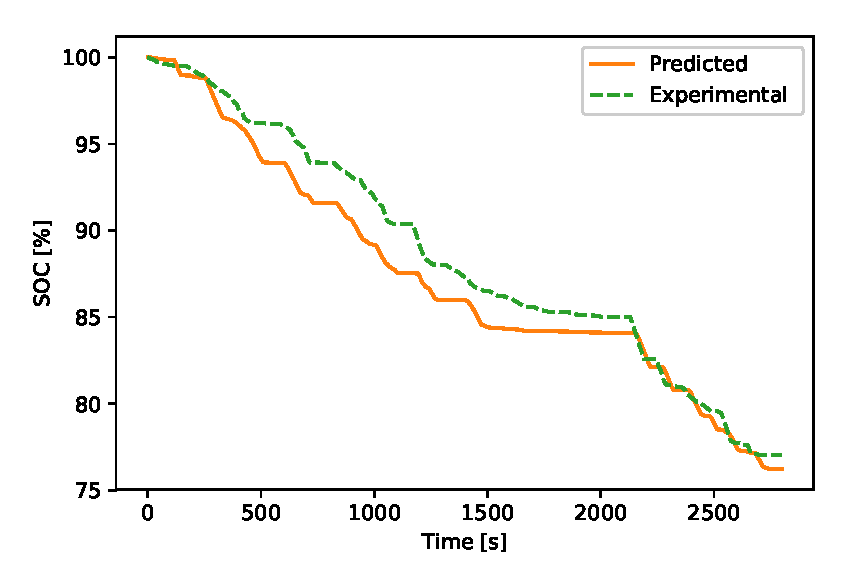
\includegraphics[width=\textwidth]{images/val_soc_2.eps}
    \caption{A comparison of the experimental and predicted SOC depletion over Journey 1}
    \label{fig:val_soc_1}
\end{minipage}%
\begin{minipage}{.5\textwidth}
  \centering
    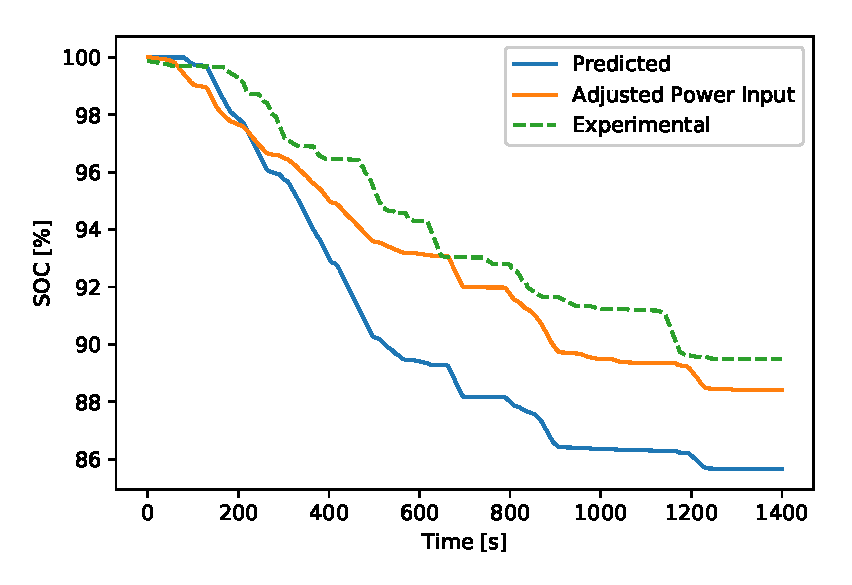
\includegraphics[width=\textwidth]{images/ride2_val_soc.eps}
    \caption{A comparison of the experimental and predicted SOC depletion over Journey 2}
    \label{fig:val_soc_2}
\end{minipage}
\end{figure}


Figure \ref{fig:val_yr4_pas} shows that this year's model (YR5) is much more accurate to the experimental results when compared to last year's model (YR4). Two different model results from year 4 has been presented to illustrate that at either PAS 3 or 4 the model leads to an inaccuracy of more than 5\% (absolute). The largest contributor to the model's improvement is the removal of the assumption that a rider maintains a constant PAS. This can be seen by the year 4 results having a significantly different SOC depletion gradient which will result from an over or underestimate of the PAS setting. Furthermore, improvements are also due to improved estimates for the PAS battery to rider input ratios, the inclusion of internal resistance and OCV relationships with temperature and the more accurate relationship between capacity and temperature.

\begin{figure}[H]
    \centering
    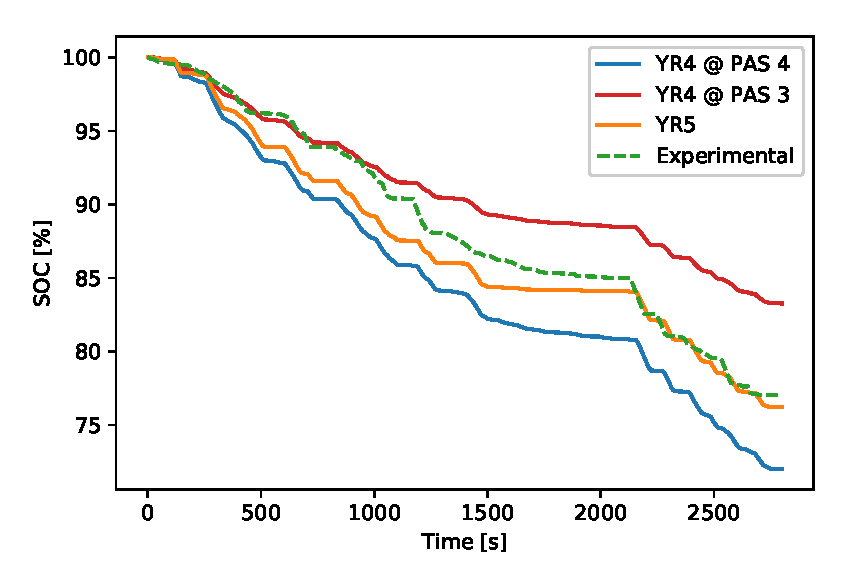
\includegraphics[width=0.5\textwidth]{images/val_yr4_pas.eps}
    \caption{A comparison of the assumptions made in Year 4 and Year 5 models for the PAS selection for Journey 1}
    \label{fig:val_yr4_pas}
\end{figure}

It can be concluded that the model created can accurately predict the SOC depletion of a battery over a journey. Furthermore, it can be seen that the model is much more accurate than the model previously developed.

\subsubsection{Model Evaluation}

This section presents and evaluates the results and findings of the SOC model. The model was run with a common route across all tests to maintain consistency when presenting the results.
\\
\textbf{Discuss rate of SD with SOC}
\\
\\
\textbf{1. Effect of Rider's Preferred Pedal Assist Setting}

Figure \ref{fig:eval_pas} presents the affects of variations in a rider's preferred PAS on level ground. It can be seen that varying the preference from very low (PAS 1) to very high (PAS 5), significantly impacts the final SOC, for the route shown the preference adjusts the final SOC by over 7\% (absolute). Therefore, it is important for a rider to input their preference prior to a journey in order to determine the SOC required and therefore give the rider the most appropriate ebike.

Furthermore, it can be seen that for a 45 minute journey ridden with a preference of PAS 5 on a flat the battery depletes by just over 25\%. Clearly this is very dependant on the route profile but, for the application of public hire ebikes where the average journey length is 19 minutes, the ebike is unlikely to be required to be fully charged \cite{tfl} . Therefore, using this model the DT could be developed to provide the operator with an optimum charging strategy to suit their requirements and the needs of the riders. For example, it the DT may calculate that the ebikes could be left without recharging for a number of rides and only put on to charge when the energy is cheapest (overnight and in the off peak times during the day), this will minimise the operator's operational costs.

\begin{figure}[H]
    \centering
    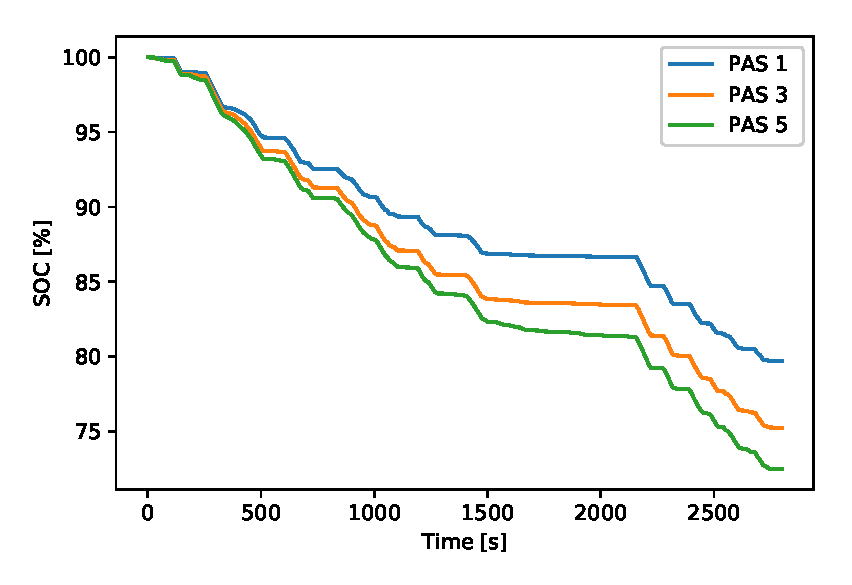
\includegraphics[width=0.5\textwidth]{images/eval_pas.eps}
    \caption{A comparison of the effect of a rider's chosen pedal assist setting on the SOC depletion}
    \label{fig:eval_pas}
\end{figure}



\textbf{2. Effect of Ambient Temperature}

Figure \ref{fig:eval_op_temp} illustrates the effect of cycling (operating) temperature on the performance of the battery and the impact on required SOC for a given journey. It can be seen that at lower temperatures, it is necessary to monitor the ambient temperature as for this route the SOC required varies by 5\% (absolute) between -5\degree C to 15 \degree C. These results include the temperature affect on capacity, OCV and internal resistance. Table \ref{tab:temp_soc_jazz} presents the variations in final SOC for the given journey when the effect of temperature is captured for the different battery features. The table shows that the temperature dependency of the battery's capacity has the greatest impact on the final SOC. Whereas including the effects of temperature on OCV and internal resistance has a smaller impact on required SOC. From this it can be concluded that for an application whereby the SOC prediction does not need to be accurate to large significant figures, a model just capturing the effects of temperature on capacity would be satisfactory. Furthermore, as the temperature effects on internal resistance and OCV when considering the overall SOC calculation are small the empirical formulas used to define the relationships are satisfactory. This, therefore, avoids the extensive temperature testing a battery would require to deduce the exact relationships with capacity, OCV and internal resistance. Table \ref{tab:temp_soc_jazz} also compares the results from the previous model, which only included the temperature's effect on capacity and assumed that there was no impact about 10 \degree C. It can be seen that the assumptions made previously were inaccurate against the empirical relationships used in the developed model, especially at lower temperatures.


\begin{figure}[H]
    \centering
    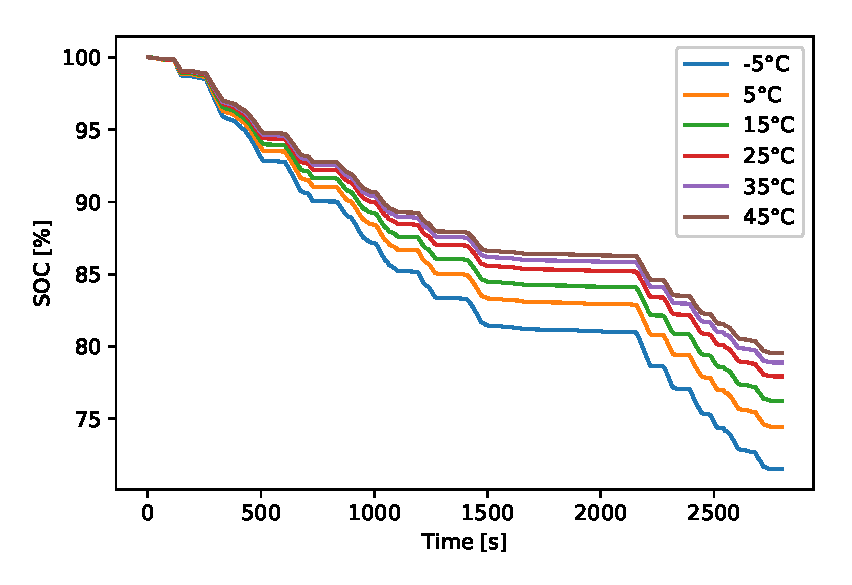
\includegraphics[width=0.5\textwidth]{images/eval_op_temp.eps}
    \caption{A comparison of the effect of the operating temperature on the SOC depletion}
    \label{fig:eval_op_temp}
\end{figure}

\begin{table}[H]
\centering
\caption{The effect of temperature on different battery features and the final SOC of a given journey}
\label{tab:temp_soc_jazz}
\begin{tabular}{|P{0.15\textwidth}|P{0.14\textwidth}|P{0.14\textwidth}|P{0.14\textwidth}|P{0.14\textwidth}|P{0.14\textwidth}|}
\hline
\multirow{2}{*}{Temperature (\degree C)} & \multicolumn{4}{c|}{Temperature Relationship Included to Predict Final SOC} & \multirow{2}{*}{Previous Model} \\ \cline{2-5}
& All & Only Capacity & Only OCV & Only Internal Resistance & \\ \hline
-5          &  71.51\%   &  72.10\%  &  77.86\%  &  77.49\% &  62.72\% \\ \hline
20          &  77.14\%   &  77.33\%  &  77.78\%  &  77.80\% & 78.77\% \\ \hline
45          &  79.57\%   &  79.68\%  &  77.74\%  &  77.88\%  & 78.77\% \\ \hline
\end{tabular}
\end{table}



\textbf{3. Effect of State of Health}

Figure \ref{fig:eval_soc_soh} presents the effects of the SOH of the battery on the SOC depletion over a given journey. The figure shows that if a battery's SOH degrades by 20\% the SOC requirement increases by over 5\%. Furthermore, it also shows that as the SOH degrades, the rate at which the SOC requirement increases increases. Table \ref{tab:soh_IR_cap} presents the impact of modelling the SOH's relationship with capacity and internal resistance on the final SOC of the given route. It can be seen that SOC results are predominately impacted by the effect of SOH on capacity, whereas the impacts on internal resistance are relatively small. It can be concluded that to produce an accurate SOC model the affect of SOH must be captured in order to maintain the model's accuracy as the battery ages and that unless a model needs to be highly accurate, the effects of SOH on internal resistance can be ignored.


\begin{figure}[H]
    \centering
    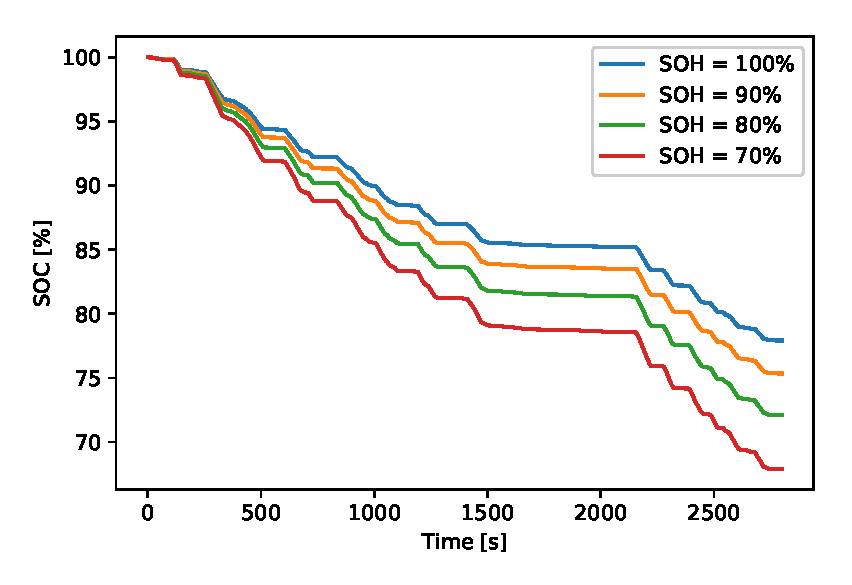
\includegraphics[width=0.5\textwidth]{images/eval_soc_soh.eps}
    \caption{A comparison of the effect of SOH on the SOC depletion}
    \label{fig:eval_soc_soh}
\end{figure}

\begin{table}[H]
\centering
\caption{The effect of SOH on different battery features and the final SOC of a given journey}
\label{tab:soh_IR_cap}
\begin{tabular}{|P{0.10\textwidth}|P{0.14\textwidth}|P{0.14\textwidth}|P{0.14\textwidth}|}
\hline
\multirow{2}{*}{SOH (\%)} & \multicolumn{3}{c|}{SOH Relationship Included to Predict Final SOC}\\ \cline{2-4}
& All & Only Capacity & Only Internal Resistance \\ \hline
100 &  77.92\%   &  77.92\%  &  77.92\%   \\ \hline
90 &  75.12\%   &  75.35\%  &  77.74\%   \\ \hline
80    &  71.60\%   &  72.01\%  &  77.55\%  \\ \hline
70   &  70.00\%  &  67.85\%  &  77.34\%   \\ \hline
\end{tabular}
\end{table}

\textbf{what happens at 70\%????}

\textbf{5. Effect of Self Discharge}

\subsubsection{Sensitivity Analysis}

This section presents the results of the sensitivity analysis conducted. Analysis concentrated on evaluating the impact of the assumptions made (in Table \ref{tab:soc_assump}) and those that were estimated to produce the greatest inaccuracies in the model.
\\
\\
\textbf{1. Motor Efficiency}

It was assumed that the motor's efficiency remained constant at 60\% throughout the journey. However, as has been discussed earlier, in practice the motor's efficiency can vary greatly, depending on the torque on the motor. Figure \ref{fig:SA_motor_eff} presents the sensitivity of the model's results to the assumed motor efficiency. The model was run at efficiencies of 50\%, 60\%, 70\% and 80\%. It can be seen that by varying the motor's efficiency the final SOC can vary by up to 3\% (absolute). For this route, it can be seen that a motor efficiency of 70\% gives a more accurate final SOC. This indicates that an assumption of 60\% efficiency is an adequate assumption for this application but variations in efficiency should be captured if a highly accurate result is desired.

\begin{figure}[H]
    \centering
    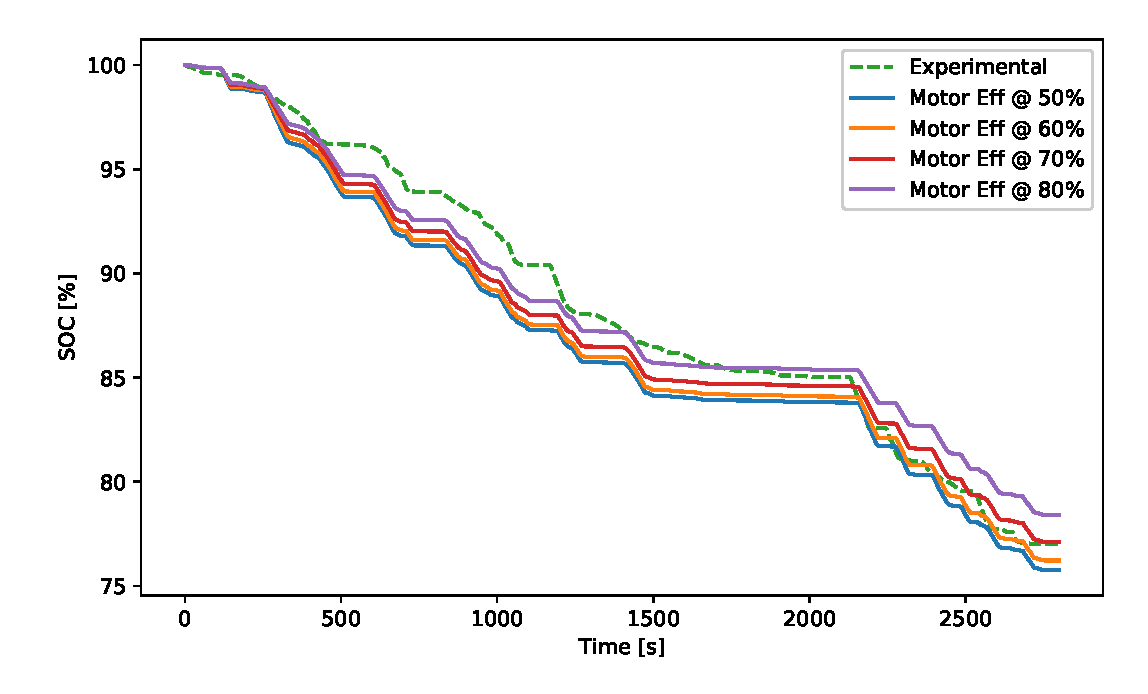
\includegraphics[width=0.6\textwidth]{images/SA_motor_eff.eps}
    \caption{A comparison of the sensitivity of motor efficiency on the SOC depletion}
    \label{fig:SA_motor_eff}
\end{figure}

\textbf{2. Rider Input Power}

The model assumed that the rider input a constant power across the journey (up to the point at which the battery power reached its upper limit and the rider then input more power to maintain a constant velocity). However, in practice a rider's input power (and velocity) is expected to vary along a route. To evaluate the model's sensitivity to this assumption the model was tested with rider input powers at 20\% higher and lower than the expected norm (which was based on rider weight and a constant velocity of 7m/s in no wind). A variation of 20\% was deemed a suitable variation as on average a rider would wish to maintain a constant input power. Figure \ref{fig:SA_rider_p} presents the results of the sensitivity test, showing that the final SOC varied by 2\% (absolute). It can be seen that a rider power of 20\% greater than assumed gives a closer correlation to the final SOC. However, the difference is small and therefore indicating that assuming a constant rider power input is sufficiently accurate.

\begin{figure}[H]
    \centering
    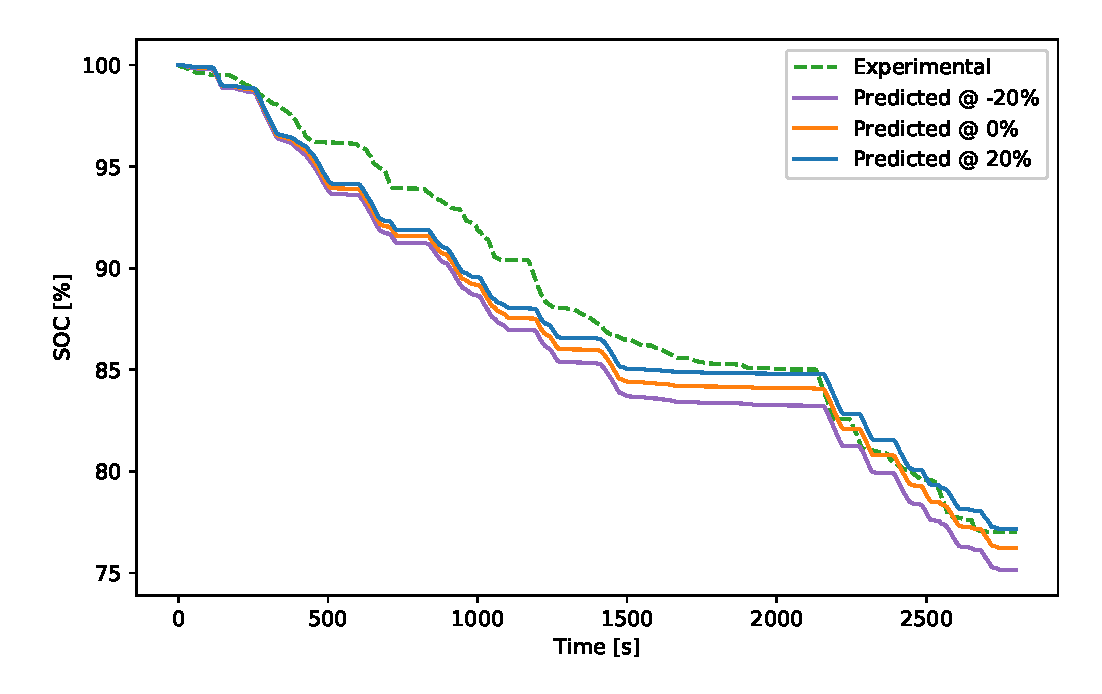
\includegraphics[width=0.6\textwidth]{images/SA_rider_p.eps}
    \caption{A comparison of the sensitivity of rider input power on the SOC depletion}
    \label{fig:SA_rider_p}
\end{figure}



\textbf{Could also do: Capacity-Temperature Relationship Sensitivity}


Probably conclude for the SOC model that results are quite sensitive and so need to do more through battery testing.

\subsubsection{Conclusions and Future Development}

The results have shown that a highly accurate SOC model has been designed, which captures the variance in rider styles, the impact of the environment on performance and the impact of battery ageing. This model can be used alongside the dynamics model to accurately predict the charge requirements of a journey, which then allows the operator of a fleet of public hire ebikes to release the most appropriate bike to the rider.

\textbf{I would say here that the model can be used by manufacturer to optimise capacity but this is only discussed in George's section- advice?}

It has been identified that in order to accurately model SOC the following battery characteristics need to be captured: variations in OCV, internal resistance, capacity, SOH and self discharge.
It has been shown that the ambient temperature and SOH have the most significant affect on the available capacity, whereas, the impact on the OCV, internal resistance and self discharge is small and do not considerably change the battery's performance. Therefore, the empirical formulas used to define the relationships with OCV, internal resistance and self discharge are satisfactory for model definition and extensive thermal and ageing testing is not necessary. However, capacity and therefore SOC varies significantly with temperature and so it is advised that a manufacturer conducts battery testing to calculate the exact relationship for a given battery instead of using the empirical formula relationship used in this model.

The model produced is accurate although it has been shown that its results are sensitive to a number of assumptions. Therefore, in the future, the model should be updated to capture the variance of motor efficiency with torque instead of assuming it to be constant at 60\%. Furthermore, it was identified that different riders may have varying riding and power input styles therefore if this variance is deemed to be large enough then a machine learning aspect could be incorporated into the model to predict for a given rider how their PAS and power input will vary for a given journey.

Further possibilities of the model's capabilities include providing the optimum PAS to the rider across a route to not only aid the rider's journey but also minimise any degradation on the battery. Also as discussed earlier, the model could be used by the operator in order to optimise charging strategies to both extend the life of the battery and minimise the operational costs of the fleet by charging the bike's when energy is cheapest.

\newpage

\section{Predicting Battery Degradation}
\label{section:SOH}

%Intro into why we are looking at SoH

SoC looks at the characteristics of the battery within a single cycle. However, it is also important to consider how the characteristics of a battery change with time and discharge cycles, as this has an effect on both the SoC and the lifespan of the battery. This characteristic is known as the battery's state of health (SoH). Specifically, SoH describes the percentage of full charge capacity (FCC) that the current battery is capable of compared to its initial FCC (\ref{eq:SOH}). FCC is the maximum amount of charge a battery can hold.

\begin{equation}\label{eq:SOH}
    SoH = \frac{FCC}{FCC_{initial}}\times100
\end{equation}

SoH can be used to measure the lifespan of the battery. This is performed by determining  the time span or the number of cycles before the battery reaches an SoH of $<80\%$, after which the battery is said to be redundant \cite{ISO}. For Li-ion batteries, as used on the ebike, this would translate to a lifespan of typically 500 to 1200 cycles \cite{web:batt_life}. However, the unique usage pattern on fleet ebikes could have a substantial effect on the lifespan and therefore the SoH needs to be investigated.

%how batteries degrade
%The FCC of a Li-ion battery decreases due to two mechanisms, side reactions and mechanical stress \cite{report:ageingmechs}. Side reactions are when the electrolyte irreversibly bonds to the anode, leading to the FCC and coulombic efficiency decreasing \cite{report:sidereactions}\cite{report:ageingmechs} and is enhanced by high temperatures, large c-rates and high SoC. Whereas mechanical stress results in the node materials developing micro-cracks and is exacerbated by increasing the depth of discharge and high c-rates, impacting the FCC \cite{report:ageingmechs}

The following sections will identify the causes and effects of SoH and address the merits of different modelling techniques. Following this, a model will be defined and created that can be used to predict battery degradation for an ebike, allowing for an optimal battery capacity to be suggested.

\subsection{Factors Affecting SoH} 
The factors affecting battery degradation can be split into two categories, calendar life and cycle life. Calendar life factors affect the batteries capacity to store charge due to the passing of time, whether or no the battery is cycled. These factors include storage temperature and SoC during storage \cite{report:batterypred}. Cycle life factors occur because of the charging and discharging of the battery and are dependent on the number of cycles, temperature, rate of charge/discharge, average SoC and depth of discharge \cite{report:Lam}. Compared to cyclic degradation, calendar degradation is small, therefore in the SoH model only cyclic degradation will be considered. 

%%Literature on the effects each of the factors have on battery SoH will be reviewed and will allow for a model to be produced that predicts how different scenarios will affect the life of a battery. The outcome of the model will be a suggestion of a optimal charging strategy and battery specifications for the specific use in a ebike fleet.

%%maybe use instantaneous discharge voltage determine how SoH varies as it fits? however number of cycles could still be used, depends on what is easier as the correlation between 100\% and 80\% is still good for cycle number [Regression Models Using Fully Discharged Voltage and Internal Resistance for State of Health Estimation of Lithium-Ion Batteries] [An Online SOC and SoH Estimation Model for Lithium-Ion Batteries]

\subsubsection{Number of Cycles}
During each cycle, degradation of the battery's SoH occurs. This is due to the cyclic mechanical stress and passivation on top of the other cyclic degradation factors. Mechanical stress occurs due to the insertion and ejection of lithium ions resulting in a volume change of the electrodes \cite{web:batt_life}. This physical change in volume, results in micro-cracks forming, reducing the FCC of the battery \cite{report:ageingmechs}. Whereas passivation occurs due to the irreversible deposition of a resistive layer known as the solid electrolyte interface which impedes chemical reactions as well as increasing internal resistance \cite{report:ageingmechs}.

%try a find a nice graph showing the decay of SoH with the number of cycles. or an equation that describes the curve

\subsubsection{Operating Temperature}

The operating temperature affects both the SoC and the SoH. At higher temperatures the available capacity for a given journey is greater however operating at higher temperatures degrades the battery faster \cite{web:batt_life}\cite{report:Arrhenius}. At higher temperatures, faster chemical reactions within the battery can occur and are what leads to the initially larger capacity. However, the increased number of chemical reactions also speeds up the rate at which micro-cracking and passivation occurs. 
To describe the relationship between temperature, chemical reactions and battery degradation the Arrhenius equation can be used:
\begin{equation}
\label{eq:Arr}
    y=Ae^{\big(\frac{E_a}{RT}\big)}
\end{equation}
where $y$ is the rate of chemical reactions, $A$ is the frequency factor relating the number of collisions between molecules, $E_a$ is the activation energy, $R$ is the gas constant and $T$ is temperature in Kelvin. Operational temperature takes into account the temperature of the environment as well as the battery due to ohmic heating. Operational temperature is therefore related to the rate of charge/discharge.

\subsubsection{Rate of Discharge}\label{RoD}

The rate at which current is drawn or applied to the battery is known as the c-rate and is scaled to the capacity of the battery. A current of 1C would, therefore, be defined as the current to charge or discharge the battery in one hour. Likewise, a current of 2C would charge/discharge the battery in half an hour. 

Charging/discharging a battery at a rate greater than 1C results in the SoH decreasing at a faster rate than that of 1C. This is due to several irreversible damage mechanisms including lithium plating and micro-cracks forming in the nodes \cite{web:batt_life}. Though the charging/discharging  effect is well know, there has been little research into detailing the relationship between c-rate and SoH, with models only describing the relationship empirically. This, therefore, requires the battery type to be physically tested to identify how the c-rate will affect the SoH, taking a significant length of time. Being able to model the effects of c-rate without the need to run tests would, therefore, present a substantial benefit. Unfortunately, however, this is outside the scope of this report.

In the case of an ebike, the c-rate would vary based on the pedal assist which would likely vary over the course of the journey. However, for the model, it will be assumed that an average of the c-rate over the entire journey will produce an accurate enough result.

\subsubsection{Depth of Discharge} 
Depth of discharge (DoD) is generally defined as the percentage drop in SoC from the FCC during a cycle \cite{report:doddef}. However, this definition assumes that the battery is always discharged from full. For example, a battery discharged from an SoC of $100\%$ to $40\%$ and a battery discharged from $60\%$ to $40\%$ would both be described as having a DoD of $40\%$. Instead, $\Delta$DoD can be used to help capture the charge in DoD. However, ideally, both DoD and $\Delta$DoD would be used to describe battery discharge. This is because cycling in the upper portion of the battery's capacity is less damaging than cycling in the lower portion (need to find a ref for this). The exact effect of cycling in different portions of the battery is not well defined, therefore for the rest of the report it will be assumed that the battery will always be discharged from full. The relationship between DoD and SoH is however well described and follows the relationship described by equation \ref{eq:DoD} \cite{report:NASADoD}, where $L$ is the number of cycles, $B$ is a constant and $D$ is the depth of discharge as a fracture of the rated capacity. An example of how this effects SoH is shown by Figure \ref{fig:dod}. Through the graph is for a lead acid battery the relationship is the same for a lithium-ion battery.

\begin{equation}\label{eq:DoD}
%L=L_\phi e^{\alpha(1-D)}
L=B\frac{1-D}{D} 
\end{equation}

\begin{figure}[H]
    \centering
    \includegraphics[width=0.6\linewidth]{images/dod.png}
    \caption{Relationship between DoD and cycle life for a lead acid battery \cite{web:batt_life}.}
    \label{fig:dod}
\end{figure}

\subsubsection{Average SoC} \label{sec:aveSoC}
The SoC has a noticeable effect on the SoH of a battery. The higher the SoC, the more energy is being stored, accelerating the degradation process. This is because more reactions take place, increasing the development of the solid electrolyte interphase layer \cite{book:aveSoC}. During cycling, the effects of SoC are minimal as it is continuously changing. However, cycling in the upper portion of the battery would result in faster degradation than cycling in the lower portion, due to the average SoC being higher. The SoC the battery is stored at has a much greater effect due to the increased length of time the SoC is maintained. The effects SoC has on SoH is described by the Tafel equation, Equation \ref{eq:tafel} \cite{pres:tafel}:

\begin{equation} \label{eq:tafel}
    a_1=a_{1_{ref}}e^{\big(\frac{\alpha F}{RT}V\big)}
\end{equation}

Taking into account the effects of both DoD and SoC on SoH, the battery would want to be discharged to different depths depending on its usage pattern. If the battery is in regular use with only short periods of downtime, it would be preferable to operate the battery in the upper portion of its capacity, minimising the negative effects of large discharge cycles. Whereas if the battery is likely to experience long periods of downtime after use, the negative effects of the increased depth of discharge to reduce the SoC the battery is stored at would be migrated, slowing the degradation of the battery.

\subsection{Methods of Modelling State of Health}
To ensure the most suitable modelling technique is used for the SoH model, a review of techniques has been carried out in the following sections.

\subsubsection{Cycle Number}

One of the simplest methods of modelling and predicting the SoH of a battery is using the cycle number. The relationship can be defined by Equation \ref{eqn:SoH_cycles}.

\begin{equation}
    SoH_{N} = \gamma_{1}N^{2}+\gamma_{2} N + \gamma_{3}
\label{eqn:SoH_cycles}
\end{equation}

Where \textit{N} is the number of cycles and $\gamma$\textsubscript{i} are model coefficients \cite{report:Regression_SoH}. 
However, this method of modelling does not take into account the impact of use and environment on the SoH. Furthermore, it is not suitable for an ebike application as a fleet of ebikes is unlikely to be fully discharged and charged during and after a journey and therefore are not full cycles.


\subsubsection{Electrochemical}
Electrochemical modelling aims to model the  processes that lead to the degradation of the SoH and then relating that to the SoH rather than modelling SoH directly. This has the benefit of producing parameters with physical meaning, allowing for a better understanding of how the battery is degrading and affected by the adverse conditions.

Electrochemical models vary in the computational requirements and detail and can range from modelling every molecule in the case of Molecular Dynamics, to Single Particle Modelling which models a single electrode particle that representing the average \cite{report:electro}. Obviously, these types of models are highly computationally expensive and currently limited validation. Furthermore, detailed knowledge of the battery's composition is required, which is something that is not possible in the case for the ebike battery being studied in this report. Though due to computational and practical limitations this method is not currently feasible, electrochemical modelling will likely soon become a realistic model choice due to better validation and reduced computational demand.

\subsubsection{Internal Resistance}

Through monitoring and predicting the internal resistance of the battery the SoH can be calculated and predicted because as the battery ages the internal resistance increases. It has been found that the relationship between SoH and internal resistance is as follows:

\begin{equation}
    SoH = \frac{R-R_{aged}}{R_{new}-R_{aged}}
\label{eqn:SoH_IR}
\end{equation}

Where \textit{R} is the present internal resistance, \textit{R\textsubscript{new}} is the internal resistance at the beginning of the battery's life and \textit{R\textsubscript{aged}} is the internal resistance at the end of the battery's life. \textit{R\textsubscript{new}} and \textit{R\textsubscript{aged}} are known values and \textit{R} can either be measured or predicted \cite{report:IR_SoH}. To predict \textit{R} the following equation can be used:

\begin{equation}
    R(T,I) = ae^{l} + bI^{m} + c
\end{equation}

Where \textit{a}, \textit{b} and \textit{c} are coefficients of the exponential function, \textit{l} and \textit{m} are the exponents of the exponential function \cite{report:IR_SoH}. Although this method accounts for the impact of temperature (T) and rate of discharge (I) on internal resistance, it doesn't account for the number of cycles, average SOC and depth of discharge.

Alternatively, the internal resistance of the battery could be monitored throughout the ebike's operation. The SoH could then be calculated and monitored using Equation \ref{eqn:SoH_IR}. However, this does not create a predictive model. Furthermore, measuring the internal resistance remotely is costly as it would require both a voltage and current sensor.

\subsubsection{Stress Factor}

The stress factor method models the fade in capacity rather that SoH itself. This therefore still allows the battery's future SoH to be predicted, without needing to know how many cycles the battery has already performed. All that is needed is the rated FCC, the current FCC and the stress factor parameters that are predetermined by the battery. This method also has the additional benefit of taking into account different DoDs, utilising the energy discharged per step, rather than just cycle number. The total drop in SoH can be calculated by equation \ref{eq:SoH}. Equation \ref{eq:SoHstep} shows the method of calculating the drop in SoH per step. By having each increment as a step rather than a discharge cycle allows for each cycle to be broken down into steps that have the same stress factors, thus producing a much more accurate prediction.

The model takes into consideration the effect temperature ($\sigma_T$), discharge rate ($\sigma_C$) and SoC ($\sigma_SoC$) have on the rate of SoH degradation. These conditions are then scaled by the stress factor parameter $k$, to relate them to the drop in SoH per cycle. $k$ is used to scale the effects that adverse conditions have on the battery's SoH, while $k_1$ is used to scale the drop in SoH under reference conditions. Under reference conditions, all stress factors are 1. Additionally, the effect DoD has on the number of cycles to failure is also taken into consideration thanks to $\Delta Ah$, which is the amount of energy discharged per step. $\Delta Ah$ is used to scale the impact of the degradation, therefore if less energy is dissipated per cycle, less degradation occurs, therefore accounting for the reduced DoD. Below, more detailed is provided on how the different stress factors are calculated.

\begin{equation}
\label{eq:SoH}
    \xi=\sum_{i}^{E}\Delta\xi_i
\end{equation}
\begin{equation}
\label{eq:SoHstep}
    \Delta\xi_i=\frac{1}{2}k_{\sigma_i}\Delta Ah_i^2+\Delta Ah_i\sqrt{k_1^2+2k_{\sigma_i}\xi_{i-1}}
\end{equation}
\begin{equation}
    k_{\sigma_i}=k\sigma_T\sigma_C\sigma_{SoC}
\end{equation}
%\sigma_I=$ c-rate stress factor\\
%$k_2 =$ a scaling constant for reference conditions\\
%$\sigma_T , \sigma_I =$ 1 at reference conditions

\subsubsection*{Temperature}
As discussed previously, temperature has a large impact on the rate that SoH decreases with the relationship between temperature and SoH being described well by the Arrhenius Equation \ref{eq:Arr}. This equation is modified into Equation \ref{eq:temp} to define the temperature stress factor which produces a value of 1 at the reference temperature.

\begin{equation}
\label{eq:temp}
    \sigma_T(T,\xi)=\sigma_{Tref}e^{\bigg(-\frac{E_a(\xi)}{R}\big(\frac{1}{T}-\frac{1}{T_{ref}}\big)\bigg)}
\end{equation}

$E_a$ is dependent on SoC during storage and the time stored, however, no clear relationship has been found. For simplicity, it can be assumed to be constant. 

\subsubsection*{C-Rate}
As mention in Section \ref{RoD}, degradation from c-rate is a complex relationship and currently can only be found experimentally. The relationship can then be described using a second order polynomial which can then be used to describe the c-rate stress factor, Equation \ref{eq:cstress}. The c-rate stress factor is dependent on both the c-rate and the battery's current SoH and must, therefore, be calculated for each SoH.

\begin{equation}
\label{eq:cstress}
    \sigma_I=k_3(\xi)+k_4(\xi)I+k_5(\xi)I^2
\end{equation}


\subsubsection*{SoC}
As described in Section \ref{sec:aveSoC}, the degradation effects of SoC can be modelled using the Tafel equation \cite{book:aveSoC}. This equation can then be manipulated in the Equation \ref{eq:sigma_SoC}.

\begin{equation}
\label{eq:sigma_SoC}
    \sigma_{SoC}=\sigma_{SoC_0}e^{\big(\frac{\alpha F}{RT}V\big)}
\end{equation}


\subsection{Evaluation of Modelling Methods}

%\begin{table}[H]
%    \centering
%    \caption{Factors Impacting and Impacted by SoH}
%    \begin{tabular}{|P{0.25\textwidth}|P{0.25\textwidth}|P{0.25\textwidth}|}
%    \hline
%       \textbf{Factors} & \textbf{Factors Imapcting SoH}  & \textbf{Factors Impacted by SoH}
%        \\
%        \hline 
%        Depth of Discharge & \checkmark & 
%        \\
%        \hline 
%       Rate of Discharge & \checkmark & 
%             \\
%        \hline 
%        Operating Temperature & \checkmark & 
%             \\
%        \hline 
%        Average SOC & \checkmark &
%            \\
%        \hline 
%        Internal Resistance & & \checkmark
%             \\
%        \hline 
%       OCV-SOC Curve &  & \checkmark
%        \\
%         \hline 
%       Self Discharge &  & \checkmark
%        \\
%\hline
%    \end{tabular}
%    \label{tab:SoH_Lit_Review}
%\end{table}

To allow for easy comparison between methods Table \ref{tab:SoH_summary} was generated to 
summarises the functionality and suitability of each modelling technique. From this, it was concluded that the stress factor method should be used to model SoH. This decision was based on the range of adverse conditions that it can model, as well as the modular nature of the stress factors, allowing for easier model development.

\begin{table}[H]
\caption{Summary of Methods to Model SoH}
\centering
\begin{tabular}{|l|c|c|c|c|}
\hline
 & \textbf{Cycle Number} & \textbf{Chemical} & \textbf{Stress Factor} & \textbf{Internal Resistance} \\ \hline
Impact of number of cycles  & Y & Y &Y  & N  \\ \hline
Impact of temperature  & N & Y & Y & Y     \\\hline
Impact of rate of discharge & N & Y & Y & Y  \\\hline
Impact of depth of discharge  & N & Y & Y & N  \\\hline
Impact of average SOC  & N & Y & Y & N       \\\hline
Ease of implementation  & High  & Very Low  & Moderate &   Moderate  \\\hline
Applicability to ebike application & Low & Moderate & High &     Moderate 
\\\hline
\end{tabular}
\label{tab:SoH_summary}
\end{table}

\subsection{State of Health Model Definition}
%An assumption of this model was that the battery was new and was at 100\% SoH at the beginning of this year (completely not true)

%Model purpose/objective?
The purpose of the SoH model is to provide the operator with the ability to monitor and predict the capacity fade of a battery until its end of life at $80\%$ SoH under varying conditions and usage patterns. This provides value to the operator as it allows them to identify when batteries need replacing, With the correct implementation it could also allow for the operator of a fleet to alter usage patterns to better optimise the performance of the fleet. Additionally, being able to predict battery degradation would allow for the designers of the ebike to make a better informed decision on what battery they should use.

Figure \ref{fig:SoHprocess} displays the modelling process, defining the required inputs and resulting outputs. Initially, the type of battery to be implemented within the DT is tested under specific discharge rates and temperatures. This allows for the rate of damage for a given condition to be calculated. For c-rate, this must be calculated for each SoH as the damaged caused by c-rate is also dependent on the battery's current SoH. Using equations \ref{eq:cstress} and \ref{eq:temp}, the stress factors can be found. The stress factor parameters $k_1$ and $k$ are then varied in equation \ref{eq:SoHstep} to fit the modelled degradation profile with the experimental profile to find $k_1$ and $k$ for the specific battery. Then, to modelled the battery on the ebike, the SoC model is used to record the current and historic DoD and discharge rates, which is combined with the ambient temperature to find the temperature of the battery. These values are then used in the SoH to find the current SoH. The same process can then be carried out using the predictive dynamics model to predict the number of cycles until the battery needs replacing.

\begin{figure}[H]
    \centering
    \includegraphics[width=1\linewidth]{images/SoH_model_diagram.png}
    \caption{SoH Modelling Process.}
    \label{fig:SoHprocess}
\end{figure}

\subsubsection{Assumptions}
Due to the limited time frame and scope of this report, several simplifications and assumptions have been made when implementing the stress factor method. The assumptions made are listed in Table \ref{table:SoHass}.

\begin{table}[H]
\caption{SoH model assumptions}
\label{table:SoHass}
\begin{tabular}{|P{0.2\textwidth}|P{0.3\textwidth}|P{0.3\textwidth}|P{0.1\textwidth}|}
\hline
\textbf{Assumption} & \textbf{Discussion/Limitation} & \textbf{Justification} & \textbf{Impact}
\\
\hline
Stress factors are constant within individual battery cycles & Stress on the battery will vary during a ride due to changing demands placed on the motor and battery. The assumption was made to limit the complexity of the model  & Though it is highly dependent on ebike usage, stress factors would likely remain mostly constant with only short peaks and troughs across the entirety of a users journey. An average of the stress factors over the course each ride has therefore been deemed acceptable & Low
\\
\hline
Stress due to average SoC is negligible  & Neglecting stress due to SoC ignores some of the degradation that the battery experiences and would therefore produce an optimistic value of SoH & SoC has minimal affect on SoH for Li-ion batteries that are regularly cycled. Therefore, degradation lost due to SoC is negligible & Low
\\
\hline
The battery is always discharged from full & This impacts the stress due to DoD as the degradation caused by the amount of capacity discharge is dependent on which portion of the battery was discharged & There are conflicting relationships between battery degradation and which portion the battery is cycled in \cite{report:cho}\cite{report:peterson} & Medium
\\
\hline
The battery experiences stress due to temperature that is representative of the data presented by \cite{web:batt_temp} & Battery temperature severely affects the life of a battery due to speeding up or slowing down the chemical damage mechanisms that result it the reduction in capacity & There is no data available for how temperature affect the battery used on the ebike. Therefore, the data used, is used to demonstrate the effect of temperature, rather than provide an accurate model of it & High
\\
\hline
The battery used on the ebike has the same damage characteristics as the one found in the literature \cite{report:cho} & Each specification of battery will have different stress factor parameters and therefore respond to stress differently, producing an individual degradation profile & There is a several lack of suitable data on the degradation of batteries. The data found in Choi et el best represented the ebike battery and suited the needs of the model. Without fully degrading the battery is specific degradation profile and stress factor parameter can not be found & High
\\
\hline
Battery degradation due to calendar ageing is negligible & With fleet ebikes being a product that spends its entirety of its life outside, it experiences a significant range of conditions that effect the rate of calendar ageing, predominately temperature & Loss of SoH due to calender ageing is negligible compared to that caused by cyclic ageing & Low
\\
\hline
\end{tabular}
\end{table}


%\subsubsection{State of Health Modelling Process}

%talk about process. process the same between batteries but coefficients differ. therefore process much be performed for each different battery type.

%For every specification of battery  that wants to be modelled, experimental testing must be carried out as the stress factor parameters ($k,k_2,k_3,k_4,k_5$) will differ for each battery. Additionally, they themselves can not be modelled or predicted as they represent purely empirical values. The required data and process to calculate these values and then model the SoH of a battery is shown in Figure \ref{fig:SoHprocess}.


%k1 find by $\xi=k_1n+k_2\sqrt{n}+\xi_0$ to SoH-cycle curve. it stays the same even if conditions change.\\
%$k_3, k_4, k_5$ can be found as $\sigma_I=1$ at 1C. a 3d plot of the SoH, cycle, c-rate graph needs to be made, amd the curve joining points at equal SoH detailed as a polynomial. the k-values can then be found as $\sigma_I=1$ when discharge is 1C
%using $\sigma_I=k3(\xi)+k_4(\xi)I+k_5(\xi)I^2$\\
%for $\sigma_T$ $E_a$ can be found using curve fitting 

\subsection{State of Health Model Results}

As has been discussed, for a reliable and accurate SoH model, a significant amount of data needs to be collected for the specific battery. In the case of the battery used on the ebike evaluated in this report, it was not feasible within the time-frame to perform the required experiments. Additionally, severally batteries would be needed to test the batteries at different conditions, something that the authors did not have access to. Therefore, the data required to formulate the stress constant had to be gathered from the literature \cite{report:cho}\cite{web:batt_life}. %After concluding an extensive review of literature, few suitable data sources were identified. Therefore, rate of degradation was collected to from two sources to test the functionally of the model (cite). 


\subsubsection{Identification of Stress Factor Parameters}
\begin{figure}[h]
\centering
\begin{minipage}{.5\textwidth}
  \centering
    \includegraphics[width=0.95\linewidth]{images/ks.png}
    \caption{Stress factor parameter optimisation.}
    \label{fig:ks}
\end{minipage}%
\begin{minipage}{.5\textwidth}
  \centering
    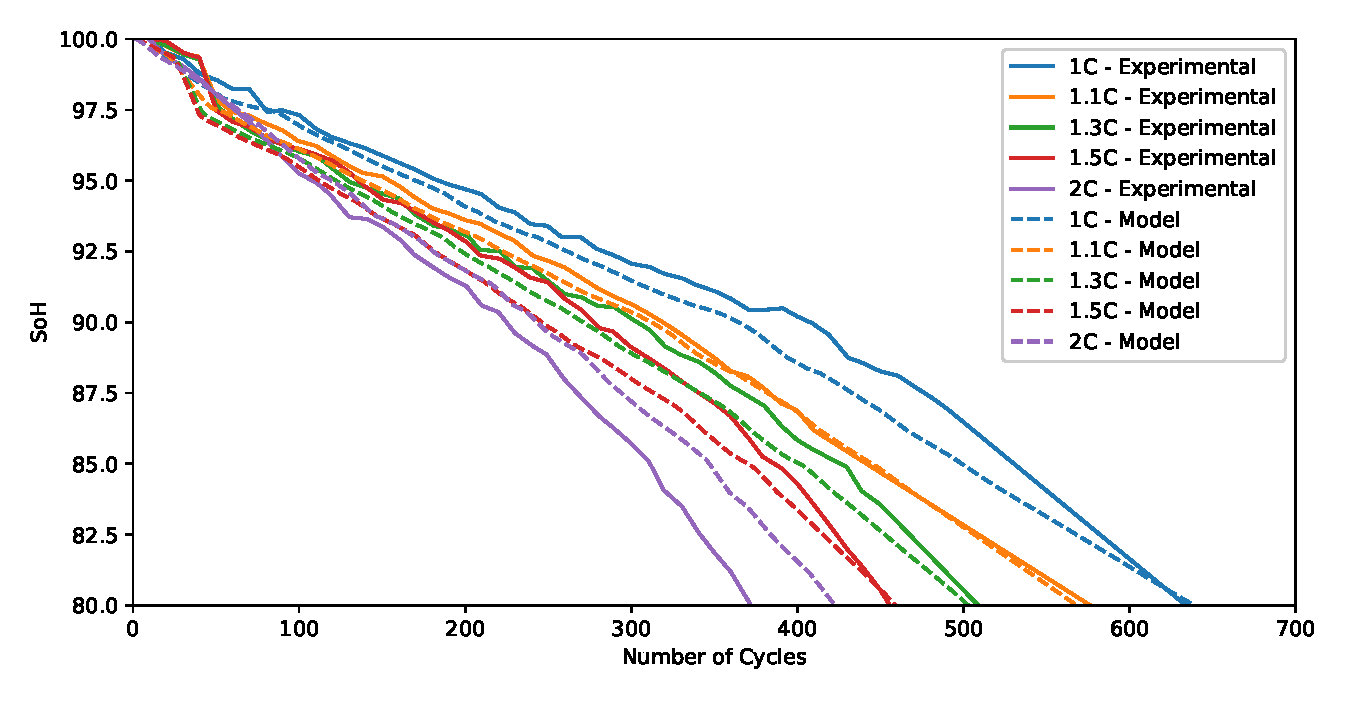
\includegraphics[width=0.95\linewidth]{images/F2_SoH_expVmodel.eps}
    \caption{Comparison of experimental and modelled battery degradation.}
    \label{fig:SoH}
\end{minipage}
\end{figure}

%convergence graph
%state process
%state values
%state improvement to process
The first step in the process of modelling the SoH of the battery was to identify the stress factor parameters $k$ and $k1$. This was achieved by beginning with an initial guess and then varying the  two values and until the  difference between the experimental and modelled degradation profile was at a minimum. The experimental and modelled degradation profiles are shown in Figure \ref{fig:SoH}. Figure \ref{fig:ks} illustrates the process of minimising the difference, identifying $k=0.0133$ and $k1=0.0157$ as the stress factor parameters for the battery found within the literature \cite{report:cho}.These values would be different for the battery used on the ebike, however, it wasn't possible to model it as it was not possible to degrade the battery's SoH in the time available. It can be seen that there is a relatively strong agreement between the modelled data and the experimental data for the number of cycles until failure. With the largest deviation of $13.4\%$ occurring at a c-rate of 2. Agreement of the modelled to experimental data at the limits of the c-rates was expected to reduce due to the lack of degradation data for different c-rates. It is therefore important when modelling battery degradation due to c-rate, to collect degradation data for c-rate beyond what would be expected for normal operation of the ebike, otherwise, the accuracy of the model could be limited. 

The current method of finding the stress factor parameters uses a brute force approach to find the solution and therefore can take a significant amount of time. Instead, a faster approach could be used, however, as this process needs to be performed only once for each specification of battery, the time taken to compute a value is only of minor importance. 

\subsubsection{Modelling the Effects of Rate of Discharge}

\begin{figure}[H]
    \centering
    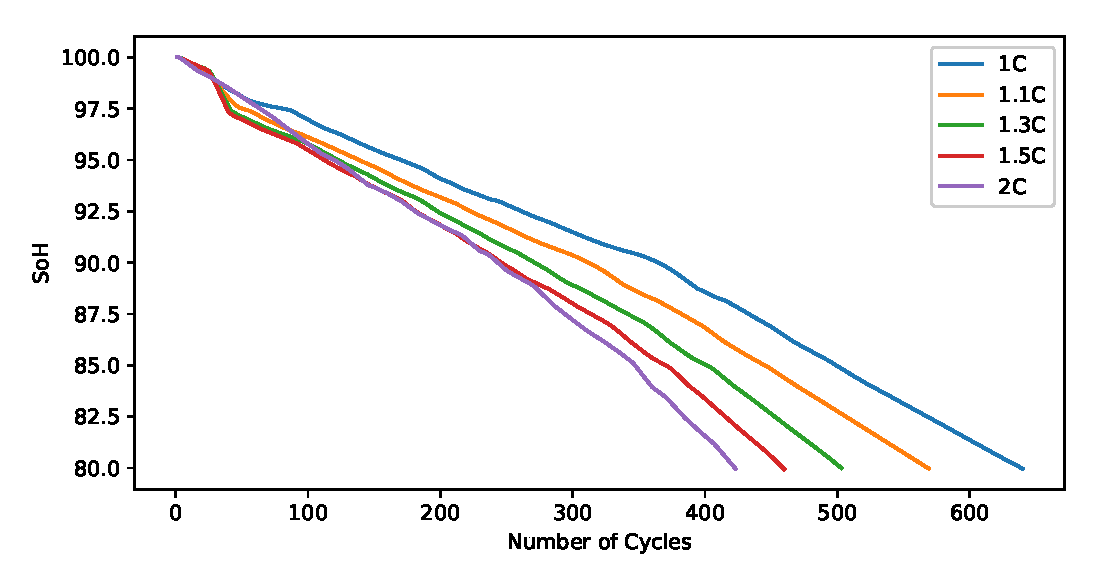
\includegraphics[width=0.7\linewidth]{images/F3_SoH_C.eps}
    \caption{Predicted SoH Degradation Profile for Different Discharge Rates.}
    \label{fig:SoHC1}
\end{figure}
%change axis label to number of full cycles to failure
The battery from the literature was only tested for c-rates between 1C and 2C. However, for the ebike's battery, during the test rides it only experienced an average a drop in SoC of X over around x minutes, resulting in the c-rate for the ebike's battery being about xC. This lays far outside the bounds of the battery model. Though the model could produce a result, the stress factors would be extrapolated and therefore experience disproportional errors. 

The degradation profiles for five discharge rates are shown in Figure \ref{fig:SoHC1}. The specific profile shown in Figure \ref{fig:SoHC1} is unique to the battery, therefore, each specification of battery would display a different SoH profile and also be affected by discharge rate by different amounts.

\subsubsection{Modelling the Effects of Temperature}
%show affect of temperature on the SoH profile of the ebike battery
%show affect of c-rate on the SoH profile of the ebike battery
%show the effect of cycles to failure for different temp and c-rate for ebike battery
\begin{figure}[h]
\centering
\begin{minipage}{.5\textwidth}
  \centering
    \includegraphics[width=0.95\linewidth]{images/F4_cycles_vs_temp.eps}
    \caption{Number of full cycles to failure for different battery temperatures.}
    \label{fig:temp}
\end{minipage}%
\begin{minipage}{.5\textwidth}
  \centering
    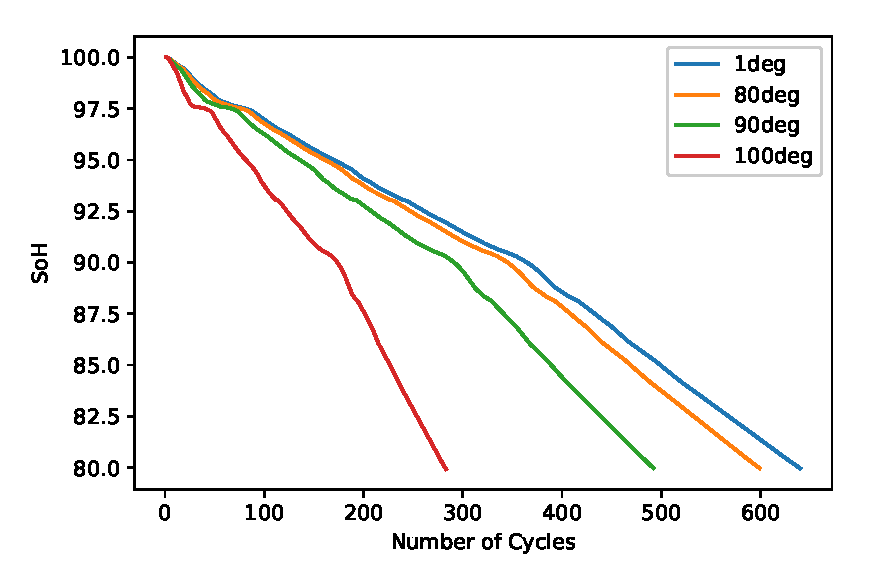
\includegraphics[width=0.95\linewidth]{images/F5_SoH_T.eps}
    \caption{Predicted SoH degradation profile for different battery temperatures.}
    \label{fig:SoHT}
\end{minipage}
\end{figure}

The battery modelled was specified to have an optimal operating temperature range of 0 to 70\textdegree C. This can clearly be seen in Figure \ref{fig:temp} by the sharp drop off in the number of full cycles to failure. This operating temperature is arbitrary as they is no data on it for the ebike battery, however, with enough time, experimental testing could easily be carried out to identify it. Figure \ref{fig:SoHT} shows the effect battery operating temperature has on the degradation profile, stretching the profile significantly in the y-direction as the battery begins to discharge outside of its operational temperature.

\FloatBarrier
\subsubsection{Modelling the Effects of Different Battery Capacities}
\begin{figure}[h]
    \centering
    \includegraphics[width=0.7\linewidth]{images/F6_Cap.eps}
    \caption{SoH Degradation Profile during ebike testing.}
    \label{fig:Cap}
\end{figure}
Changing the capacity of a battery will change its stress factor parameters, therefore, to accurately model different capacities of battery they must first be experimentally tested. However, it would likely be possible to test a sample of the same battery type with different capacities to infer what the stress factor parameters would be for the untested battery capacities. This was not possible in the case of this report, therefore, to demonstrate the effect capacity has on the number of rides until failure it has been assumed that stress factor parameters are constant between different capacities.

Figure \ref{fig:Cap} displays the relationship between the number of cycles to failure and battery capacity. It is important to note that for each battery, the same amount of amp-hours was discharged. Therefore, as battery capacity increase, it has the effect of reducing both the DoD and c-rate. It is therefore beneficial to use a battery that has a larger battery capacity if a product requires a longer battery life. However, increasing the capacity of the battery will have to be weighed against other design factors such as cost, physical size, product lifespan and weight. Depending on the batteries application, each factor would be of different importance, however, once a weighing is applied and battery specifications are know, it would be possible to select an optimal battery.

\FloatBarrier
\subsubsection{Modelling SoH Based on ebike Usage}

\begin{table}[h]
\centering
\begin{threeparttable}
\caption{Estimated conditions experienced by the battery during ebike testing.}
\label{table:condtions}
\begin{tabular}{|c|c|c|c|c|}
\hline
\textbf{Cycle Number} & \textbf{DoD} & \textbf{Pedal Assist Setting} & \textbf{C-Rate*} & \textbf{Battery Temperture (\textdegree C)} \\ \hline
1-10 & 5 & 3 & 1.6 & 15 \\ \hline
11-20 & 20 & 5 & 2 & 20 \\ \hline
21-30 & 25 & 3 & 1.6 & 10 \\ \hline
31-40 & 15 & 2 & 1.4 & 10 \\ \hline
41-50 & 25 & 3 & 1.6 & 15 \\ \hline
51-Failure & 21.25 & 2 & 1.4 & 15 \\ \hline
\end{tabular}
\begin{tablenotes}
\small
\item *C-rate has been scale based on the pedal assist setting to provide values that are usable in the SoH model.
\end{tablenotes}
\end{threeparttable}
\end{table}

To demonstrate the capabilities of the SoH model, data for the test rides of the ebike were estimated and are shown in Table \ref{table:condtions}. For cycle number 51 on-wards, conditions that would be expected of a fleet ebike were input. In the final DT, it would be possible to accurately predict these values based on ebike usage patterns and the predictive dynamics and SoC model. As the usage pattern is not known a constant value was chosen. The impact the test rides would have had on the ebike battery, if it experienced the same SoH profile as the one in the literature, is shown in Figure \ref{fig:SoHcurrent}, and the predictive SoH profile is shown in Figure \ref{fig:SoHpre}. Unfortunately, the number of cycles until failure has little value, as the battery modelled is not the same as the one used on the ebike. However, assuming that the average Santander bike completes 1,039 rides a year \cite{web:bikes} \cite{web:rides}, the model predicts that the battery would need replacing after 4 years and 259 days.

\begin{figure}[h]
\centering
\begin{minipage}{.5\textwidth}
  \centering
    \includegraphics[width=0.95\linewidth]{images/F7_Bat.eps}
    \caption{SoH Degradation Profile during ebike testing.}
    \label{fig:SoHcurrent}
\end{minipage}%
\begin{minipage}{.5\textwidth}
  \centering
    \includegraphics[width=0.95\linewidth]{images/F8_Predic.eps}
    \caption{Predicted SoH Degradation Profile for a fleet ebike.}
    \label{fig:SoHpre}
\end{minipage}
\end{figure}

\FloatBarrier
\subsection{Sensitivity Analysis}
\begin{figure}[h]
\centering
\begin{minipage}{.5\textwidth}
  \centering
    \includegraphics[width=0.95\linewidth]{images/F9_Sen.eps}
    \caption{Predicted Cycles to Failure for Different Battery Temperatures and Discharge Rates.}
    \label{fig:TC}
\end{minipage}%
\begin{minipage}{.5\textwidth}
  \centering
    \includegraphics[width=0.95\linewidth]{images/F10_Sig_Dam.eps}
    \caption{Rate of damage and c-rate stress factor at a SoH of $92.8\%$}
    \label{fig:damage_sigma}
\end{minipage}
\end{figure}

%say how 1.8C and 1.9C is more damaging than 2C and this is because of the limited number of c-rate measured

Figure \ref{fig:TC} shows in detail how both battery temperature and discharge rate affects the number of cycles until failure. One unexpected result from the graph is that discharge rates of 1.8C and 1.9C experience few cycles to failure than 2C. However, this is explained by the method of calculating the c-rate stress factor. The c-rate stress factor is fitted to the experimental data using a second order polynomial curve. However, as can be seen in Figure \ref{fig:damage_sigma} the plot does not always fit the experimental data. This could be due to either experimental error or a second order polynomial not being the most suitable fit for the data. However, it is most likely due to the limited range of discharge rates measured during the experimental testing. The battery found within the literature had only been discharged at five c-rates, therefore limiting confidence of the polynomial curve's fit.

\FloatBarrier
\subsection{Sensor Minimisation}
\textbf{should this still be talked about and should it be in this section????}
Here talk about the trade off between having a current sensor and an accurate model vs predicting current data from Liv and TYs model but a less accurate model

HERE DISCUSS SENSOR SELECTION/REQUIREMENTS

\subsection{Application to Wider DT Technology}
%Product Development Application
%TESTING OF DIFFERENT BATTERY CAPACITIES TO EVALUATE IMPACT (both SOC and SOH)

%Can we say for this case what is the optimum battery size?

%Here discuss that you could take this model one step further to develop a model that outputs an optimum charge/discharge strategy

Batteries are becoming a key technology in modern engineering systems, from electric cars (cite) and aircraft (cite) to large-scale energy storage for integration with the electrical grid (cite). Therefore, being able to model battery degradation presents an opportunity for design optimisation and intelligent operation across a magnitude of industries.

\subsubsection{Design Optimisation}
Without the need of physically testing batteries under the expected designed loads, several batteries could be modelled within the DT to evaluate their performance. Not only could this improve the performance of the battery but it could also reduce the cost and time of testing and significantly reduce the time validation.
In the case of the ebike DT, the dynamics model has been used to predict the power usage over for the lifetime of a fleet ebike, with a distribution of ride lengths and rider abilities that could be expected. Several batteries of different capacities and their respect number of cycles to failure is shown in Figure x. It has been assumed that the batteries experience the same damage coefficient as the reference battery modelled in Figure X, however this is unlikely to be the case, and the damage coefficients would first need to be calculated for each battery capacity. However, the figure does display that there is a trade off to be made between the capacity of the battery and the depth of discharge that would be experience as a result. Knowing the cost of the different batteries, an optimum battery that minimises initial cost and maximises time before it needs replacing could be found.
\\
\textit{put in figure here}

\subsubsection{Testing of Different Batteries for SOC}

SOC results show that for a 45 min ride only 25\% was used therefore could have a much smaller battery on ebike- saves capital costs.

\begin{figure}[H]
    \centering
    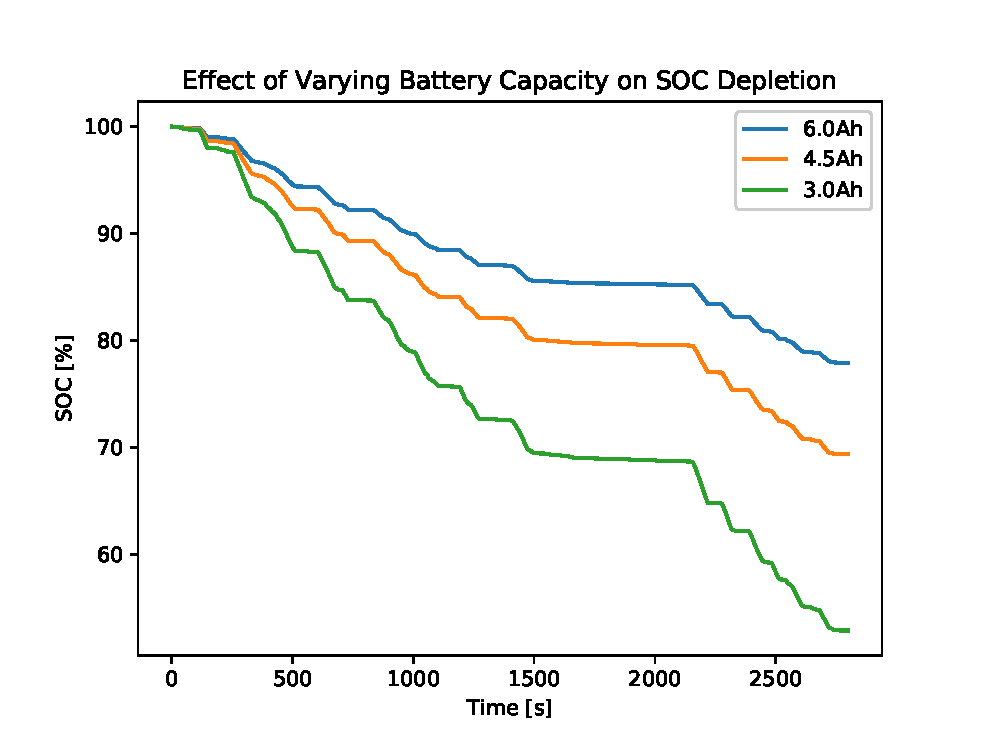
\includegraphics[width=0.6\textwidth]{images/smaller_cap_SOC.eps}
    \caption{A comparison of the effect of varying the battery's capacity on SOC depletion}
    \label{fig:smaller_cap_soc}
\end{figure}

\subsubsection{Intelligent Operation}
%talk about changing usage pattern
Accurately knowing SoH and being able it predict how changes to usage patterns affect it would allow for the operation of the ebike to be altered to best suit the needs of the operator. For example, \textit{implement data from dynamics into the model then talk about how changing usage to be used to extend life or target a set number of uses. also battery degradation is most sensitive later on in its life}.\\
This strategy could be implemented into the offshore wind industry to ensure several wind turbines need maintenance at the same time during periods of reduced wind. Therefore reducing the high cost of dynamic positioning vessel that are required for maintenance. 


\subsubsection{Current Limitations}
%lack of battery data provide by the manufacture. therefore requires each battery type to be tested by the manufacture. therefore though lest testing is needed, physically testing can not be fully negated

There are currently two significant limitations to the implantation of battery SoH models. The first being the limited battery data provided by manufactures, and the second being the lack of understanding of the damage mechanics of battery and how they are affected by changing conditions.
\\

Currently, for the type of model described in this report to be of greatest use, the rate of degradation for different reference conditions must already be known. Otherwise, additional testing is required to find the values oneself, which is costly and time consuming. Being provided with these degradation profiles would, therefore, allow for the easy comparison of batteries without the designer ever needing to physically test the battery.
\\

The issue of requiring prior knowledge of a battery's degradation profile, presented by the use of empirical formula, could be alleviated through the use of analytical models. These would be formulated through understanding the relationship between operational conditions, damage mechanics and SoH. However, the knowledge of these relationships is currently lacking, and without this, these type of models are limited.

\newpage

\section{Model Improvement through Machine Learning Techniques}
\label{sec:Machine_Learning}
A fundamental requirement of a DT is the capability of modelling a system, achieved through mapping a series of input features to a series of outputs, typically through a combination of a set of functions, with the target as producing an output that is as accurate as possible. The work conducted last year focused on building deterministic models, based on interpreting and simplifying the underlying physics of the problem to explicitly define these mapping functions; this allowed for the development of models capable of describing ebike behaviour to an acceptable degree of accuracy. However, aside from sensitivity studies, there was no rigorous method of quantifying the uncertainty within the results. Furthermore, the inflexible nature of the developed models meant they were unable to effectively accommodate any unknown unknowns which, in conjunction with the stochasticity of uncontrollable variables outside of the direct system boundary, occasionally caused significant deviations between predicted results and those observed by the physical product. Furthermore, one of the key conclusions drawn across the previous years' reports was the need for further work in improving the predictive capabilities of the DT models: the ability to accurately predict ebike parameters and thus minimise the frequency of physical testing has been identified both in literature \ref{temp} and by the project partners \ref{temp} are a crucial function for the effective deployment of DTs. Aside from the models' deterministic constraints, the reduced accuracy could be further attributed to the simplifications and assumptions imposed in order to generate the models within the desired time and cost constraints. These issues were highlighted when assessing the predictive capabilities of the Dynamics model, notably the dependency on parametric equations to define to ebike's operating environment: the behaviour of the of the uncontrolled variables influencing the system could not be accurately modelled due to their stochasticity and uniqueness to individual riders. As such, a range of machine learning methods were investigated for their potential in improving the predictive capabilities of the Dynamics model by freeing the model of its underlying deterministic foundations. \medbreak

While the flexibility of machine learning techniques for developing adaptive model architectures has demonstrated rapid uptake across a range of industries, the field of machine learning itself can be broadly classified into three key learning methods \textbf{Need references for the below}:

\begin{itemize}
    \item \textbf{Supervised Learning:} Data sets are manually labelled and features are often manually created. The learning algorithm attempts to learn relationships between the features of given input data and the expected output.
    \item \textbf{Unsupervised Learning:} Data sets have no manually-defined classifications or labels, with the learning algorithm expected to discover underlying patterns and extract features that are not obvious to external observers.
    \item \textbf{Reinforcement Learning:} Typically implemented for goal-oriented problems or tasks, the learning algorithms operates within defined bounds and potential states. Behaviour is subsequently rewarded or penalised with each progressive change in state, encouraging the algorithm to operate using high-reward methods.
\end{itemize}

In order to select an appropriate machine learning model, reformulation of the problem objectives into desired model functionality was necessary and determined as follows:

\begin{itemize}
    \item The ability to accurately predict the performance for current and future assets given a series of inputs. Learning to output a function f: ${\rm I\!R}^n \rightarrow {\rm I\!R} $. 
    \item The ability to flag atypical events to detect performance degradation and/or component failure. 
\end{itemize}

These tasks can broadly be categorised into regression and classification tasks \cite{Goodfellow-et-al-2016} as thus allow for applicaiton to the. 

Due to the exhaustive list of various machine learning techniques, it is necessary to determine a broad class of machine learning models from which a more involved comparison can be conducted. The machine learning techniques proposed below for implementation, while different in function and behaviour, are all suitably categorised as supervised learning models for complex regression problems. These were identified as most appropriate due to the organised and labelled data sets that would be observed during ebike usage.  It should be noted that within the field of machine learning there is no one model that perfectly fits a given application, each method has associated strengths and weakness which must be reviewed in order to select the most appropriate model \cite{SOMETHING ABOUT NO FREE LUNCH}. Table \ref{tab:ML:ML_downselection_matrix} highlights the downselection process in choosing the most appropriate machine learning techniques. The justification for the weightings associated with each evaluation criteria is detailed in Appendix \ref{appendix:Machine_Learning_DS_Justifiaction}.

\begin{table}[h!]
    \centering
    \footnotesize
    \caption{Machine Learning Model Downselection}
    \begin{tabular}{|>{\raggedright}m{0.18\textwidth}|c|>{\centering\arraybackslash}m{0.085\textwidth}|>{\centering\arraybackslash}m{0.085\textwidth}|>{\centering\arraybackslash}m{0.085\textwidth}|>{\centering\arraybackslash}m{0.085\textwidth}|>{\centering\arraybackslash}m{0.085\textwidth}|>{\centering\arraybackslash}m{0.08\textwidth}|}
        \cellcolor{gray!120}\textcolor{white}{\textbf{Evaluation Criteria}} & \cellcolor{gray!120}\textcolor{white}{\textbf{Weighting}} & \cellcolor{gray!120}\textcolor{white}{\textbf{Linear Regression}} & \cellcolor{gray!120}\textcolor{white}{\textbf{Polynomial Regression}} & \cellcolor{gray!120}\textcolor{white}{\textbf{Neural Nets}} & \cellcolor{gray!120}\textcolor{white}{\textbf{Bayesian Inference}} & \cellcolor{gray!120}\textcolor{white}{\textbf{Random Forest}} & \cellcolor{gray!120}\textcolor{white}{\textbf{SVM\tablefootnote{Support Vector Machine}}} \\
        \hline
        \hline
        Minimise Computation Intensity              & 1 & 3  & 3 & 1  & 1 & 1 & 1 \\
        Minimise Bias/Variance Trade-off            & 3 & 3  & 3 & 9  & 9 & 9 & 6 \\
        Maximise Accuracy of Output                 & 3 & 3  & 6 & 9  & 9& 9    & 9 \\
        Minimise Number of Model Hyperparameters    & 2 & 6  & 6 & 3  & 3& 3 & 3 \\
        \hline
        \hline
        Total          &   & 16 & 19& 26 & 26  & 24 & 23 \\
    \hline
    \end{tabular}
    \label{tab:ML:ML_downselection_matrix}
\end{table}

\textbf{This needs to include all of the above for discussion, albeit briefly.} 
A linear regression model makes the assumption that the relationship between $X$ and $Y$ is linear, this is rarely the case in real world applications and therefore unlikely to yield accurate predictions. Polynomial regression can be used to build a more complicated relationship by mapping the $x$ inputs into a higher dimensional "feature space" through a set of basis functions \big($x:\phi (x) $\big). Provided the basis function is fixed, the model is linear in the dimensional space and therefore analytically tractable \cite{rasmussen_williams_2008}. The difficulty then lies in selecting a suitably complex polynomial for the mapping, especially since the underlying function is unknown. Bayesian inference models circumvent this problem by implicitly determining the complexity of the function based on previously observed data however has a significantly greater computational intensity \cite{bishop_2013}.  


\subsection{Data Segmentation}
In order to fully validate the machine learning models it was necessary to ensure that the data used for learning was entirely separate to the data used for testing and validation. The purpose of having a separate testing set is to disincentivise continued tuning of the model to better fit the data following completion, as this could simply be observed as manually correcting the network to perform well on a specific data set, akin to the validation set, and thus non-representative of the network's deployed performance on 'real-world, unseen' data. The data was split into three distinct sets of data as describe in Table \ref{tbl:data_segmentation}. The comparison of training and test data was used to iteratively determine a suitable set of hyperparameters that best captured the underlying mapping between input features and outputs.

\begin{table}[h!]
    \centering
    \small
    \caption{Segmentation of data sets for training, testing and validation.}
    \label{tbl:data_segmentation}
    \begin{tabular}{|c|c|c|}
        \hline 
         \cellcolor{gray!120}\textcolor{white}{\textbf{Data Set}} & \cellcolor{gray!120}\textcolor{white}{\textbf{Size of Data Set}} & \cellcolor{gray!120}\textcolor{white}{\textbf{Data Use}} \\ 
         \hline
         \hline
         Training & 80\% of Train/Test Database & Establish interdependencies between features and outputs  \\ 
         Testing & 20\% of Train/Test Database & Verify interdependencies on untrained observations. \\ 
         Validation & Independent Validation Database & Validate performance for a previously unobserved routes. \\ 
    \hline
    \end{tabular}
\end{table}


%https://www.sciencedirect.com/science/article/pii/S0003267012016479?via%3Dihub -Sample Size

% Robs Refs: 
% https://research.aston.ac.uk/portal/files/117164/NCRG_98_020.pdf

\subsection{Hyperparameter Optimisation} 
\label{sec:Hyperparameter_Optimisation}
To minimise the loss between the observed and predicted outputs of each architecture, it is necessary to appropriately tune individual hyperparameters to optimise model accuracy for the given data set. While this can be done manually, certain machine learning architectures can have up to hundreds of hyperparameters, taking an infeasible amount of time to manually search for the optimal combination. As such, an automated approach is typically incorporated when this finer tuning of hyperparameters are required, as described below.

\begin{itemize}
    \item Brute Force, Grid Search, Random Search, Evolutionary Algorithms, Bayesian Optimisation
\end{itemize}


%%% Neural Net Method %%%
\section{Model Improvement using Neural Network Architectures}
Throughout this section, the implementation of three unique neural network structures is investigated to explore the potential of extending the capabilities of the ebike DT beyond the confines of deterministic modelling. The three key motivations behind each unique network are detailed below:

\begin{enumerate}
    \item Introduction of a new time-prediction methodology to improve on the accuracy of last-year's Dynamics model through utilisation of historic rider data.
    \item Provide a design case for sensor minimisation through inference of voltage signals through raw GPS data. This objective was predominantly motivated through exploration of sensor redundancy in complex and integrated systems, such as within the SOC and SOH models of the ebike, where accurate inference of sensor signal readings reduces the impact severity in the case of critical system failure.
    \item Provide a design case for neural network as a means of sensor redundancy, nominally through signal restoration. This was conducted through the identification and correction of anomolous RPM readings. This objective is motivated by the year 4's Dynamics report \cite{report:dynamics}, where RPM readings were recognised as anomalies following test ride data collection, and had to be manually corrected in post-processing.
\end{enumerate}


\subsection{Background}
Artificial neural networks (ANNs) are computational models taking structural inspiration from the interconnectedness and behaviour of the neuron-synapse anatomy within the brain. While full ANN architectures are typically composed of up to hundreds of neuron-like elementary units, the fundamental behaviour of each artificial neuron is remarkably simple: the neuron takes a set of inputs $\bar{\textbf{x}_j}$ and passes them through some activation function $\Phi (A)$, producing outputs $\textbf{y}_i$. The activation function operates by mapping the inputs and transforming them to some output falling within the range of the function; activation functions must be chosen appropriately for the network architecture being constructed to provide an output in the desired range. Commonly implemented activation functions are shown in Figure \ref{fig:activation_fns}. 

\begin{figure}[h!]
    \centering
    \includegraphics[width=0.55\textwidth]{images/NN_Generic/activation_function.eps}
    \caption{Commonly used activation functions used in ANN architectures.}
    \label{fig:activation_fns}
\end{figure}

The activation function within the artificial neuron lies dormant until a threshold is reached, causing the neuron to 'fire' and provide some output to the next neuron in the network. To determine an appropriate level for the threshold, each input $\textbf{x}_{j}$ is coupled with a weighting, which determines the strength of its influence on the activation function. This encourages inputs that negatively impact the accuracy of the function output to be associated with a low weight, and vice versa for inputs that positively impact the accuracy of the output.\medbreak

The concept of a single neuron can subsequently be extended through concatenation of a number of unconnected neurons to form 'layers', which themselves are stacked to develop full, interconnected neural networks. Figure \ref{fig:combined_ann} demonstrates the structure of an artificial neuron and a combination of such neurons to form a simple ANN architecture. The function of the individual layers is described as follows: the input layer, capturing the inputs, or features, of the data set; the hidden layers, where the bulk of the computation and model optimisation is conducted; and the output layer, providing the network prediction for a given set of inputs.\medbreak

\begin{figure}[h!]
    \centering
    \includegraphics[width=0.7\textwidth]{images/NN_Generic/combined_ann.pdf}
    \caption{(a) Artificial neuron structure; weights are denoted by $w_i$. (b) Simple, fully-connected ANN architecture.}
    \label{fig:combined_ann}
\end{figure}

Within the hidden layers, both the threshold-level and weightings of the activation function are continually fine-tuned and updated through backpropagation of the error of the network output to optimise the model; a well-known example of backpropagation learning rule is the Widrow-Hoff rule \cite{nn:widrow_hoff}, shown in Equation \ref{eq:backprop} below:

\begin{equation}
\label{eq:backprop}
    w_{ij}^{t} = w_{ij}^{t-1} + \eta\delta_i x_j
\end{equation}

$w_{ij}$ represents the neuron weights at time-steps $t$ and $t-1$; $\eta$ represents the learning rate, a hyperparameter defined to limit the rate of convergence; $\delta$ represents the the error between the output groundtruth $y_i^*$ and model prediction $y_i$, thus more precisely defined as $\delta = y_i^* - y_i$; and finally the model inputs $x_j$. This backpropagation optimisation is performed continually during the training phase of a neural network to minimise the observed loss: this phase is one of the three key operational phases of ANN development and deployment. The other two phases are tesing and validation, where the network's performance is compared against unseen data sets, used to identify overfitting to the training data and to provide a theoretical performance baseline for the model's deployment. The key difference between testing and validation data sets is that the former is loss-tested regularly to evaluate performance towards unseen data during training, allowing for fine-tuning of hyperparameters. The latter, however, is tested at the end of the model development when no further changes are to be implemented. The separation of the ebike data sets into these three sets has been covered previously in Section \ref{sec:preprocessing}.

Another benefit of neural networks is that the concatenation of large numbers of non-linear operators provides the ability for application to complex, highly-integrated, technical systems without explicit definition of the fundamental equations that underpin the system itself: they are capable as behaving as universal approximators for any continuous function \cite{nn:universal}. Furthermore, they are capable of application to problems which may not have explicit mathematical solutions, such as image segmentation and classification problems, and are capable of providing solutions to these with seemingly ever-increasing accuracy and speed.\medbreak

However, the ability of universal approximation comes with a caveat: the depth of the network, synonymous with the number of hidden layers, means that the system often operates as a 'black-box', where the interpretation of individual inner operations is difficult and may appear nonsensical when observed in isolation \cite{nn:medical_blackbox_validation}. This often poses the question whether it is possible to place trust in a system that one doesn't fully understand. While the individuality of neural networks for specific problems means there exists no single, formal verficiation and validation method, multiple approaches have been developed across industry leaders. The National Aeronautical and Space Administration identified two key approaches: sufficiently deep modularisation of the network architecture to allow conventional white-box V\&V methods to be suitably applied; and both requirement-driven and design-driven testing, where the network is subjected to in-depth testing to validate output behaviours are as expected, notably outputs at boundary and extreme conditions, correct error handling and recovery, and timing of critical elements within the software code \cite{nn:nasa_blackbox_validation}.

It is for these reasons that neural network architectures have been chosen for exploration to determine any underlying relationships between seemingly abstract feature and output data sets observed during the ebike test ride. Rider cycling behaviours are individually unique and have previously been modelled with the aforementioned determinstic methods. One of the proposed ANN architecture aims to 'learn' underlying rider-cycling behaviours and subsequently extrapolate these to previously unobserved routes. Similarly, the capability to both predict and restore sensor readings across a route was also explored, focussing on the application of neural networks in sensor minimisation through inference from other data sources.

\subsection{Review \& Downselection of Network Architectures}
\label{sec:nn_types}
Over the years, there has been a remarkably consistent stream of 'novel' and 'state-of-the-art' neural network architecture proposals, each demonstrating improvements over predecessors. When developing a neural network for some given problem, the structure is typically constructed using an appropriate baseline configuration identified through literature. However, the ‘ideal’ architecture of a net is unique to each problem, being fundamentally entangled to both the data set and chosen hyperparameters, consequently making it difficult to identify and develop such a structure. As such, given the vast choice of varying network architectures \cite{nn:nn_types}, it was necessary to first reformulate the proposed motivations into appropriate problems for neural networks and then evaluate the appropriateness of generic family architectures. By recognising the time and voltage-prediction problems as complex relationships requiring rider behaviours to be learnt, and the RPM signal restoration as a time-series problem, three key families of network were identified as satisfying the motivations:

\begin{itemize}
    \item \textbf{Multilayer Perceptrons (MLPs)} - Feedforward-only ANN architectures, typically implemented with a relatively small number of fully-connected hidden layers. Deep MLPs include high numbers of hidden layers, and are used to appropriate complex modelling problems. The feedforward nature of these networks indicates that outputs can only pass between subsequent layers unidirectionally and thus each output cannot influence the weights of previous layers.
    
    \item \textbf{Recurrent Neural Networks (RNNs)} - Similar to MLPs, but introduce units that include self-contained loops, mimicking a form of 'memory'. These allow the RNN units to modify any new outputs based on previous outputs from the same unit, introducing the ability for the network to operate on and predict data that requires contextualisation.
    
    \item \textbf{Convolutional Neural Networks (CNNs)} - These networks are commonly used for image classificiation and natural language processing, consisting of convolutional downsampling and upsampling paths within the network \cite{nn:u_net}. However, these can be adapted to time-series framed problems through application of Gramium angular fields (GAFs) to augment the 1D time-series data into 2D, image-like structures for feature extraction through CNNs \cite{nn:gaf}.
\end{itemize}

For investigation into the applicability of neural networks in ebike DTs, the MLP and RNN architectures were determined as most appropriate. While the CNN method has been demonstrated to operate successfully on time-series data \cite{nn:gaf}, the size of the ebike data sets presents the problem of dimensionality when converted from time-series to GAF images: a 1D, time-series dataset of length $N$ increases in dimension to $N^2$ when convered to a 2D GAF. This is further emphasised by ebike routes frequently consisting of over thousands of waypoint recordings, make this approach computationally impractical for fleet-level operations. Furthermore, training on such data sets creates a dependency on inputs of fixed size, creating inflexibile network structures for time-series input data of varying length. As such, this CNN approach was not investigated further in this project.

\subsection{Implementation of the MLP Architecture}
\label{sec:mlp_architecture}
Unique MLP architectures were implemented for the time and voltage-prediction models. The following section details the similar development efforts undertaken across the models. For ease of clarification and depiction of model behaviours where appropriate, a known objective function has been defined to generate demonstration data sets. This example objective function is defined in equation \ref{eq:nn:sine_eq}; note that the network has no observation of the function itself, instead only to samples of the input domain and corresponding outputs. All model validation and discussion is conducted on the observed ebike data, and can be found in Sections \ref{sec:nn:validation} and \ref{sec:nn:discussion}.
\begin{equation}
    \label{eq:nn:sine_eq}
    f(x) =  sin(2.5x) + sin(x) + 10 + \epsilon
\end{equation}

$\epsilon$ is some random noise added to the system. \textbf{TRY AND RERUN THESE WITHOUT USING THIS EQUATION.} The models were developed on the Tensorflow backend in conjunction with the Keras high-level API \cite{nn:tensorflow}. The Keras API was identified as suitable for the development of the neural network architectures, as it's pythonic implementation allows for rapid prototyping while still making full use Tensorflow's powerful graph-based architecture.

%%%%%%%%%%%%%%%%%%%%%%%%%%%%%%%
%%% DATA PREPROCESSING PT 2 %%%
%%%%%%%%%%%%%%%%%%%%%%%%%%%%%%%
\subsubsection{Further Data Preprocessing}

Following initial preprocessing of the raw features from GPS files and creating useful features, as detailed previously in Section \ref{sec:preprocessing}, further data preprocessing techniques were realised as beneficial to network operation and were implemented as such, with the core preprocessing techniques being feature standardisation and data batching. First consider standardisation, otherwise referred to as feature scaling or, more loosely, as normlisation. This technique is often adopted in ANN architectures for multivariate regression problems, involving the scaling of both features and output values to lie within the range of $[-1,1]$; the method for achieving this is demonstrated in equations \ref{eq:nn:midrange} and \ref{eq:nn:standardise}. 
\begin{equation}
\label{eq:nn:midrange}
    midrange = \frac{x_{max} + x_{min}}{2}
\end{equation}

\begin{equation}
\label{eq:nn:standardise}
    \hat{x_{i}} = \frac{x_i - midrange}{\frac{x_{max} - x_{min}}{2}}
\end{equation}

where $x_{max}$ and $x_{min}$ are the maximum and minimum observations of the feature respectively, $x_{i}$ is the value of the feature input, and $\hat{x_{i}}$ is the standardised output returned to the model operator. Standardisation of data is often necessary to allow activation functions to generate appropriate predictions within their output range; an activation function with a range of $[-1,1]$, such as the tanh activation function, would be incapable of mapping an input $x$ to an output $y$ that would nominally lie in the range of $[0,100]$. Further to mapping to viable input and output ranges for the activation functions, data standardisation provides the benefit of removing any initial bias that may occur due to the natural range of the feature values by scaling each individual feature to have the same range. The benefit of standardisation for ebike DT implementation this can be demonstrated through consideration of both gradient and cumulative distance features in making route time predictions: for any given route, the value of the cumulative distance monotonically increases with no inherently imposed upper limit, while road gradients lie within both physical and developmental ranges, with considerably smaller absolute values \cite{nn:hill_gradients}. This widely varying range between the feature inputs may lead to the network architecture being overwhelmed by the dominant feature, in this example the cumulative distance, leading to a phenomenon known as saturation. When saturation occurs, the pre-activation summation of the hidden unit weights within the network rapidly tend to either very large or very small values, resulting in the activation function outputting values at, or very close to, the limits of their output range. Following saturation, small changes in the hidden unit weights become insignificant to the total summation, meaning the network becomes near-incapable of continued learning. In the case of the distance-gradient example, a very high gradient observed by an ebike rider would manifest as a considerably higher required power input, but this relationship may be lost if the network is trained on routes with relatively high cumulative distance, simply due to considerable difference in the absolute values. Saturation can also arise when unnatural interdependencies between features have been developed within the network. This would manifest within the model as the capability of achieving high predictive accuracy for the given training set, but suffering when attempting to generate accurate posterior predictions on previously unseen data, such as that of new ebike routes. As such, the standardisation process removes the potential of unintentional bias, encouraging the network to learn true relationships; however, if a dependence is known ahead of training, this would reflected appropriately within the standardisation process. For the purpose of this model, a naive approach is taken, allowing the model to learn all interdependencies without intervention.\medbreak

The second preprocessing step is the 'batching' of the ebike training data set. Batching involves presenting the network with inputs and features grouped together to form a set of mini-batches, where each mini-batch is a single $M \times N$ array, with $M$ as the batch size and $N$ being the number of GPS features created. A network with a mini-batch size of 1 would result in feeding each feature-output pair to the input layer individually, referred to as a method known as online training \cite{nn:online_learning}. Mini-batching is frequently preferred when the full data set is readily available, as the number of updates to the hidden weights per epoch\footnote{An epoch is defined as the number of times a full training data set is presented to the machine learning model.}, and thus computations, is reduced to \big($n_{samples} / batchsize$\big), down from the $n_{samples}$ computations required when conducting online training. Furthermore, with single batchsize training, the network is subjected to frequent internal covariate shift, where the internal structure of the network is updated on observation of each training sample and thus constantly evolving. This would require low learning rates and suitable parameter initialisation to ensure convergence to the suitable minima and that network saturation did not materialise. To counter this covariate shift phenomenon, the introduction of mini-batching allows for batch normalisation \cite{nn:google_batch_norm} to be implemented, where the activation function of each unit in each layer is presented with a estimated mean and variance by the mini-batch. This normalisation of the activation functions within the network reduces the observed internal covariate shift by providing a distribution across the activation function that is influenced by both the observed mini-batch and full training data set. This consequently reduces the network's susceptibility to irregular hidden weight updates and saturation upon observation of outlying feature points. This is benefical to the ebike DT as it allows the model to accommodate variations in rider behaviour without significantly impacting the capabilities of the predictive model. This would be more influential when the initial fleet size and observed database is small, leading to high variation in riding styles and ebike usage. For example, consider the scenario in which, during early deployment, the majority of the ebikes are used for commutes with relatively low variation in total distance. If a recreational rider were to utilise the ebike for a sufficiently long ride, the fleet-predictive model could become quickly saturated on observation of the new data if trained without batch normalisation. The steps involved in the batch normalisation transform are shown below in equations \ref{eq:nn:batch_norm_mean} to \ref{eq:nn:batch_norm_scale_shift}:
\begin{equation}
    \label{eq:nn:batch_norm_mean}
    \mu_{B} = \frac{1}{m} \sum^{m}_{i=1} x_{i}
\end{equation}

\begin{equation}
    \label{eq:nn:batch_norm_std}
    \sigma^{2}_{B} = \frac{1}{m} \sum^{m}_{i=1} \big(x_{i} - \mu_{b} \big)^2
\end{equation}

where $\mu_{B}$ and $\sigma^{2}_{B}$ are the mean and variance of the mini-batch with size $m$. $x_{i}$ are the feature observations contained within the mini-batch. The mini-batch observation can then be normalised across the full data set:

\vspace{-0.5em}
\begin{equation}
    \label{eq:nn:batch_norm_normalise}
    \hat{x}_{i} = \frac{x_{i} - \mu_{B}}{\sqrt{\sigma^2_{B} + \epsilon}} 
\end{equation}

where $\hat{x}_{i}$ is each normalised observation in the mini-batch and $\epsilon$ is a small value added to avoid zero-division instabilities. Finally the normalised output is scaled and shifted by hyperparameters $\gamma$ and $\beta$ respectively:

\begin{equation}
    \label{eq:nn:batch_norm_scale_shift}
    y_{i} = \gamma\hat{x}_{i} + \beta
\end{equation}

A demonstration of the effects of batch normalisation are depicted in Figure \ref{fig:nn:batch_normalisation}. Note that the model run with batch normalisation implemented converges over 50 epochs before the non-implemented model, both using the same model hyperparameters. Furthermore, with journey data would be collected and processed post-ride as opposed to being conducted in real-time, the implementation of mini-batching would be more computationally, and thus cost, efficient while concurrently reducing susceptibility to the hindering effects of internal covariate shift. \medbreak

\begin{figure}[h!]
    \centering
    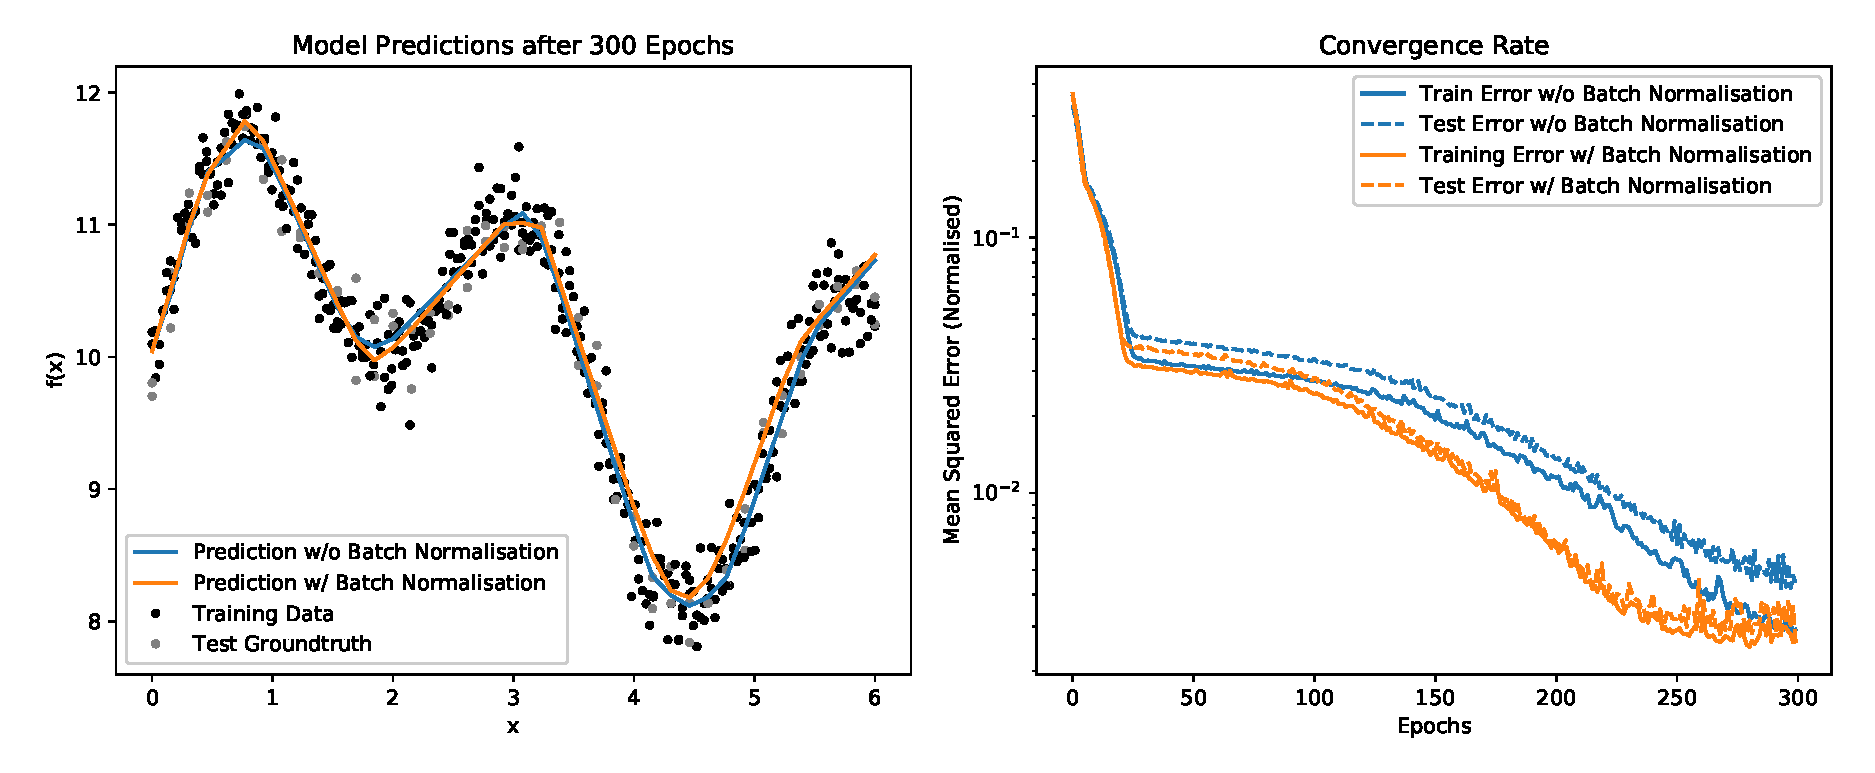
\includegraphics[width=\textwidth]{images/NN_ANN/batch_normalisation.eps}
    \caption{Demonstration of the effects of batch normalisation on the objective function defined in equation \ref{eq:nn:sine_eq}.}
    \label{fig:nn:batch_normalisation}
\end{figure}

Another regularisation technique implemented across all architectures was the inclusion of 'dropout' \cite{nn:dropout}. To reduce the likelihood of unnatural co-dependencies being developed between units within the network, and thus encouragement of network overfitting to the training data, the dropout technique gives each unit in every layer, both input and hidden layers alike, a probability $P_{drop}$ of being removed from the network ahead of training. This creates a network with randomly connected nodes across the layers, forcing the model to learn generalisation of behaviours from the data set, and not simply learning the observed inputs; dropout has been shown to be an highly effective technique in regularisation for improving test set accuracies. A depiction of a network with dropped units is shown in Figure \ref{fig:nn:dropped_nn}, and a demonstration of the effects on training and testing error shown in Figure \ref{fig:nn:dropped_demo}. As a design consideration, this function was integrated within the model architectures to prevent overfitting to historic rider data, and allow the network to make appropriate and accurate predictions for both new routes and riders alike.  \textbf{TODO: Run model w/ current params to gen dropout data.} 

\begin{figure}[h!]
    \centering
    \includegraphics[width=0.3\textwidth]{images/NN_Generic/dropout.pdf}
    \caption{Depiction of a network experiencing unit dropout; the dropped units are crossed through.}
    \label{fig:my_label}
\end{figure}

%%%%%%%%%%%%%%%%%%%%%%%%%%%%%%%%
%%% HYPERPARAMETER SELECTION %%%
%%%%%%%%%%%%%%%%%%%%%%%%%%%%%%%%
\subsubsection{Hyperparameter Selection}

Following data preprocessing, the next step was the selection of model hyperparameters that allowed for timely convergence to a local minima of each of the applied problems. The hyperparameters identified for implementation within the MLP are described and tabulated in Table \ref{tab:nn:generic_hyperparams}, including values for the time-prediction architecture included; the unique sets of hyperparameters for each model are fully captured in Appendix \textbf{APPENDIX HERE}. \medbreak

\begin{table}[h!]
    \centering
    \small
    \caption{Hyperparameters for the MLP, with the values as used for the time-predicting network architecture.}
    \begin{tabular}{|c|c|c|}
        \hline 
         \cellcolor{gray!120}\textcolor{white}{\textbf{Hyperparameter}} & \cellcolor{gray!120}\textcolor{white}{\textbf{Description}} & \cellcolor{gray!120}\textcolor{white}{\textbf{Example Values}} \\ 
         \hline
         \hline
         Epochs & Times to run the full training data set through the model. & 2000  \\ 
         Learning Rate, $\eta$ & Rate of descent for the optimiser. & 1$e^{-5}$  \\ 
         Learning Decay, $\mu$ & Rate of decay of the descent rate. & 1$e^{-10}$  \\ 
         Dropout, $P_{drop}$ & Probability of unit to be dropped from network. & 0.1  \\ 
         Mini-Batch Size, $m$ & Size of data mini-batch. & 1024  \\ 
         N$^{o}$. Hidden Layers & Number of hidden layers. & 5  \\ 
         N$^{o}$. Units & text Number of units per hidden layer. & 250  \\ 
        \hline
    \end{tabular}
    \label{tab:nn:generic_hyperparams}
\end{table}

Due to project constraints with regards to both time and computational power, no self-optimising hyperparameter algorithm was implemented to determine a global minima for the model. The main limitations with regards to computational power arise from both the ebike training data sets ranging up to hundreds of thousands of data points in combination with the necessity of operating across nine individual hyperparameters, and then attempting to conduct this optimisation on inadequate hardware. While certain hyperparameters could be fixed to reduce the number of dimensions to conduct the optimisation within, such as the number of epochs and mini-batch size, this would likely lead a local minima and not necessarily be the most efficient solution. A potential method would be to restrict the absolute training time, but this directly depends on the number of unique data points and feature instances in the data set. As such, optimisation methods should be explored with the availability of increased computing power. Due to dimensional complexity of visualising optimisation of all hyperparameters, a simplified, uni-dimensional depiction of the optimisation of the 'epoch' hyperparameter is demonstrated in Figure \ref{fig:nn:sine_epochs}, where increasing the value of the epoch hyperparameter correlates to a decreasing mean squared error for this particular model structure.

\begin{figure}[H]
    \centering
    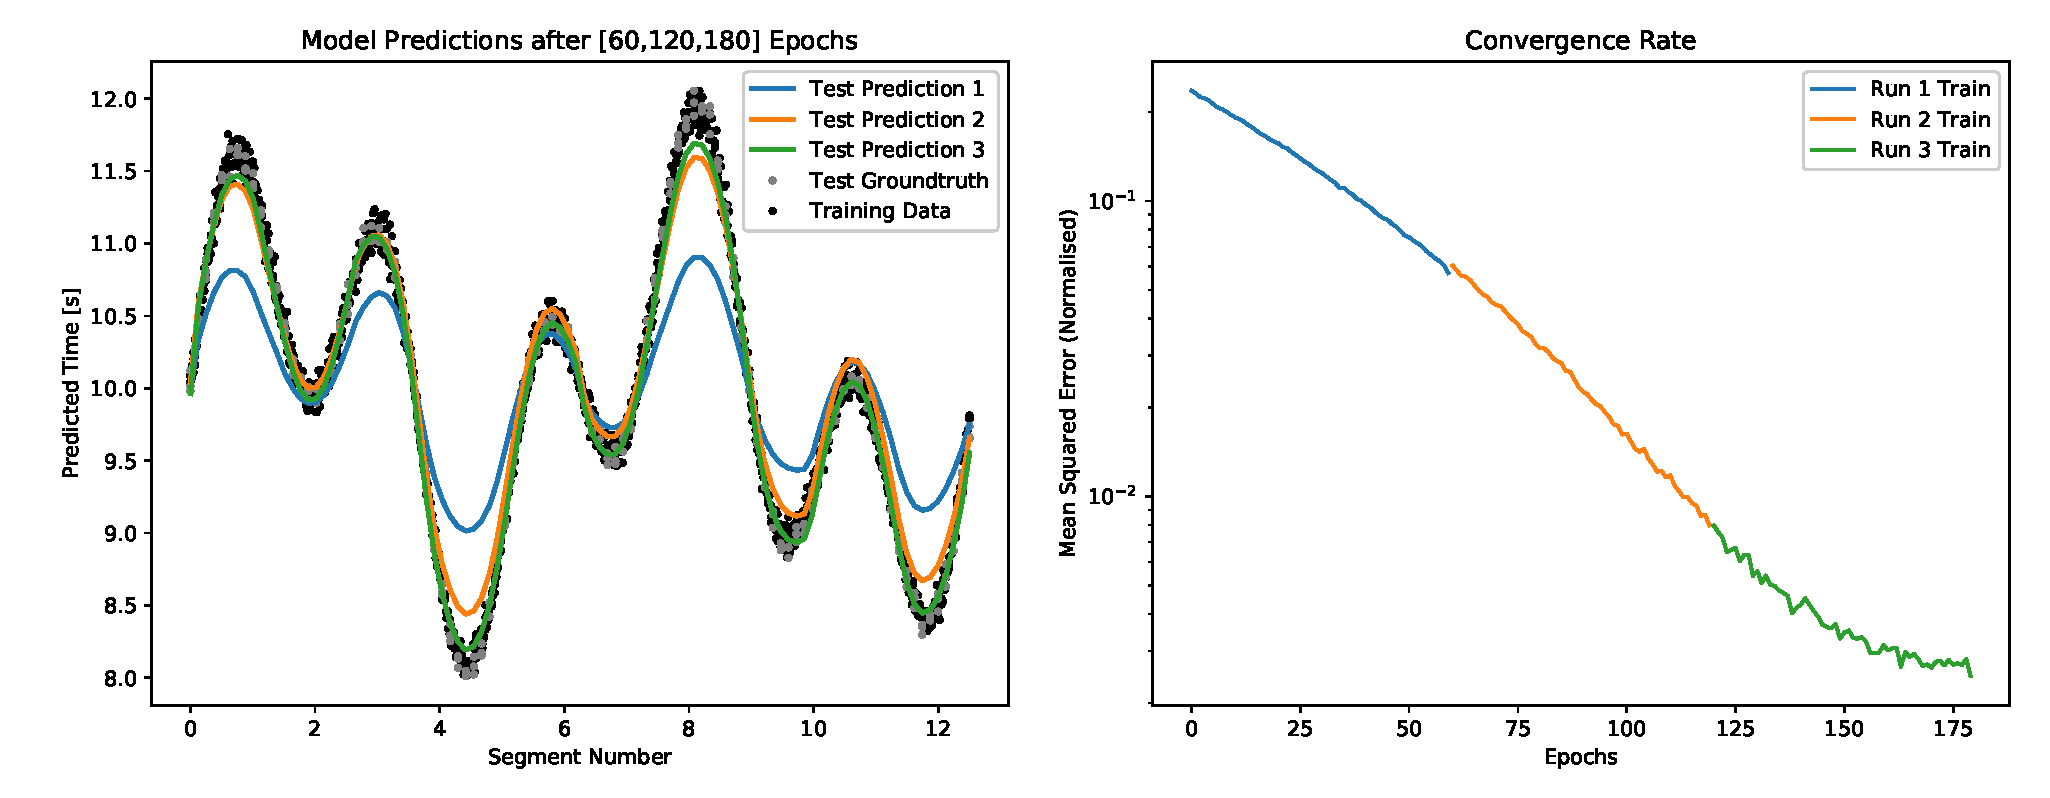
\includegraphics[width=0.99\textwidth]{images/NN_ANN/sine_epochs.eps}
    \caption{Demonstration of accuracy of a given model structure improving with increasing number of trained epochs on.}
    \label{fig:nn:sine_epochs}
\end{figure}

However, it should be noted that the stochastic nature of neural networks means that it is near-impossible to get identical model behaviour on subsequent runs. Part of this is reliant on the internal complexity of the network structure during training, in conjunction with random initialisation of the hidden unit weights and biases. As such, it is possible to conduct multiple model runs with some tending to the right solution, while others suffer from early convergence in a local minima. This is more commonly exhibited in complex models training with low quantities of data or with too high a training rate, as there are a considerable number of potential solutions that fit the training points. The stochastic nature of the network is depicted across three individual model runs providing uniquely different results is shown in Figure \ref{fig:nn:sine_stochastic}. Further discussion about the stochastic behaviour of neural networks and how this can be mitigated on integration to critical ebike systems can be found in Section \ref{sec:nn:discussion}.

\begin{figure}[H]
    \centering
    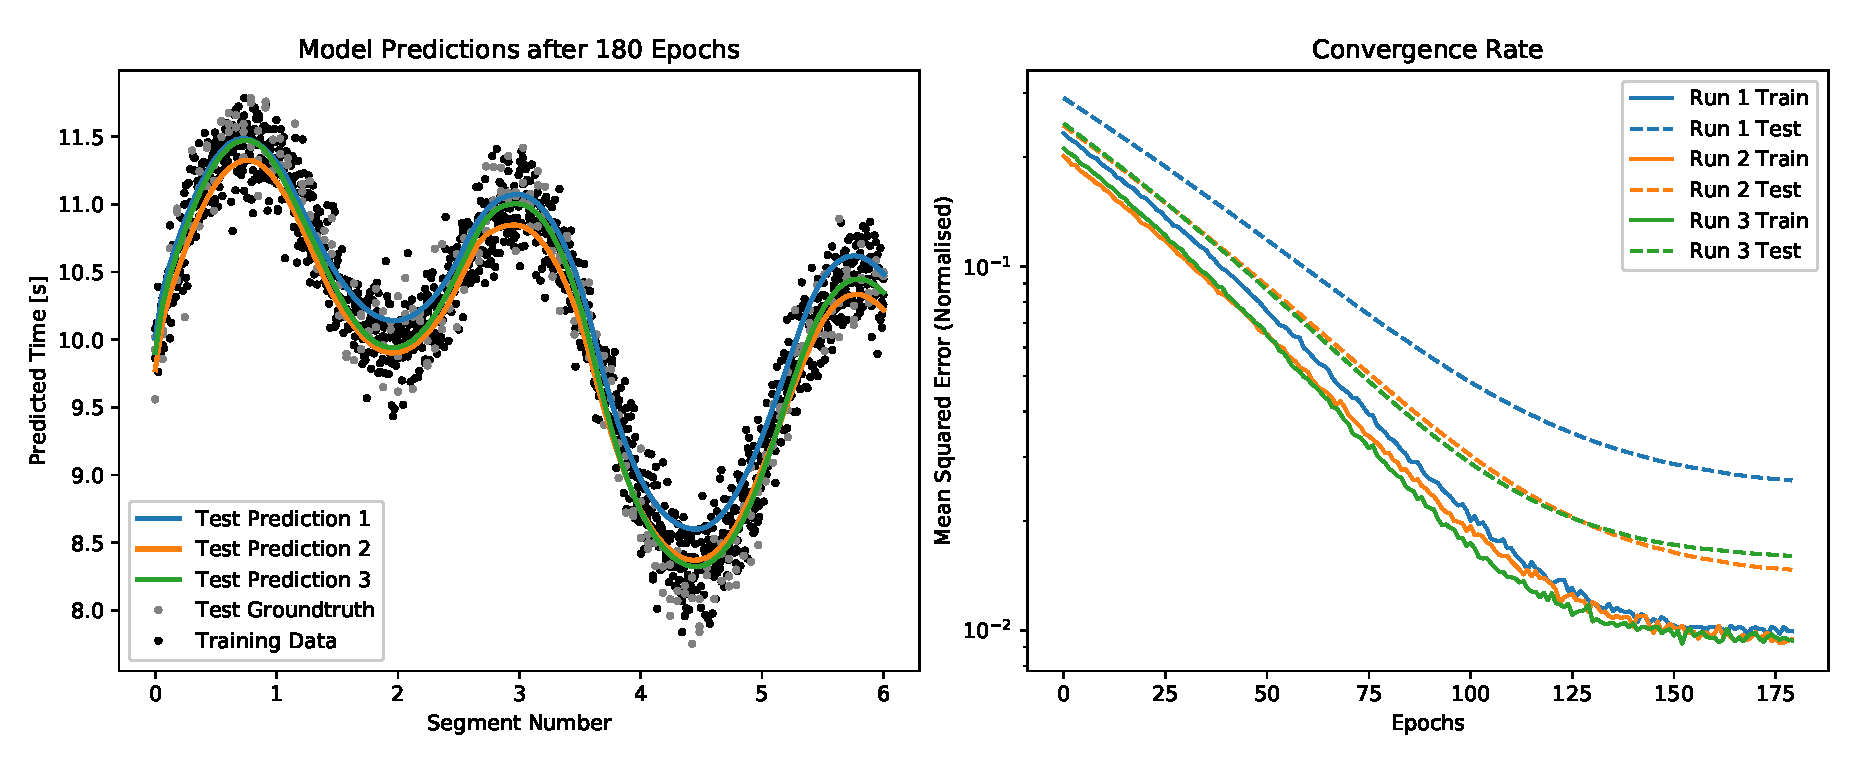
\includegraphics[width=\textwidth]{images/NN_ANN/sine_stochastic.eps}
    \caption{Demonstration of the stochastic nature of the neural network architecture when trained on a noisy objective function, as defined in equation \ref{eq:nn:sine_eq}. The MLP was trained in three individual instances, each providing a unique mapping output.}
    \label{fig:nn:sine_stochastic}
\end{figure}

%%%%%%%%%%%%%%%%%%%%%%%%%%
%%% OPTMISER SELECTION %%%
%%%%%%%%%%%%%%%%%%%%%%%%%%
\subsubsection{Internal Model Optimiser}

The last integral part of model development is the implementation of the network optimiser algorithm and corresponding loss function. The Adam optimiser is a commonly used optimiser for stochastic functions, capable of adaptive learning rates and navigating out from low-gradient optimisation spaces through utilisation of exponentially decaying averages of the historic gradients \cite{nn:adam_optimiser}. The computations carried out by the Adam optimiser are described as in equations \ref{nn:adam_mt} to \ref{nn:adam_vt}. Initially, the first and second moments, $m_{t}$ and $v_{t}$ respectively, of the gradient $g_{t}$ of a stochastic objective function at timestep $t$ are determined:
\begin{equation}
    \label{nn:adam_mt}
    m_{t} = \beta_{1} m_{t-1} + (1 - \beta_{1})g_{t}
\end{equation}
\begin{equation}
    \label{nn:adam_vt}
    v_{t} = \beta_{2} v_{t-1} + (1 - \beta_{2})g_{t}^2
\end{equation}

with $\beta_{1}$ and $\beta_{2}$ are decay rate constants of 0.9 and 0.999 respectively. To operate against a bias tending towards zero during the initial timesteps, the following correction is applied:

\begin{equation}
    \label{nn:adam_mt}
    \hat{m_{t}} = \frac{m_{t}}{1 - \beta_{1}^{t}}
\end{equation}
\begin{equation}
    \label{nn:adam_vt}
    \hat{v_{t}} = \frac{v_{t}}{1 - \beta_{2}^{t}}
\end{equation}

Finally, the Adam update step of the model parameters can be computed:

\begin{equation}
    \label{nn:adam_update}
    \theta_{t} = \theta_{t-1} - \alpha \frac{\hat{m_{t}}}{\sqrt{v_{t}} - \epsilon}
\end{equation}

where $\theta_{t}$ and $\theta_{t-1}$ are the models parameters at timesteps $t$ and $t-1$ respectively. $\alpha$ and $\epsilon$ are the gradient stepsize and a numerical stability constant respectively. Like with the optimisation of model hyperparameters, the model optimiser must also be chosen appropriate to the network architecture and problem at hand. The Adam optimiser is an efficient method of minimising the mean squared error loss function for regression problems experiencing high high noise, and has thus been chosen for implementation across all network architectures throughout this project.\medbreak


%%%%%%%%%%%%%%%%%%%%%%%%%%
%%% RNN IMPLEMENTATION %%%
%%%%%%%%%%%%%%%%%%%%%%%%%%
\subsection{Implementation of the RNN Architecture}
The overall design approach for RNN implementation followed a similar structure to that of the MLP network, but with a fundamental change to the core operating units of the network to accomodate the RPM restoration motivation. Only novel or significant modifications for the RNN architecture are detailed in the following section, otherwise similar internal functions from the MLP implementation can be assumed to have been appropriately adapted to fit this network.

%%%%%%%%%%%%
%%% LSTM %%%
%%%%%%%%%%%%
\subsubsection{The Long Short Term Memory Network}
As a subset of the RNN family, Long Short Term Memory networks (LSTMs) develop on the original internal looping behaviour of simple RNNs, instead forming unqiue 'memory cells' with improved historic influence on unit weights and biases; the elementary structure of one of these cells is depicted in Appendix \ref{NEED_REF}. The arrangement of each cell allows for the LSTM network to learn both long and short-term dependencies within the weights and biases by viewing historic output information to make improved predictions. The potential of this unique structure was realised notably for real-time anomaly detection and signal restoration applications, both of which are demonstrated on RPM sensor readings in Section \ref{sec:nn:results}.\medbreak

\subsubsection{Further Data Preprocessing}
For development of LSTM architecture, a significant modification to the preprocessing step was required to structure the data correctly for training the LSTM network on historic data, in addition to the previously detailed data normalisation. The method implemented was the 'sliding-window' technique, an alternative to the batching method identified previously, where batches instead overlap across the input data to form 'windows', with each window looking back $t$ time-steps in the time-series data and subsequently used to predict the next step $y_{t+1}$. While similar to the aforementioned data batching, an underlying difference in the windowing method is the inclusion of previous prediction groundtruths in predicting the output for the next time-step: this is the root of the memory within the LSTM network, using previous instances of outputs to estimate where the next value will lie. By utilising this unique 'lookback' hyperparameter, model predictions are no longer based solely on ebike data observations at single time steps and, instead, historic observations can now be used to influence predictions. This was recognised as beneficial for this particular problem, as the ebike RPMs demonstrates relatively smooth variation over time, and are not as prone to an erratic and spontaneous external input from the rider, such as input power. The implementation of the sliding-window operation is illustrated in Figure \ref{fig:nn:windowing}.

\begin{figure}[h!]
    \centering
    \includegraphics[width=0.7\textwidth]{images/NN_Generic/windowed_data.pdf}
    \caption{Illustration of the data windowing operation, with $lookback = 2$. Note that the generic sliding-window groundtruth mapping is as follows: $y_{i} = x_{i+lookback}$.}
    \label{fig:nn:windowing}
\end{figure} 

An overview of the complete ANN architecture logic and operation is depicted in the flow diagram Figure \ref{fig:nn:mlp_flowchart}:

\begin{figure}[h!]
    \centering
    \includegraphics[width=\textwidth]{images/NN_Generic/MLP_structure.pdf}
    \caption{Flowchart demonstrating general MLP and LSTM architecture operation.}
    \label{fig:my_label}
\end{figure}


%%%%%%%%%%%%%%%%%%%%%%%%%
%%% MODEL ASSUMPTIONS %%%
%%%%%%%%%%%%%%%%%%%%%%%%%
\subsection{Model Assumptions}
In order to allow for suitable development and deployment of the network achitectures, a number of assumptions were made about the underlying ebike system and data collection methods used.

\vspace{0.5em}
\textbf{Rider Journey-Time Prediction}
\begin{itemize}
    \item Manual definition of input features from raw latitude-longitude-elevation coordinate trios is a valid method of providing insight into more specific route details, such as segment distance and gradient.
    \item There exist underlying, complex relationships within the extracted training feature and output sets that capture rider behaviours across a route.
    \item The recorded ebike data is sufficiently accurate to act as groundtruth inputs within the model.
    \item Any behavioural rider mappings captured by the network are trained on a sufficiently large and diverse data set to prevent overfitting, and thus extrapolated to demonstrate the feasibility of representing overall trends that would be captured at both fleet and individual rider-levels.
\end{itemize}

\textbf{Rider Journey-Current Prediction}
\begin{itemize}
    \item The absolute distance between subsequent coordinate trios is sufficiently small to allow for linear interpolation to be used when aligning against data from sources at higher sampling rates. This allows for linear acceleration equations of motion to be employed to model behaviour route segment behaviours at a finer level.
\end{itemize}

\textbf{Signal-Restoration}
\begin{itemize}
    \item The rear-wheel RPM values identified as anomalous in the previous year's testing phase were validly identified as anomalous through hand calculations; full methodology can be found in last year's Dynamics report \cite{report:dynamics}.
\end{itemize}


%%%%%%%%%%%%%%%%%%%%%%%%%%%%%%%%
%%% KEY FINDINGS AND RESULTS %%%
%%%%%%%%%%%%%%%%%%%%%%%%%%%%%%%%
\subsection{Neural Network Outputs \& Results}
The following section briefly details key outputs from the developed models. Methods of model validation and further results discussion can be found in Sections \ref{sec:nn:validation} and \ref{sec:nn:discussion} respectively.

\subsubsection{Rider Journey-Time Prediction}
Figures \ref{fig:nn:time_pred_r1}, \ref{fig:nn:time_pred_r2} and \ref{fig:nn:time_pred_r3} demonstrate MLP's predicted segmental and cumulative times for three individual riders, with comparison between training on full fleet data and the previous year's Dynamics model time-prediction method for the same. The same fleet model is used to generate each rider's prediction, with the route taken between riders remains consistent.
\begin{figure}[h!]
    \centering
    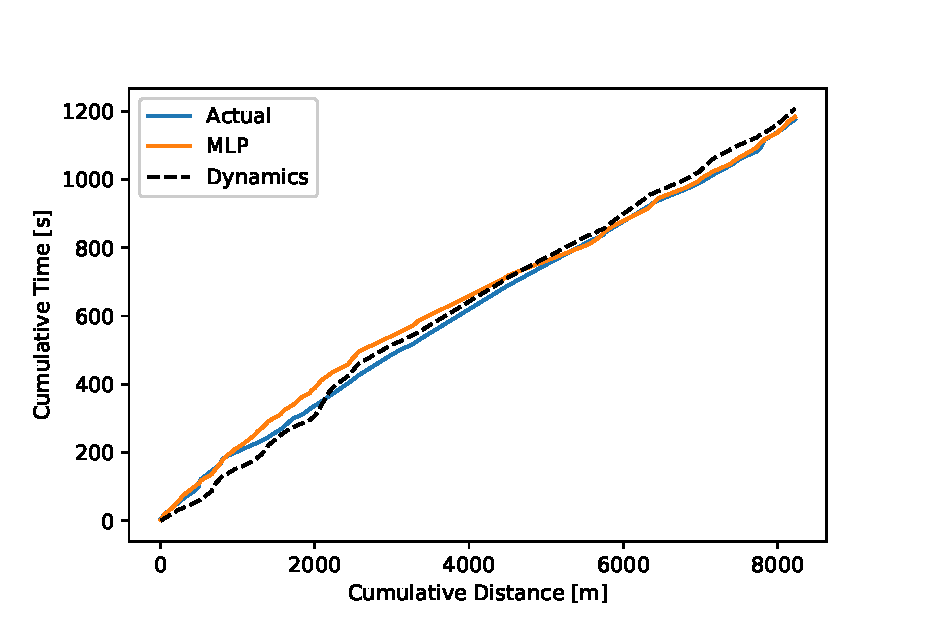
\includegraphics[width=0.6\textwidth]{images/NN_TestRide/CM_Cumulative_Time.eps}
    \caption{MLP time prediction for Rider One, trained using historic fleet data.}
    \label{fig:nn:time_pred_r1}
\end{figure}

\begin{figure}[h!]
    \centering
    \includegraphics[width=0.6\textwidth]{images/NN_TestRide/RR_Cumulative_Time.eps}
    \caption{MLP time prediction for Rider Two, trained using historic fleet data.}
    \label{fig:nn:time_pred_r2}
\end{figure}

\begin{figure}[h!]
    \centering
    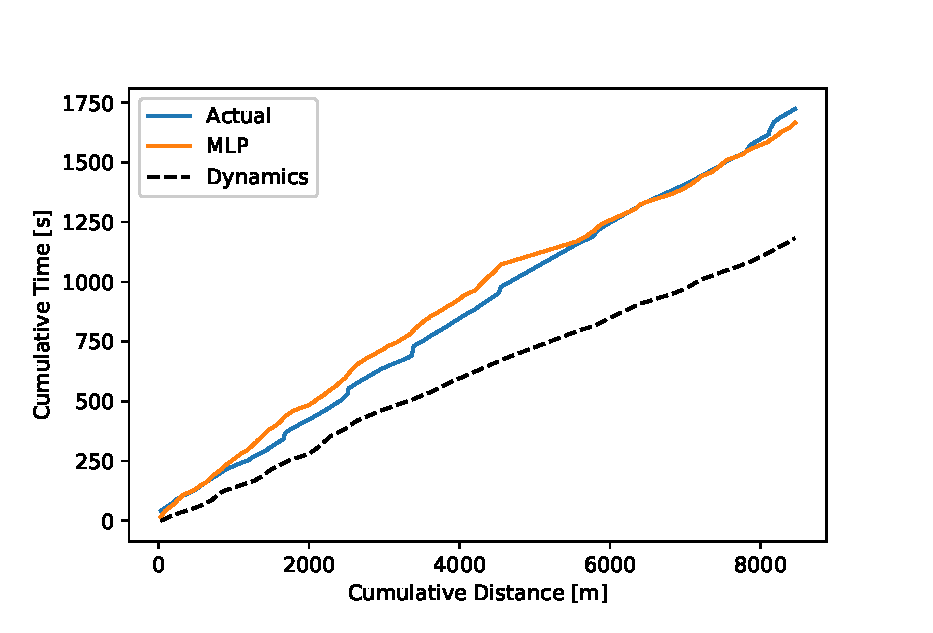
\includegraphics[width=0.6\textwidth]{images/NN_TestRide/OD_Cumulative_Time.eps}
    \caption{MLP time prediction for Rider Three, trained using historic fleet data.}
    \label{fig:nn:time_pred_r3}
\end{figure}

\subsubsection{Journey-Voltage Predictions}
In utilising post-ride GPS data to infer voltage readings, MLP predictions for two individual routes are captured in Figures \ref{fig:nn:current_pred_1} and \ref{fig:nn:current_pred_2}. Note that the voltage readings are converted into current using a nominal resistance as identified in Section \ref{sec:SOC}. This allows predictions to be fed directly in the SOC model, simplifying model integration and allowing the SOC model to view the ANN model simply as a representative current signal. In the segmental current draw predictions, the ANN model accurately predicts key trends over time, but typically underestimates the groundtruth observations. Considering Figures \ref{ref} and \ref{ref}, the model demonstrates strong agreement with the total cumulative current draw: this is key when considering the SOC depletion, as the total current draw correlates significantly with the final SOC state.
 
\begin{figure}[h!]
    \centering
    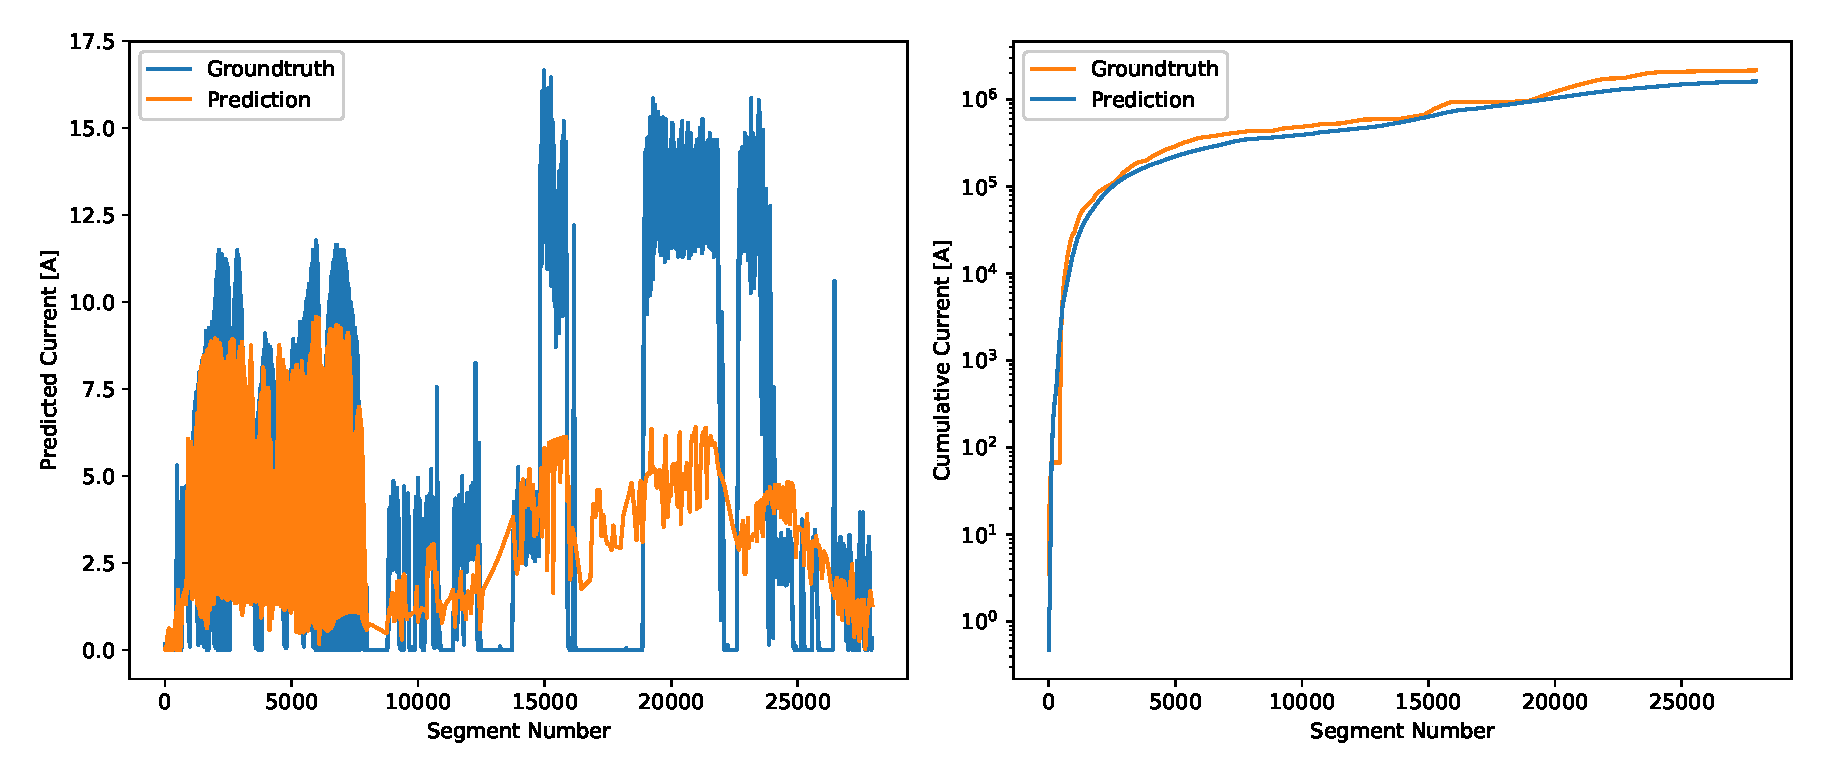
\includegraphics[width=0.95\textwidth]{images/NN_ANN/current_pred_short.eps}
    \caption{MLP current prediction.}
    \label{fig:nn:current_pred_1}
\end{figure}

\begin{figure}[h!]
    \centering
    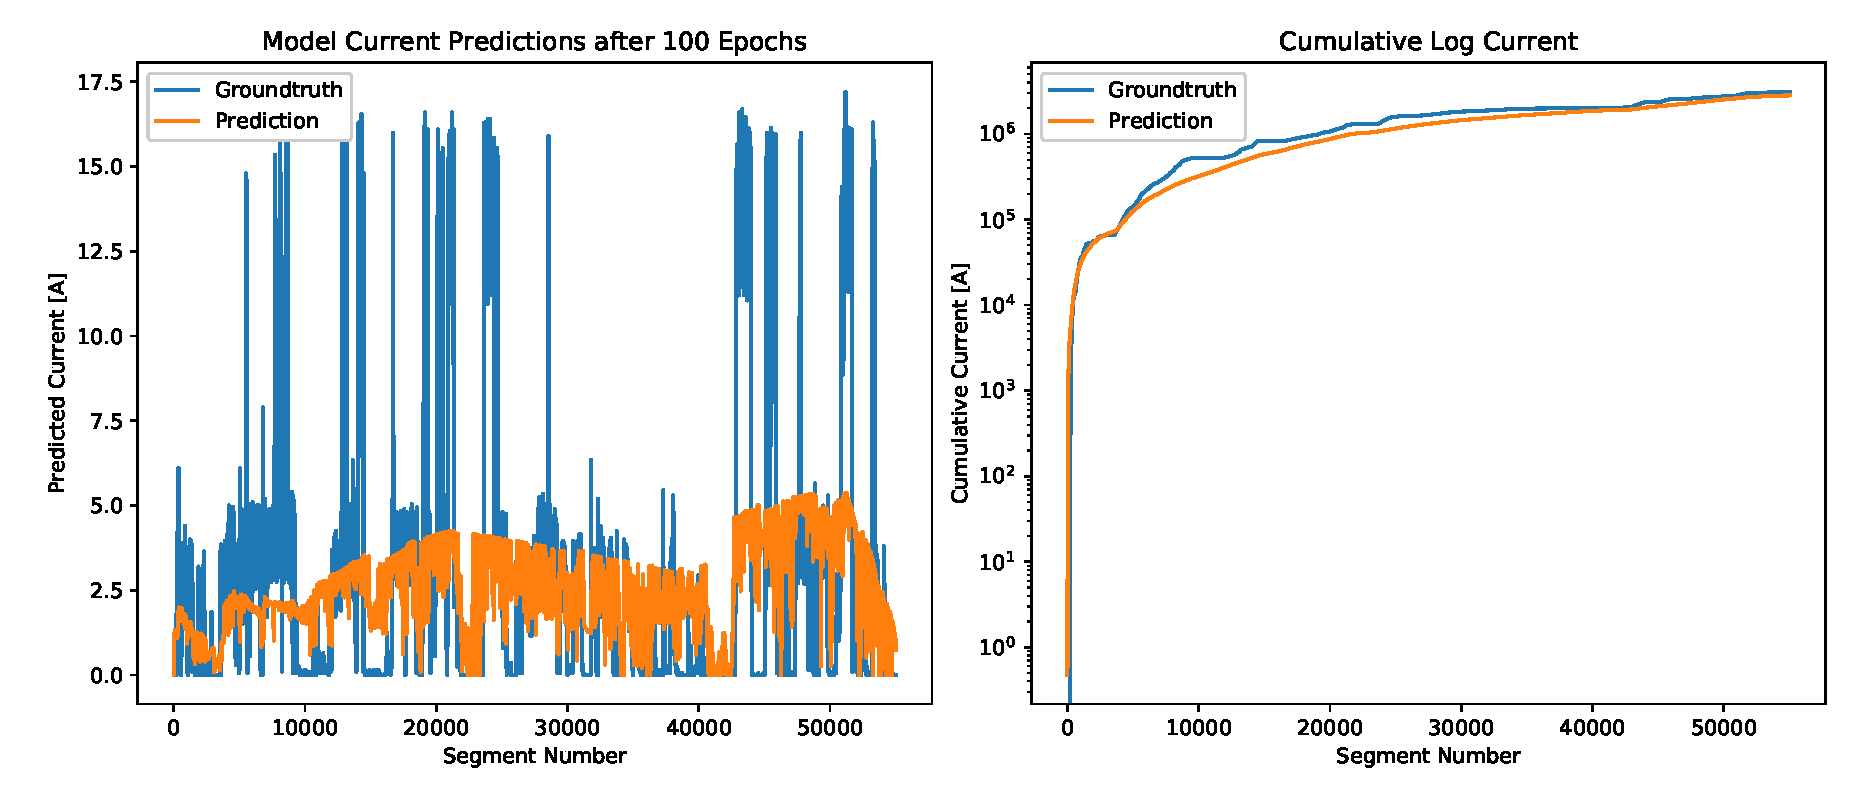
\includegraphics[width=0.95\textwidth]{images/NN_ANN/current_pred_long.eps}
    \caption{MLP current prediction.}
    \label{fig:nn:current_pred_2}
\end{figure}


\subsubsection{Anomaly Recognition \& Signal Restoration}
Figure \ref{fig:nn:lstm_anom} demonstrates the LSTM network's predictions in identifying and restoring trends on previously unobserved RPM observations. To provide some insight into the inner workings and effectiveness of the LSTM architecture, the full set of training data of which the LSTM has previously observed is shown: this demonstrates the LSTM's ability in determining underlying trends with little prior context.

\begin{figure}[h!]
    \centering
    \includegraphics[width=0.9\textwidth]{images/NN_LSTM/lstm_find_anomalies.eps}
    \caption{Text here.}
    \label{fig:nn:lstm_anom}
\end{figure}

%%%%%%%%%%%%%%%%%%%%%%%%
%%% MODEL VALIDATION %%%
%%%%%%%%%%%%%%%%%%%%%%%%
\subsection{Model Validation}
\label{sec:nn:validation}
Throughout model development, considerable care and attention was kept in ensuring the model behaved as expected, particularly during implementation of data preprocessing and network regularisation techniques. To validate such techniques were integrated correctly, model performance was evaluated across multiple runs before and after implementation of the new function: comparing the observed variation in response against supporting literature aided in confirming new behaviours were as expected. Previously shown Figures \ref{fig:nn:batch_normalisation}
and \ref{fig:nn:dropout} demonstrate examples of this validation methodology.

Further care was taken in ensuring that the model behaved with consistency, and that any high-performing architectures were not the result of fortunate stochastic behaviour. Such behaviour would be inappropriate in a complex, technical system where consistently accurate predictions are fundamental to system operation, most notably if implemented at a fleet-operation level, where highly-stochastic predictive capabilities could have significant, and potentially negative, influence on operator reputability and running costs. As such, validation of model stability was conducted through a high-quantity of repeated training runs on both identical model structures and training data, before observing the mean and standard deviation of a number of result metrics for the predicted outputs. This provided insight to ensure that the models were not prone to architectural instabilities and predicted results were not highly varied. Figures \ref{fig:nn:time_pred_r1}, \ref{fig:nn:time_pred_r2} and \ref{fig:nn:time_pred_r3} depict the variation of time predictions of low-epoch training. For each rider, three unique predictions are given based on 20 relatively quick and separate training runs: this was conducted to validate that the stochastic nature of the developed ANN would not dominate and either present significantly varied predictions, or deviate considerably from the groundtruth. As evident in the figures, despite being presented with low quantities of training data and epochs, the model maintains stability and demonstrates a tendency to overpredict rider velocities. A further summary of stability metric results conducted on this MLP architecture can be found in Table \ref{tab:nn:time_mean_std}.

 \begin{figure}[h!]
    \centering
    \includegraphics[width=0.95\textwidth]{images/NN_ANN/time_pred_r1.eps}
    \caption{Text here.}
    \label{fig:nn:time_pred_r1}
\end{figure}

 \begin{figure}[h!]
    \centering
    \includegraphics[width=0.95\textwidth]{images/NN_ANN/time_pred_r2.eps}
    \caption{Text here.}
    \label{fig:nn:time_pred_r2}
\end{figure}

 \begin{figure}[h!]
    \centering
    \includegraphics[width=0.95\textwidth]{images/NN_ANN/time_pred_r3.eps}
    \caption{Text here.}
    \label{fig:nn:time_pred_r3}
\end{figure}

\begin{table}[h!]
    \centering
    \small
    \caption{Model stability metrics across 20 unique training instances of an identical model.}
    \begin{tabular}{|c||c|c|c|}
        \cellcolor{gray!120}\textcolor{white}{\textbf{Metric}} & \cellcolor{gray!120}\textcolor{white}{\textbf{Rider One}} & \cellcolor{gray!120}\textcolor{white}{\textbf{Rider Two}}& \cellcolor{gray!120}\textcolor{white}{\textbf{Rider Three}}\\
        \hline
        \hline
        Mean $\mid$Segmental Difference$\mid$ & 16.800 & 32.824 & 37.177 \\
        St.Dev. $\mid$Segmental Difference$\mid$ & 0.616 & 0.281 & 2.668 \\
        \hline
        Mean $\mid$Cumulative Difference$\mid$ & 58.000 & 209.928 & 335.910 \\
        St.Dev. $\mid$Cumulative Difference$\mid$ & 19.699 & 35.426 & 51.836 \\
        \hline
        Mean $\mid$Segmental Mean Squared Error$\mid$ & 6.937 & 15.593 & 17.440 \\
        St.Dev $\mid$Segmental Mean Squared Error$\mid$ & 0.628 & 2.182 & 1.873 \\
        \hline
    \end{tabular}
    \label{tab:nn:time_mean_std}
\end{table}

Considering the voltage prediction architecture, the output was passed through the SOC model, detailed in Section \ref{sec:SOC}, to further validate against the experimental SOC retrieved from the observed current data. As evident in Figure \ref{fig:nn:soc_ML}, there is strong correlation between the experimental SOC depletion curve and that predicted using the ANN architecture. While further experimental testing and data collection would be required to fully validate the performance of the voltage prediction capabilities, there is sufficient evidence to indicate that the potential for signal inference using a distinctly separate data is feasible and should be explored further.

 \begin{figure}[h!]
    \centering
    \includegraphics[width=0.6\textwidth]{images/NN_ANN/soc_ML.eps}
    \caption{Text here.}
    \label{fig:nn:soc_ML}
\end{figure}

For the signal restoration architecture, a similar method of repeated model training was conducted to ensure consistent model performance. Due to the low quantities of training data necessary to complete more rigorous validation tests on the data against all model types, the model architectures were subjected to performance testing using the experimental objective function defined in equation \ref{eq:nn:sine_eq}.

 \begin{figure}[h!]
    \centering
    \includegraphics[width=0.95\textwidth]{images/NN_LSTM/lstm_nofind_anomalies.eps}
    \caption{Text here.}
    \label{fig:nn:lstm_no_anom}
\end{figure}

 \begin{figure}[h!]
    \centering
    \includegraphics[width=0.95\textwidth]{images/NN_LSTM/lstm_overfind_anomalies.eps}
    \caption{Text here.}
    \label{fig:nn:lstm_overanom}
\end{figure}

%%%%%%%%%%%%%%%%%%%%%%%%
%%% MODEL DISCUSSION %%%
%%%%%%%%%%%%%%%%%%%%%%%%
\subsection{Discussion of Results}
\label{sec:nn:discussion}
\subsubsection{MLP's for Rider Journey-Time Prediction}
As demonstrated in Figures \textbf{Ref}, the ANN model developed for predicting rider journey times is capable of providing accurate estimates based solely off of data collected at a fleet level, despite operating with a relatively limited data set across few riders. While the individual rider predictions using each test set are remarkably accurate, one should be wary that while route used for test set are different to all training routes, the riders used to gather data over these routes have been the same. While this demonstrates the model's strong capability of learning rider behaviours and making predictions for a new journey, it should be cautioned that a previously unobserved rider was not available to truly determine the predictive abilities for a novel rider. However, the distribution between the three test riders was significant enough to observe three distinct journey completion times for the test route, with the model capable of predicting the journey times with an average of \textbf{ERROR VAL HERE} error. It should also be noted that the model is likely to have been limited by not just the availability of fleet and rider-level data, but also by the computational power required to develop an 'optimum' network for the problem; this is true across all of the developed architectures. Access to more capable hardware, in tandem with model refinement to operate efficiently on said hardware, may have introduced scenarios where the model accuracy could be improved on from that developed, simply through non-manual optimisation of the network hyperparameters and structure.

Further studying Figures \ref{fig:nn:time_pred_r1} to \ref{fig:nn:time_pred_r3}, it is clear where the model struggled to pick up some key segmental times, leading to deviation of the cumulative prediction form the groundtruth. Typically, the model underpredicted times at certain segments of the journey; this can most likely be attributed to external conditions that impacted the rider's ability to continue with their journey, such as coming to traffic lights at an intersection or a congested road. This is most clear in Figure \ref{fig:nn:time_pred_r2} around segment 87, where the model failed to accurately predict an approximately 35s segment. Cross-checking this position with the Strava positional map 

\subsubsection{MLP's for Sensor Inference \& Minimisation}


\subsubsection{LSTM's for Signal Anomaly Recognition \& Restoration}
 As clear in Figure \ref{fig:nn:lstm_anom}, the LSTM was capable of identifying anomalies in observed data and correcting the predictions accordingly. Using only two previous routes for prior training, both of which are noticeably different and relatively short. The threshold-based anomaly detection operated in real-time and synchronously with the LSTM's predictions, thus allowing values labelled as anomalous to be dropped from the model's sliding-window and replaced with the previous prediction. This permitted the network to restore the curve and minimise the impact of anomalous sensor values.

%%%%%%%%%%%%%%%%%%%%%%%%
%%% FUTURE WORK %%%
%%%%%%%%%%%%%%%%%%%%%%%%
\subsection{Future Development}



%%%%%%%%%%%%%%%%%%%%%%%%
%%% Gaussian Process %%%
%%%%%%%%%%%%%%%%%%%%%%%%
\section{Model Validation using the Gaussian Process (GP)}
\label{sec:GP_WholeSection}
\begin{comment}
Using GP to model SOH of Li Batts \cite{article_Zhenpo_Wang}


\begin{itemize}
    \item Mathmatical Understanding 
    \item Prior Assumptions encoded by kernals 
    \item Optimal Experimental Design 
\end{itemize}

WHY PICK GP 




\begin{itemize}
    \item The posterior distribution can be computed exactly in closed form
    \item Possible to compute marginal likelihood of the observed data given the model, enabling model comparison. 
    
\end{itemize}
LIMITATIONS 
\begin{itemize}
    \item Exact Inference is slow for large datasets however this can be resolved through approximate inference \cite{DBLP:journals/corr/HensmanFL13}. 
    \item GP scales poorly as the number of observations $N$ increases. 
    \item Must select a suitable kernel
\end{itemize}
\end{comment}

The Gaussian process can be used to assess non-linear functions that map inputs (features) to outputs, where: the form of the function is unknown; the function is known but difficult to compute analytically; or it is costly to obtain the data to determine the specific function parameters. A high level overview of modelling using the Gaussian process is defined in Appendix \ref{appendix:gp_explained}. Accurately defining this function enables future predictions to be made based on a new set of features. As discussed previously the physics based deterministic models created last year were not capable of accurately making these predictions and so a more robust approach was required. The Gaussian process uses a non-parametric Bayesian approach to infer the underlying function. This method is beneficial compared with parametric modelling since the complexity of the function is implicitly determined from the observed data, defining a prior probability distribution over the functions directly. Utilisation of the GP is extremely powerful since a Gaussian distribution has infinite support. Therefore it is statistically possible for any function to be represented and thereby uncover the true mapping of the inputs to outputs even if they are unknown to the creator of the model, enabling a continuous improvement for future predictions \cite{Williams97predictionwith}. The downside to this is that the process can become very computationally expensive since the domain space can become infinitely large as the data set increases. In order to reduce the computational burden and amount of data required to build a suitable model, a non zero mean can be used to place significant bias in a given area of the domain space where the model creator believes the mapping is likely to lie, namely a prior belief. The closer this prior belief fits the data the less data required to create a high confidence model, discussed further in Section \ref{sec:NonZeroMean}.


\subsection{Mathematical Derivation}

The Gaussian process is a prior over the function $p(f)$ which can be used for Bayesian regression (Equation \ref{eq:GP_bayes})

\begin{equation}
    \label{eq:GP_bayes}
    p(f|D) = \frac{p(f)p(D|f)}{p(D)}
\end{equation}

The Gaussian process can be defined as a collection of random variables which follow a jointly Gaussian distribution \footnote{For the Gaussian process the random variables are the evaluation of $f(x)$ at an input location $x$}. Assuming the underlying function can be defined by Equation \ref{eq:gp_mapping} where $\epsilon$ is the associated error defined as $\mathcal{N}(0,\sigma_\epsilon^2)$. A Gaussian process is entirely defined by Equation \ref{eq:GP-definition} where $m(x)$ represents the expected function given the inputs x and $k(x,x')$ defines the covariance function (kernel). The kernel defines a distribution over functions from which samples can be drawn at any number of points.


\begin{equation}
    \label{eq:gp_mapping}
    y = f(\mathbf{X})+ \epsilon
\end{equation}


\begin{equation}
    \label{eq:GP-definition}
    f(x) \sim \mathcal{GP}(m(x),k(x,x'))
\end{equation}



In order to make predictions for a set of inputs, $X_*$ based on a set of previously observed data points $y_t = f(X_t)$. The function $f_*$ must be drawn from the posterior distribution: $p(f|X_t,y_t)$, where $f_*$ follows a joint multivariate normal distribution as defined in Equation \ref{eq:GP_joint_multivariate}. In order to sample from the Gaussian process an input vector of theoretically infinite length is used. The outputs at these locations are then drawn from the multivariate normal distribution created from the kernel. The covariance between each point in the input vector is computed ($K(X_*,X_*)$. The computational cost of this calculation is significantly reduced through use of a zero mean. The observed data's associated noise $\epsilon$ is accounted for by the $\sigma_{\epsilon}$ on the diagonal of the covariance matrix. This is due to the fact that the noise is independent of the underlying function. 


\begin{equation}
    \label{eq:GP_joint_multivariate}
    \begin{bmatrix}
           y_{t} \\
           f_{*} \\
         \end{bmatrix} 
          \sim \mathcal{N}
    \Bigg( 0, \begin{bmatrix}
           K(X_t,X_t) + \sigma_{\epsilon}^2\mathbf{I} & K(X_t,X_*) \\
           K(X_*,X_t) & K(X_*,X_*) \\
         \end{bmatrix} \Bigg)
\end{equation}


\subsection{Application to Electric Bikes}

The Gaussian process was utilised to accurately predict the time required to complete a randomly defined journey for a given rider. Accurate prediction of this information enabled models such as SOC ( Section \ref{sec:soc_dynamics_modeldev}) and power/energy modelling (Section \ref{sec:Dynamics_Development}) to perform with increased accuracy. Furthermore the process of creating a GP model is transferable to other applications and once proved as a concept for time predictions can be re-designed for directly modelling SOC/SOH of an ebike. 


\begin{table}[h!]
\caption{Assumptions for the GP}
\label{tbl:GP_Assumptions}
\begin{tabular}{|p{0.45\textwidth}|p{0.45\textwidth}|}
\hline
Assumptions & Validity \\ \hline
The time required to conduct a journey is independent 
of the cumulative journey time.                     &   The average rental time of a bike in London was 19 minutes                                                             between 2010-2018 and so fatigue effects are likely to be negligible \cite{tfl}           \\
The gradient across a journey segment is constant   & Initial journey segments are small. \\
A rider's weight is a suitable way to categorise riders & There is a strong correlation between fitness and weight  \cite{}. Whilst not entirely accurate, defining more features would increase the computational costs and so a compromise must be made\\
    
\hline
\end{tabular}
\end{table}


The Gaussian Process is well suited to resolving regression style problems as is the case here and was utilised to improve the predictive capabilities of the physics based dynamics model, both for real and theoretical users, whilst incorporating additional benefits such as: confidence intervals, fault tolerance detection and sensor minimisation. Whilst this section will focus on the application to the ebike industry the process and implementation is transferable to any industry/ application through redefining the model features/parameters and will be discussed further in Section \ref{sec:DT_technology}. The features used to define a GP model can be divided into two broad categories, asset features and operating features. The asset's features remain constant throughout the entire life span and can then be utilised to formulate predictions about future products: In the application of electric bikes, asset features could be a rider's weight. By passing in all of the data previously collected from riders of known weights into the Gaussian model, a prediction and confidence interval of the new riders expected time can be produced. This prediction could be made more accurate, given enough data by creating a more complex asset feature space for example by considering a riders stature and perceived fitness level\footnote{Whilst this is subjective, given enough data an underlying trend can still be uncovered}. The operating features define the environment that the product is subjected to. In the application of ebikes examples include, journey distances, gradients and proximity to corners. The number of features determines the dimensionality and therefore size of the domain space.
The application of the Gaussian Process to this scenario operates in a 5 dimensional space and therefore cannot easily be depicted graphically.

\subsection{Design Approach}

Figure \ref{fig:GP_flow} displays the design process undertaken for creating the GP model. The sub-models require independent validation, as defined in Table \ref{tbl:GPsubmodel_validation}, before being integrated and validated as a whole as specified in Figure \ref{fig:v_model}.

\begin{figure}[h!]
    \centering
    \includegraphics[width=\textwidth]{images/GP_Flow_Diagram.eps}
    \caption{Flow Diagram for Gaussian Process}
    \label{fig:GP_flow}
\end{figure}




\begin{table}[]
\caption{Submodel Validation for GP Model}
\label{tbl:GPsubmodel_validation}
\begin{tabular}{|l|l|} \hline
Model                    & Validation Method                                                                                                             \\ \hline
Prior Dynamics Model     & Validated last year. Improvements to the model are independently validated in Section \ref{sec:Dynamics_Development}             \\
Real Data                & Sensor Validation Conducted last year \cite{report:dynamics}. \\
Zero mean Adjusted GP    & Evaluation of known 1D case, where performance can be explicitly quantified (Appendix \ref{appendix:gp_explained})                                                  \\
Hyperparameter Selection & Comparison against alternative methods including brute force method/grid search \\ \hline                                              
\end{tabular}
\end{table}


\subsection{Kernel} 
\label{sec:kernel}
A Kernel \footnote{A Kernel or covariance function is a positive-definite function of two inputs $x_i$ and $x_j$} used for a Gaussian process encodes all of the assumptions made surrounding the function's form and specify which functions are more likely given a prior belief of the functional form. For this application an assumption is made that there is a high correlation between outputs if the distance between two feature inputs $x_i$, $x_j$ is small whilst points far away in the input space are uncorrelated. In the application of ebikes this is to say for example that if the difference between two journey segment distances is small, the expected time to complete each of these journey segments will be similar. This assumption is encoded using a squared exponential kernel (Equation \ref{eq:kernel_squared}) where the hyper-parameters are defined as:
\begin{itemize}
    \item $l$ - Length Scale - dictates the smoothness of the function and defines the region over which it is safe to extrapolate. 
    \item $\sigma$ - Signal Variance - sets the criteria for defining outliers. 
    \item $\sigma_{noise}$ - Predicted Noise - Defines the expected noise and therefore dictates the size of the confidence interval.
\end{itemize}

\begin{equation}
    \label{eq:kernel_squared}
    k(x_i,x_j)= \sigma^2exp \bigg(-\frac{(x_i-x_j)^2}{2l^2} \bigg)+ \delta_{ij}\sigma_{noise}^2
\end{equation}

Kernels can be combined together through addition and multiplication to create a kernel with the desired properties required for a given application. In the application of ebikes, a multi-dimensional kernel is required to enable parameterisation of several distinct features. This can be achieved by multiplying several individual kernels, one for each given dimension. Equation \ref{eq:kernel_seard} shows the multi-dimensional variant of the squared exponential kernel (Squared Exponential Automatic Relevance Determination) where $D$ indicates the number of dimensions (feature) \cite{duvenaud}. Assigning and learning a length scale for each individual feature implicitly defines the significance of that dimension \cite{neal_1995}. This can be used to assist in sensor minimisation procedures. Where the length scale is very large, implies that the feature bears little relevance on the measured output, suggesting them model can perform to a similar level without use of this information and therefore the sensor used to record this information is not required. Calculating the covariance function using this kernel function is computationally expensive and the computational burden increases exponentially with the number of features. An alternative approach is to standardise the data and use the squared exponential kernel (Equation \ref{eq:standardise}) however, this process is unable to identify the significance of individual features since one length scale is used to define all of the input features. Table \ref{tab:kernel_computation} summarises the difference in computational cost when using each kernel function for a fleet database. This computation becomes particularly significant during hyperparameter optimisation because of the iterative nature of the optimisation. Due to the significant increase in computational time for ARD kernels, the use of such kernels was limited to the model design stages when assessing the suitability of features. After which a SE kernel was used with standardised data. The relative difference in performance for the two methods was negligible as shown in Appendix \ref{appendix:kernel_compare}. This gives further validity for the use of Type II ML when determining optimal hyperparamters, since the use of different kernels yielded different results for optimal hyperparameters whilst both methods performed to an equivalent standard.


\begin{table}[]
    \centering
    \begin{tabular}{|c|c|} \hline
    
        Kernel & Average Computation Time [s]  \\ \hline
        Squared Exponential  & 12.2  \\ \hline
        Squared Exponential Automatic Relevance Determination (ARD)  & 124  \\ \hline
    \end{tabular}
    \caption{Computational Cost of Kernels}
    \label{tab:kernel_computation}
\end{table}

\begin{equation}
    \label{eq:kernel_seard}
    k(x_i,x_j)= \sigma^2exp \bigg(-\sum_{d=1}^D \frac{(x_{id}-x_{jd})^2}{2l_d^2} \bigg)+ \delta_{ij}\sigma_{noise}^2
\end{equation}




\begin{equation}
    \label{eq:standardise}
    z= \frac{x-\bar{X}}{\sigma}
\end{equation}

https://stats.stackexchange.com/questions/362511/how-to-use-the-squared-exponential-kernel-with-multidimensional-vector-inputs


DISCUSSION OF NON STATIONARY KERNEL FUNCTIONS


Suitable selection of hyper-parameters is vital in creating a GP capable of making accurate predictions. For large numbers of hyper-parameters the methods discussed in Section \ref{sec:Hyperparameter_Optimisation}. However, for the GP, only a small number of parameters require optimisation ($l$, $\sigma$ and $\sigma_{noise}$) and therefore the simplest method to implement is a maximisation of the log likelihood function (Type II Maximum Likelihood) (Equation \ref{eq:ML}) through gradient based methods \cite{Fletcher:1987:PMO:39857}. The determinant is smallest when the matrix $C_N$ is diagonal and therefore type II ML will favour a smoother function (large length scale). This process also favours a larger $\sigma^2$ which prevents overfitting and therefore is a more effective method than simply minimising the absolute difference between the observed and predicted outputs. Figure \ref{fig:gp_brute} shows the results from performing a grid based brute force optimisation for all three hyperparameters. The smooth nature of these surfaces confirms the use of gradient descent based methods for optimisation.   



\begin{equation}
    \label{eq:ML}
    ln (p(t|\theta)) = -\frac{1}{2} \bigg( ln(|C_N|) +Y_t^TC_N^{-1}Y_t + \frac{N}{2}ln(2\pi) \bigg) 
\end{equation}


\begin{figure}[H]
\centering
\begin{subfigure}[b]{.33\textwidth}
  \centering
        \includegraphics[width=\textwidth]{images/GP_Brute/l_scale_noise_sigma_0.eps}
\end{subfigure}%
\begin{subfigure}[b]{.33\textwidth}
  \centering
        \includegraphics[width=\textwidth]{images/GP_Brute/sigma_noise_l_scale_0.eps}
\end{subfigure}
\begin{subfigure}[b]{.33\textwidth}
  \centering
        \includegraphics[width=\textwidth]{images/GP_Brute/l_scale_sigma_noise_0.eps}
\end{subfigure}%
\caption{Effect of Hyper Parameter Variation on Log Maximum Likelihood}
\label{fig:gp_brute}
\end{figure}


Table \ref{} summarises the results from the hyperparamteter optimisation. The optimisation was repeated for a series of random initialisation, this ensured that the global minimum was found.   

\subsection{Noisy Observations}

The level of noise when observing data can be used to define a confidence interval for future predictions, accurately defining the confidence interval can be used to determine whether or not future data is considered to be anomalous or influence the overall mapping (Error Classification). [REF THIS].

\subsection{Reducing Computation Time}
\label{sec:NonZeroMean}
One disadvantage of the GP is that since any mapping function is statistically possible, large amounts of data are often required and the analysis can therefore become computationally expensive due to the curse of dimensionality \cite{bishop_2013}. The amount of data required can be reduced by encoding structure through use of kernels which can help to construct model's with a larger degree of interpretability. 


A zero-mean enables inference to be conducted using solely the kernel function, significantly reducing the computational cost of the process. The number of data points and therefore computational cost required for the Gaussian Process to converge to the correct solution can be further reduced through use of a suitable prior belief. To implement a non zero mean, the prior belief is subtracted from all observations as defined in Equation \ref{eq:GP_non_zero}. After conducting the Gaussian Process the mean values are then added on to define the true mapping.

\begin{equation}
    \label{eq:GP_non_zero}
    k(x,x')= {\rm I\!E}[(f(x) - m(x))(f(x') - m(x))]
\end{equation}



\subsection{Results}


Analysis was undertaken to understand the amount of training data required to formulate accurate predictions for a rider's journey under differing prior beliefs. A zero mean prior belief was used as a baseline to compare alternative prior models: the dynamics model created last year \cite{report:dynamics} and the second iteration of the model (Section \ref{sec:Dynamics_Development}).Random subsets of training data of varying sizes from the fleet database were taken and used to predict a specific test ride defined in Appendix \ref{appendix:Strava_Test_Ride}. The performance of the GP is partially dependent on how evenly spread out the training data is over the domain space as explained in Appendix \ref{appendix:gp_explained}, therefore the test was repeated twenty times and the predictions averaged. Figure \ref{fig:GP_converge_cum_tim} displays the results. As the number of training points increases the performance of the GP improves for all three prior beliefs. The relative difference in performance between each prior decreases since the GP becomes more reliant on observed data and less reliant on the prior beliefs. The complexity of the problem is significantly greater than the case of the 1D sine wave and the observation error is much larger, therefore a larger number of training samples are required in order for the model to yield accurate predictions. The models tend towards 

This enables justifications for the expenditure on modelling to be justified. When the cost of data collection is difficult/ expensive a prior belief with high accuracy that may cost more to develop is justifiable. If however, the cost of data collection is relatively low the demand for a more accurate and expensive prior model is not justifiable.  


\begin{figure}[h!]
    \centering
    \includegraphics[width=\textwidth]{images/GP_Converge/individual_converge_cumulative_difference.eps}
    \caption{Convergence of Time Predictions for Differing Prior Beliefs as the number of training points increases}
    \label{fig:GP_converge_cum_tim}
\end{figure}


In order to fully evaluate the GP model, analysis of individual route segments with predicted confidence intervals was required. Figure \ref{fig:GP_journeysegments} displays the first 65 segments of a journey, where definition of segmentation is explained in Section \ref{sec:preprocessing}. The GP model is capable of predicting the individual segment times for the journey. However, the time required to complete several of the journey segments fell outside of the confidence interval predicted by the GP model. This is due to the features inadequately defining the journey segments. Through collection of more data, the defined confidence bounds would become wider in these areas to account for this poor definition as shown in Appendix \ref{appendix:gp_explained} for the simplified case of a noisy sine wave. Alternatively the number of features could be increased to distinguish between different journey segments, however additional data would be required to define the mapping for the additional feature dimensions.

\begin{figure}[h!]
    \centering
    \includegraphics[width=\textwidth]{images/full_riderandfleet_training_confidence.pdf}
    \caption{Prediction of Time Required To Complete a Journey using GP and Previous Data}
    \label{fig:GP_journeysegments}
\end{figure}


\subsubsection{Prediction of New Riders}

After collecting data for a series of riders with given weights. Predictions for a new rider were made considering both the initial prior belief, generated from the Matlab dynamics model, and the data observed from the fleet of pre-existing riders. The orange lines in Figures \ref{fig:cm_fleet_cum_time} \& \ref{fig:rr_fleet_cum_time} show the predictions. The results show that for riders 2 and 3 (Appendix \ref{appendix:new_rider_cum_time}) the accuracy of the prediction is significantly improved through use of the fleets observed data compared with solely using the deterministic Matlab model plotted as a black dashed line. For rider 1 the use of the GP model results in a prediction marginally worse then that generated solely using the Matlab dynamics model. Quantified analysis of the results is summarised in Table \ref{}. The GP model prediction over estimates the time expected for rider 1 to complete the journey indicating that the trend uncovered from the GP model between a riders weight and time prediction does not always sufficiently account for a riders fitness level. It is expected that the prediction would improve from collecting data from a larger variety of riders however, further testing would be required to verify this. Alternatively, additional features such as a riders fitness level could be introduced to improve the estimate however increasing the number of features would require significantly more data and further increase the computational cost of GP modelling. The green lines in Figures \ref{fig:cm_fleet_cum_time} \& \ref{fig:rr_fleet_cum_time} show the time predictions generated once data has been collected for the specific rider being analysed. In all cases the predictions became more accurate than solely using the Matlab model or the GP model without rider specific data. Indicating that the features used for defining a new route are suitable to improve accuracy. This was further verified from Section \ref{sec:kernel} where the optimised length scales for all features were similar magnitudes, indicating that they all bear relevance to the output.   



\begin{figure}[h!]
\centering
\begin{minipage}{.5\textwidth}
  \centering
        \includegraphics[width=\textwidth]{images/GP_TestRide/Combined/CM_Cumulative_Time.eps}
        
        \caption{Prediction of Cumulative Time for Rider 1}
        \label{fig:cm_fleet_cum_time}
\end{minipage}%
\begin{minipage}{.5\textwidth}
  \centering
        \includegraphics[width=\textwidth]{images/GP_TestRide/Combined/RR_Cumulative_Time.eps}
        \caption{Prediction of Cumulative Time for Rider 2}
        \label{fig:rr_fleet_cum_time}
\end{minipage}
\end{figure}


\newpage
\subsection{Fault Tolerance Detection}
\label{sec:fault_tolerance}
The Gaussian process can also be utilised as a classification tool, for fault tolerance detection. From an initial training set of data a relationship between a set of features and output can be established with a fully defined confidence interval. Once this relationship has been determined any new data can be plotted on the same graph to classify whether or not the current operation is as intended.

The prediction and associated confidence interval of journey times can be used to gauge the current condition of an electric bike. Figure \ref{fig:rr_cum_time_confidence} shows the predicted time for rider 2 to complete a given journey with a 99\% confidence interval. The tyres of the bike were deflated and the route repeated to determine the GP model's capability in fault detection. Figure \ref{fig:rr_cum_time_confidence_flat} shows the results. Repeating the route took 130 seconds longer with deflated tyres deviating significantly from that predicted using the GP model. Further tests should be carried out to verify these findings and remove the potential for a psychological selection bias when riding the bike. The true time required to complete journey sections did not always fall within the confidence interval defined by the GP and therefore the accuracy of this modelling aspect must be increased before this method of fault detection can be implemented. 


\begin{figure}[h!]
\centering
\begin{minipage}{.5\textwidth}
  \centering
        \includegraphics[width=\textwidth]{images/GP_Fault/RR_cumulative_confidence_full_fleet.eps}
        \caption{Prediction of Cumulative Time for Rider 2 with confidence interval}
        \label{fig:rr_cum_time_confidence}
\end{minipage}%
\begin{minipage}{.5\textwidth}
  \centering
        \includegraphics[width=\textwidth]{images/GP_Fault/RR_flat_cumulative_confidence_full_fleet.eps}
        \caption{Prediction of Cumulative Time for Rider 2 with a flat tyre}
        \label{fig:rr_cum_time_confidence_flat}
\end{minipage}
\end{figure}



From previous research it was shown that ebike efficiency can be determined by the temperature difference between the centre of the motor and the motor casing \cite{report:motor}. Therefore the capability to detect an unexpectedly high temperature difference for a given bike speed would prove as a useful indicator for a faulty motor. Figure \ref{fig:gp_fault_detection} shows the curve generated through the Gaussian process to determine the relationship between wheel speed and temperature difference with a 99\% confidence interval. Figure \ref{fig:gp_fault_detection_outliers} indicates how outliers could be detected using this mechanism.  



\begin{figure}[H]
    \centering
    \begin{subfigure}[b]{0.49\textwidth}
        \centering
        \includegraphics[width=\textwidth]{images/fault_tolerance_PL_1.png}
        
        \caption{Gaussian Process to determine confidence interval}
        \label{fig:gp_fault_detection}
    \end{subfigure}
    \hfill
    \begin{subfigure}[b]{0.49\textwidth}
        \centering
        \includegraphics[width=\textwidth]{images/fault_tolerance_PL_1_outliers.png}
        
        \caption{Indication of Outliers}
        \label{fig:gp_fault_detection_outliers}
    \end{subfigure}
    \vspace{-10pt}
    \caption{Fault Tolerance Detection for Motor Temperature Gradients}
\vspace{-0.4cm}
\end{figure}

\subsection{Sensor Minimisation}
\label{sec:Sensor_Minimisation}
The fault tolerance detection system described in Section \ref{sec:fault_tolerance} utilises two sensors in order to establish a temperature difference. The process was then repeated using just one temperature sensor at the motor centre. The results are displayed in Figures \ref{fig:gp_fault_detection_1sensor} \& \ref{fig:gp_fault_detection_outliers_1sensor}. The 99 \% confidence interval here is much tighter, this is because the error associated with the data collection is smaller due to taking measurements from only one source. However, the results conclude that a sensor minimisation could be using just one sensor for fault tolerance detection instead of two.       

\begin{figure}[H]
    \centering
    \begin{subfigure}[b]{0.49\textwidth}
        \centering
        \includegraphics[width=\textwidth]{images/fault_tolerance_PL_1_1sensor.png}
        
        \caption{Gaussian Process to determine confidence interval}
        \label{fig:gp_fault_detection_1sensor}
    \end{subfigure}
    \hfill
    \begin{subfigure}[b]{0.49\textwidth}
        \centering
        \includegraphics[width=\textwidth]{images/fault_tolerance_PL_1_outliers_1sensor.png}
        
        \caption{Indication of Outliers}
        \label{fig:gp_fault_detection_outliers_1sensor}
    \end{subfigure}
    \vspace{-10pt}
    \caption{Fault Tolerance Detection for Motor Centre Temperature}
\vspace{-0.4cm}
\end{figure}


\subsection{Model Evaluation Method}

In order to evaluate the best hyper parameters or even the best model, a method for evaluating a given model's performance is required. The method selected can be utilised in order to determine the reasons for a poorly performing model. For this application the model's performance was determined by calculating the average absolute error between a journey segments predicted and actual time.  


\subsection{Application to the wider DT Process}
\subsection{Future Development}

Due to the relatively short time scale of the project, prediction of performance degradation through data collection was not feasible. The GP model does not currently account for any performance wear as the bike is used. This degradation could be incorporated through use of an additional feature such as total distance travelled by the bike however, would required data collection over long periods of time and so a prior belief of the degradation would also be required to minimise the amount of data required.



Section \ref{sec:fault_tolerance} explains how fault tolerance detection is possible utilising a GP model. This concept could be further developed to hypothesise about the nature and criticality of defects. A GP model could be utilised to generate several confidence intervals for differing defect types. Figure \ref{fig:GP_predicting_failure} shows a visual representation of this concept. Due to the nature of the GP, the magnitude of the confidence interval is based on the input features enabling classification of failure type. A flat tyre is likely to effect all segments of a journey due to the increased drag. Electrical failures may be more closely correlated with the amount of ascent in a given segment whilst downhill segments remain unaffected. Accurately defining these confidence intervals could enable, once validated, a full tolerance detection system to be implemented without the use of specific sensors.  

\begin{figure}[h!]
    \centering
    \includegraphics[width = 0.6\textwidth]{images/GP_Fault/future_confidence_interval.eps}
    \caption{Confidence Intervals For Differing Failure Types}
    \label{fig:GP_predicting_failure}
\end{figure}






Show that you can model/predict things you aren't monitoring physically on the bike


\section{Comparison of Results}
Figure \ref{fig:ML:NN_GP_Comparison} compares the predicted journey time for a given route of the proposed machine learning methods against the Dynamics models. The machine learning implementations depict a clear performance improvement on the previous Dynamics model, while still maintaining an improved margin of performance against the updated Dynamics method of prediction, previously detailed in Section \ref{sec:Dynamics_Development}. The fleet-trained GP model demonstrates minimal deviation from the groundtruth over the length of the journey, with only 0.88\% error from the final journey time of 2728s. The GP further maintains accurate time-predictions towards the end of the journey, where the improved Dynamics model begins to diverge. The MLP model is consistently accurate up until approximately 7500m, where it this point it separates before regaining time towards the end of the journey. This figure, in conjunction with the relevant results and discussion for each model, indicate that the Gaussian Process-based model would be most suitable for rider time predictions to be fed forwards to the Dynamics and SOC models. The capability of defining a given confidence interval across the time posterior allows the prediction to be generated with a confidence interval, which would be particularly valuable when generating route-time predictions for new riders. By allowing the full DT to operate with a confidence interval, implicitly defined through the hyper parameter optimisation and thus assuming the highest PL setting for a given rider ability, a higher SOC depletion estimate can be predicted. This encourages an ebike with a more conservative SOC to be released to the rider, upon which the new rider's data can start being collected and more personalised, accurate predictions can be generated on their next ebike ride. \medbreak

Table \ref{tbl:NN_GP_Comparison} demonstrates further comparison of the results of the machine learning models against last year's Dynamics model, at a segmental accuracy level. The evaluation is conducted against the same three riders across two unique test routes as those used throughout the report. \textbf{UPDATE TABLE IN LINE W NEW OUTPUTS}

\begin{figure}[H]
    \centering
    \includegraphics[width=0.8\textwidth]{images/GP_NN_Compare/GP_NN_Compare.eps}
    \caption{Caption here.}
    \label{fig:ML:NN_GP_Comparison}
\end{figure}

\begin{table}[h!]
    \caption{Performance Comparison of the original Dynamics Model against the Proposed GP and NN architectures for Predicting Time}
    \label{tbl:NN_GP_Comparison}
    \footnotesize
    \begin{tabular}{|l|c||>{\centering\arraybackslash}m{0.09\textwidth}|>{\centering\arraybackslash}m{0.09\textwidth}|>{\centering\arraybackslash}m{0.09\textwidth}||>{\centering\arraybackslash}m{0.09\textwidth}|>{\centering\arraybackslash}m{0.09\textwidth}|>{\centering\arraybackslash}m{0.09\textwidth}|>{\centering\arraybackslash}m{0.09\textwidth}|}
        \hline
        \cellcolor{gray!120}\textcolor{white}{\textbf{Rider}}& \cellcolor{gray!120}\textcolor{white}{\textbf{Model}} & \cellcolor{gray!120}\textcolor{white}{\textbf{Actual Time [s] }}& \cellcolor{gray!120}\textcolor{white}{\textbf{Predicted Time [s]}} & \cellcolor{gray!120}\textcolor{white}{\textbf{Percentage Difference [\%]}} & \cellcolor{gray!120}\textcolor{white}{\textbf{Segment MSE \tablefootnote{Mean Squared Error}}}  & \cellcolor{gray!120}\textcolor{white}{\textbf{Segment Maximum Error}} & \cellcolor{gray!120}\textcolor{white}{\textbf{Segment Mean Error}} & \cellcolor{gray!120}\textcolor{white}{\textbf{Segment St. Dev Error}} \\
        \hline
        \hline
        \multirow{3}{*}{\begin{tabular}[c]{@{}l@{}}Rider 1\\ Route 1\end{tabular}} & Dynamics & 1176 & 1207 & 2.63 & 12.64 & 25.23 & 0.18 & 3.56 \\
         & GP & 1176 & 1210 & 2.88 & 11.64 & 24.24 & 0.20 & 3.42 \\
         & NN & 1176 & 1184 & 0.66 & 20.95 & 37.01 & 0.05 & 4.59 \\
         \hline
        \multirow{3}{*}{\begin{tabular}[c]{@{}l@{}}Rider 2\\ Route 1\end{tabular}} & Dynamics & 1392 & 1203 & 13.58 & 25.34 & 28.37 & -1.22 & 4.90 \\
         & GP & 1392 & 1349 & 3.12 & 19.34 & 28.67 & -0.28 & 4.40 \\
         & NN & 1392 & 1256 & 9.77 & 41.28 & 49.22 & -0.88 & 6.39 \\
         \hline
        \multirow{3}{*}{\begin{tabular}[c]{@{}l@{}}Rider 3\\ Route 1\end{tabular}} & Dynamics & 1724 & 1183 & 31.41 & 30.00 & 59.17 & -1.74 & 5.20 \\
         & GP & 1724 & 1621 & 5.99 & 18.51 & 40.33 & -0.33 & 4.30 \\
         & NN & 1724 & 1666 & 3.39 & 35.66 & 83.47 & -0.19 & 5.98 \\
         \hline
        \multirow{3}{*}{\begin{tabular}[c]{@{}l@{}}Rider 3\\ Route 2\end{tabular}} & Dynamics & 2728 & 2048 & 24.91 & 26.42 & 35.08 & -1.77 & 4.83 \\
         & GP & 2728 & 2752 & 0.88 & 15.11 & 28.86 & 0.06 & 3.89 \\
         & NN & 2728 & 2675 & 1.94 & 39.92 & 52.51 & -0.14 & 6.32 \\
     \hline
    \end{tabular}
\end{table}

With the exception of Rider One, both the GP and MLP architectures consistently outperforms last year's Dynamics models when considering the final predicted times. The updated Dynamics model provides a considerably improved estimate, but still underperforms relative to the machine learning models. However, at a segmental level, the GP outperforms all other models under each loss metric. This indicates that the GP produces the closest fitting distance-time curve throughout the journey, while the MLP's higher loss metrics indicate further deviation from the true cumulative time, despite relatively consistent final time predictions.

\subsection{Further Discussion}



\newpage

\section{Model Integration}

The models discussed in Sections \ref{sec:SOC} through to \ref{sec:Machine_Learning} were then all integrated so that they functioned as one complete DT. Figure \ref{fig:model_int} illustrates the information flow between the models, including the required rider inputs prior to a journey and the corresponding model outputs. 

\begin{figure}[H]
    \centering
    \includegraphics[width=\textwidth]{images/Model_Integration.eps}
    \caption{Model Integration}
    \label{fig:model_int}
\end{figure}

\textbf{Update figure based on conclusions for ML section}

This combined model allows a rider to input their desired route and the DT will calculate the most appropriate ebike to release to the rider based on charge requirements.

\begin{figure}[H]
    \centering
    \includegraphics[width=\textwidth]{images/bikes_hub.png}
    \caption{}
    \label{}
\end{figure}

\textbf{I'm unsure if we need a figure like this- comments welcome}

\textbf{Put in a figure of:
\begin{itemize}
    \item Hub of bikes with charges
    \item Power requirements of given jounrey
    \item Therefore chose this bike
\end{itemize}}

Can show a validated combined model against current sensor

\newpage

\section{Operator Interface for a Fleet Management System} 
\label{sec:Operator_GUI}

For a DT to provide value to a fleet owner, the vast quantity of data collected and model outputs generated must be displayed in clear and succinct manner using a graphical operator interface (GOI). A GOI for a fleet operator should provide visibility of the ebike fleet and present the data from a DT in an informative way as to support decisions when managing the fleet. This section details the considerations that should be made when designing a GOI by presenting a concept of an ebike fleet GOI.

\textbf{Talk about: DNV quoted a figure that they spent 60\% of their budget on the GUI- figure needs checking. Good justcication as to why discussing it}

\subsection{Concept}

Figures \ref{fig:GUI_1} through to \ref{fig:GUI_4} show snapshots of a proposed operator GOI. The interface has been designed for an operator that manages fleets of public hire ebikes, primarily in central London, similar to the existing Santander Cycles hire scheme that uses fixed hub infrastructure to lease out bicycles. \cite{web:Santander_bikes}. The GOI outlined below progressively provides more information about the fleet using a top down approach from an initial fleet view through to viewing individual ebikes and their components, in order to limit the information displayed to an appropriate volume for the level of detail needed by the operator. The GOI would be used to monitor the operational performance of the fleet and identify the maintenance needs of the fleet and individual ebikes to support the scheduling of maintenance during fleet operation. 

Figure \ref{fig:GUI_1} presents the first information display, a fleet level view. The information displayed at a fleet level should provide the operator with an absolute state of their fleet: how many ebikes are operational, require immediate critical attention or are approaching a critical point. The concept GOI provides this information using a traffic light colour system and shows the location of the ebikes in each state to highlight whether any hubs have an excessive concentration of inoperational or at-risk ebikes. A traffic light colour system was used because it is easy to interpret. Each colour is defined as:

\begin{itemize}
    \item Green: The ebikes is performing well and does not need any maintenance in the near future.
    \item Orange: The ebike will need maintenance in the next 30 days.
    \item Red: The ebike is in a critical state and cannot be ridden.
\end{itemize}

Critical condition is considered as the point at which an ebike can no longer operate or safely fulfil the journey requirements of a rider, requiring component maintenance or replacement to restore the ebike to a 'green' state. In the case of an ebike battery, the critical condition would be the point at which the SOH reaches 80\% (the point at which a battery should be replaced). A critical state can be defined for all major ebike components, which then enables a predictions for the time until each component becomes critical. Time was selected as the leading indicator, instead of a percentage performance value, as time would be most imperative for an operator that makes decisions for time-scheduled maintenance. A 30 day allowance until a bike enters into a critical state was deemed suitable for 'orange' designation in the application of public hire ebikes as it highlights ebikes to the operator within a suitably large window to schedule maintenance.




\begin{figure}[h!]
\centering
\begin{minipage}{.5\textwidth}
  \centering
        \includegraphics[width=\textwidth]{images/screen1.png}
\caption{DT Operator Interface at Fleet Level}
\label{fig:GUI_1}
\end{minipage}%
\begin{minipage}{.5\textwidth}
  \centering
    \includegraphics[width=\textwidth]{images/screen2.png}
\caption{DT Operator Interface at Fleet List Level}
\label{fig:GUI_1}
\end{minipage}
\end{figure}


Figure \ref{fig:GUI_2} lists each bike in ebike fleet and shows the operator the predicted number of days until each ebike requires critical maintenance and identifies the component of the ebike that drives the days until critical maintenance. The operator can also sort the ebikes by the number of days until critical or filter the ebike list to find bikes needed maintenance on a specific component. This view allows the operator to gain a greater understanding of their fleet health, and depending on the fleet size, may be preferred over the snap shot shown in Figure \ref{fig:GUI_1}. \medbreak

\iffalse
    \begin{figure}[H]
    \centering
    \includegraphics[width=0.7\textwidth]{images/screen2.png}
    \caption{DT Operator Interface at Fleet List Level}
    \label{fig:GUI_2}
    \end{figure}
\fi
The interface screen shown in Figure \ref{fig:GUI_3} allows the operator to view an individual ebike's health and provides an overview of the five major components of an ebike that were identified in the previous year of the project: the battery, the motor, the drivetrain, the wheels and the structure. It provides an indication of the number of days until each of these components requires maintenance, the location of the selected ebike and an overview of the ebike's service history.

\begin{figure}[H]
\centering
\includegraphics[width=0.7\textwidth]{images/screen3.png}
\caption{DT Operator Interface at an ebike's Component Level}
\label{fig:GUI_3}
\end{figure}

Finally, the snapshot shown in Figure \ref{fig:GUI_4} provides the operator with a detailed breakdown a specific component, providing historical data and predicted trends based on current usage. In Figure \ref{fig:GUI_4}, the proposed battery overview is shown. The operator is able to view the battery's defining characteristics: the SOH, the SOC, the battery's temperature and the number of charging/discharging cycles the battery has completed. A characteristic can be expanded for more detail, as shown by the SOH depletion graph, where the dotted line indicates the expected depletion over future charging/discharging cycles based on the trend. This predicted trend informs the time until critical maintenance for this characteristic. Here it is predicted that the battery's SOH will degrade to the critical health (80\%) by 3,000 charging/discharging cycles, predicted to occur in 160 days.

\begin{figure}[H]
\centering
\includegraphics[width=0.7\textwidth]{images/screen4.png}
\caption{DT Operator Interface at an ebike's Battery Component Level}
\label{fig:GUI_4}
\end{figure}

A DT interface with multiple levels of varying detail has been designed to accommodate for variations in the requirements of the operator and the type/size of fleet being monitored. For a large fleet a high level overview is appropriate, whereas for a smaller fleet it is easier to look at each individual asset separately. Furthermore, operators may wish to have visibility of the health of each feature of a given component (in the case of a wind turbine or jet turbine which are expensive and the performance of each asset greatly impacts profit), however, an operator may just want to know the number of days until maintenance (in the case of a public hire ebike which are relatively low cost and the engineering of a product isn't as critical).

\subsection{Future Developments}

%Show can identify for at least one parameter. We will do SOH

%What then would the operator do with this information- model to recommend course of action, model to do this for individual and picking out trends across the fleet

maintenance gui
process diagram
graph of changing

%say we could do this for for any component of the bike
Currently the  GUI only provides the operator with information on which they can react. However, one of the benefits DTs bring is the ability to influence the real world product depending on the conditions that are applied to the digital model. One possible way of doing this is through implementing a specific maintence schedule. This allows the operator to specify when is most suitable to perform maintenance on the ebikes, based on factors such as usage patterns, component lifespans and maintence capabilities. Four possibly desirable maintenance schedules are presented below in Figure \ref{fig:GUI_sch}. The interface also allows for the operator to specify a desired pick up location, aiding with the retrieval of the ebikes.

The functionality displayed in Figure \ref{fig:GUI_sch} is  not possible currently for the DT, however, the constituent parts are already modelled and only need to be linked in the correct manner for the additional functionally to be provided. Figure \ref{fig:GUI_SoH} details how this would be achieved for the energy storage system. First, the operator would specify the type of maintenance schedule, which would define the date on which the ebike is desired to be maintained on. Using the current SoH model, the current rider profile and their defined route, the predictive SoH model produces a value for the number of cycles until failure. This, combined with the the number of days until maintenance then outputs a permitted discharge rate and depth which is fed-back into the  predicative dynamics model and SoH model, until the model outputs the number of cycles that correspond to the number of days until maintenance. From the finalised permitted discharge rate and depth, permitted rider profile can be defined. This combined with the ebikes location then also allows for permitted routes to be defined. This information would then be used to determine which ebike is released when a rider arrives at a hub. Though this process has only been detailed for the energy storage system, the same process would be implemented across each of the ebikes' systems. It would then also be possible to choice routes and rides that result in complementary rates of degradation for each system, allowing for separate systems to require repair or replacement at the same time.




\begin{figure}[h]
\centering
\includegraphics[width=0.7\textwidth]{images/GUI_schedule.png}
\caption{DT Operator Interface at an ebike's Battery Component Level}
\label{fig:GUI_sch}
\end{figure}

\begin{figure}[h]
\centering
\includegraphics[width=0.7\textwidth]{images/GUI_SoH}
\caption{DT Operator Interface at an ebike's Battery Component Level}
\label{fig:GUI_SoH}
\end{figure}

\begin{comment}

\subsection{Graphical Operator Interface Literature Review}
https://blog.prototypr.io/accessor-managing-vehicles-drivers-and-their-tasks-from-your-desk-336cc9969114
GUI design principles: aesthetically pleasing, clarity, compatibility,
easy to understand, configurability, consultancy, control, context, efficiency, familiarity, functionality, forgiveness, predictability, responsiveness, simplicity, transparency, design trade-offs

- benefit of good GUI design
- ...
- ...
- ...
potentially look into how F1 manage their data. lots of data but need it to be understood easily


\subsection{Graphical Operator Interface Requirements}

\textbf{To include:}
Review of possible outputs from Final DT
Consideration of importance of outputs to display to Operator
Limits on quantity of displayed data

display as a table where each item can be scored. scoring will be done based on what as been found to be information from the literature review and talks with RR and DN GVL

\begin{table}[H]
\begin{tabular}{|l|l|l|l|l|}
\hline
\multicolumn{1}{|c|}{Infomation} & \multicolumn{1}{c|}{Operator Value} & \multicolumn{1}{c|}{Manufacture Value} & \multicolumn{1}{c|}{Ease of Implimentation} & ... \\ \hline
\multicolumn{5}{|c|}{Monitor} \\ \hline
Usage pattern &  &  &  &  \\ \hline
SoH - Rate of degredation &  &  &  &  \\ \hline
SoH - Degredation &  &  &  &  \\ \hline
SoC - Rate of depletion &  &  &  &  \\ \hline
Motor Temperture &  &  &  &  \\ \hline
 &  &  &  &  \\ \hline
\multicolumn{5}{|c|}{Anomaly Detection}\\ \hline
SoH - Rate of degredation &  &  &  &  \\ \hline
SoH - Degredation &  &  &  &  \\ \hline
SoC - Rate of depletion &  &  &  &  \\ \hline
Motor Temperture &  &  &  &  \\ \hline
 &  &  &  &  \\ \hline
\multicolumn{5}{|c|}{Prediction} \\ \hline
Remaining battery life &  &  &  &  \\ \hline
Recommended time until maintence &  &  &  &  \\ \hline
 &  &  &  &  \\ \hline
 &  &  &  &  \\ \hline
 &  &  &  &  \\ \hline
 &  &  &  &  \\ \hline
 &  &  &  &  \\ \hline
\end{tabular}
\end{table}

here than talk about how each of the selected data will be process and presented

\end{comment}

\newpage
\section{Business Case}
\label{sec:business_case}

State that we are doing it for the production version of an ebike DT in the application of a fleet of public hire bikes, taking the case of London Santander bikes which have a fleet of 11,500 bikes.
for production version for a battery on an ebike

\subsection{Define User}

An ebike DT will have two beneficiaries, firstly the operator of the public hire ebike fleet and secondly the manufacturer of the ebike. The operator owns and manages the fleet and will maintain the ebikes throughout their operation. The manufacturer will design and produce the ebikes that are provided to the operator. The operator can use the DT to allow them to monitor the performance of their fleet and have visibility of bike maintenance requirements which will then aid maintenance scheduling. Furthermore, by monitoring the performance of components they can adjust their fleet's usage pattern to extended their fleet's operational life and minimise operational costs. The manufacturer can use the DT to test a variety of different product designs in order to optimise the ebike's performance whilst meeting the needs of operation. It would therefore be the manufacture of the product that is the one that develops and creates the DT. As is discussed in the following section this does incur a non-trivial cost, however, the product that is now provided is of much higher value to the operator. The value added requirements that will make a DT a profitable business decision for both the manufacture and the operator will also be covered.

\begin{comment}
Roles:
The operator finances maintenance of ebike and DT, all product costs (all hardware purchasing) of DT and ongoing costs of running the DT. 
Manufacturer finances the development cost (make all parts themselves, no specs for battery provided).
\end{comment}

\subsection{Costs}
briefly introduce CAPEX and OPEX?

\subsubsection{CAPEX}
Capital expenditure (CAPEX) can be broken into two sections for a DT, the cost of developing the digital model and the additional cost introduced to the physical product.

\subsubsection*{Digital Model Cost}
%\textbf{Other components:} Testing of structure (1 frame for vibration, 1 frame for destruc. test), tyre pressure performance increase, chain wear, electrical problems (all in 1 ebike). 
%\textbf{INITIAL MODEL RUNNING:}
%\textbf{How much initial model running at a fleet level needs to be performed to provide viable benefit to the operator? (for ML to become accurate)} Assumed no cost if first principles or previous model's data was used as an initial belief. Some expense or a test run needed with a prototype needed if first principles too complicated or too deviated from a previous model.

The CAPEX of creating the digital model takes into consideration
Cost of component testing in parts / time / labour. Highlight need for initial model start-up to having collected sufficient fleet data to run the ML models.

Assuming additional sensors required for battery testing is negligible 

Battery Testing:

Destructive and non destructive testing of batteries to gather data for a SoH and SOC model, takes long time / expensive parts and labour. Estimate from George how many batteries are needed (see Lit).
Including:
- capacity-temp testing (1)
- ocv-soc
- c-rate and ageing (5min)
- temp and ageing (1)


16 batteries required, minimum.

The CAPEX for the digital model has been subdivided into model development, development of the DT operator interface, development of the rider interface and component testing. This, along with the cost break down of each of these sections is displayed in Table \ref{tab:DMC}.

Based on the modelling work that has been carried out over the last two years, is has been estimated that the time to define the requirements of the model and development the code for it took XXX hours, therefore corresponding to a cost of £XXX at an hourly rate of £10. \textit{not sure how to define the cost of developing the GUI. if done the same as for the code it will be crazy small compared to the quote DNV gave. Obvs the functionality is less but still}.
To define the battery within the DT physical testing must first be carried out. The testing demands the need of both destructive and non-destructive testing. Non-destructive testing is needed to model the OCV-SoC curve and destructive testing to model the relationship between capacity and temperature for the SoC model and also for calculated the stress factors and stress factor parameters for the SoH model. One battery would therefore be needed to define the SoC model as the same battery could be used. Whereas as a minimum of six batteries would be needed for the SoH model, one to define the temperature stress factor and five to define the c-rate stress factor and stress factor parameters. However, increasing the number of batteries that are discharged over different c-rates would increase the accuracy of the model. Assuming a battery cost of XXX (ref), the cost of component testing for model development would be XXX. Additionally, labour costs for the battery testing would total £XXX. This is calculated based on the time to set up and complete the testing, which in the case of the SoH testing is significant, even though the batteries can be degraded at an accelerated rate (ref).

\begin{table}[h]
\centering
\caption{}
\label{tab:DMC}
\begin{tabular}{|l|l|l|l|l|}
\hline
        & Time (hours) & Number of component & Cost of component & Cost (£) \\ \hline
\multicolumn{5}{|l|}{Model Development}                                     \\ \hline
Labour  & 500& -                   & -                 & 5000    \\ \hline
\multicolumn{5}{|l|}{DT Operator Interface}                                 \\ \hline
Labour  &              &                     &                   &          \\ \hline
\multicolumn{5}{|l|}{Rider Interface}                                       \\ \hline
Labour  &              &                     &                   & 14,000   \\ \hline
\multicolumn{5}{|l|}{Component Testing}                                     \\ \hline
Labour  & 500          &                     &                   & 5000     \\ \hline
Battery &              & 7                  & 300               & 2100     \\ \hline
\end{tabular}
\end{table}

\FloatBarrier
\subsubsection*{Physical Product Cost}
say why you only needs this parts and explain the function of each one. detail the cost.
The DT only requires four significant components which a fleet ebike would not already possess, a GPS tracker, on-ebike data storage, a mirco-controller and a wireless transfer unit.

\begin{table}[h]
\centering
\begin{tabular}{|l|l|}
\hline
Component                            & Cost / ebike (£) \\ \hline \hline
GPS Tracker                          &                  \\ \hline
On-ebike Data Storage                &                  \\ \hline
Micro-controller                     &                  \\ \hline
Wireless Transfer Unit               &                  \\ \hline \hline
\multicolumn{1}{|r|}{\textbf{Total}} &                  \\ \hline
\end{tabular}
\end{table}

\FloatBarrier
\subsubsection{OPEX}

The operating expenditure for the fleet ebike scheme has been estimated using statistics provided by Transport for London for the Santander Cycles operation.

\textbf{1. Data Processing Costs}

Using the 

\textbf{2. Data Storage Costs}

\textbf{3. DT / GOI Updates}

\textbf{4. Downtime Costs}

\textbf{Assuming no software costs e.g. matlab, python- make generic}

Include DT hardware maintenance and operations of fleet

\textbf{EBIKE OPERATION}

\textbf{http://content.tfl.gov.uk/santander-cycles-quarterly-performance-q3-1819.pdf}

9,570,112 rides made during 2018  \\
362,941 members end Y2018, grew by average of 3,810 over Oct / Nov / Dec 2018. \\
Estimated route outputs file size =  +150KB (assumed longer rides, perhaps greater outputs incl. predictions of battery stats.) \\
Member file size = ~5KB \\

Model size = 1MB. \\

Route output storage needed per year: 1.435TB \\
Member storage needed: 1.814GB + 0.229MB / year \\

\textit{Check SQL spec with Rob - online estimates seem ridiculously high} \\

\textbf{EBIKE PERFORMANCE DATA}

\textit{What profiles are being stored to present to the Operator or manufacturer for the GUIs?} \\

\textit{Check processing requirement for machine learning model - assuming rides in 2018, 0.30 calculations made per second.} \\

\textit{What is the product cost to calculate downtime? OR what is the value added, how is that affected by downtime?} \\

\textit{What are updates to the DT going to entail - creation of new sub models?} \\

\textit{Do we want to include salary for a DT manager?}


\begin{table}[h]
\centering
\begin{tabular}{|l|l|}
\hline
                   & Cost (£) \\ \hline
Data Processing    &          \\ \hline
Storage            &          \\ \hline
Updates to DT      &          \\ \hline
DT Product Failure &          \\ \hline
Ebike offline      &          \\ \hline
\textbf{Total}     &          \\ \hline
\end{tabular}
\end{table}
\FloatBarrier

Hardware maintenance for DT (downtime only - assumed DT downtime does not prevent income generation capability of the ebike)

1\% of bikes experience a DT failure per year, experiencing up to a 1 month DT downtime until the next scheduled maintenance period.

Assume when DT offline ebike isnt subjected to degradation that will affect cost of maintenance

\subsubsection{Cost Evaluation}

Figures dependant on size of fleet and relative cost between DT cost and asset cost

Minimum size of fleet calculation and minimum asset cost

\subsection{Value Added}

As discussed previously a DT of an ebike's battery has three key benefits. Below discusses these and quantifies the value of the DT.
\\
\\
\textbf{1. Extending Battery Life}

It was discussed in Section \textbf{REF} that the SOH model can be used to predict battery degradation trends. Developing the DT further allows the DT to suggest the ideal usage pattern to maximise the number of journeys their fleet can carry out by reducing the rate of degradation of the fleet's batteries. As shown in Figure \ref{fig:SoHC1} the C-rate significantly affects the number of cycles a battery can perform until its reaches failure at 80\%. The C-rate is determined by the rider's usage of the ebike and therefore cannot be changed. However, the average C-rate of individual ebikes in the fleet can be controlled by providing an certain ebike to a rider based on historic knowledge of their average C-rate. Figure \ref{fig:SoHC1} shows that the rate at which the number of cycles decreases with C-rate is not linear and the rate of decline is most significant at lower C-rates. If it is assumed that a fleet of ebikes will be subject to C-rates between 1C and 2C based on different rider usage. The number of ebikes subject to each C-rate will form a normal distribution averaged around 1.5C. Therefore, on average, without the use of a DT the C-rate across the fleet will be 1.5C and therefore a battery be able to perform 420 battery cycles until failure. However, by optimising the usage pattern to adjust the average C-rate of individual bikes to maximise or minimise it the total number of cycles for the fleet can be increased. Through using the machine learning model the DT will be able to identify the optimal bike to release to the rider based on historical data on their average C-rate. Table \ref{tab:optimise_c_rate} calculates the number of cycles until failure by optimising the usage of the fleet to ensure that the average C-rates of ebikes are maintained at either 1.05, 1.20, 1.35, 1.50, 1.65, 1.80 and 1.95. By staggering the fleet's average C-rate across collections of ebikes the number of cycles until failure for the whole fleet can be increased.

\begin{table}[H]
\centering
\caption{}
\label{tab:optimise_c_rate}
\begin{tabular}{|l|l|l|l|l|l|}
\hline
\textbf{C-rate} & \textbf{Cycles till failure} & \textbf{Probability} & \textbf{Number of bikes} & \textbf{Bundled bikes} & \textbf{Cycles until failure} \\ \hline
\rowcolor[HTML]{C0C0C0} 
1.00   & 640                 & 0.00133     & 15              &               &                       \\ \hline
\rowcolor[HTML]{C0C0C0} 
1.05   & 596                 & 0.00313     & 36              & 129           & 76708                 \\ \hline
\rowcolor[HTML]{C0C0C0} 
1.10   & 569                 & 0.00673     & 77              &               &                       \\ \hline
1.15   & 547                 & 0.01322     & 152             &               &                       \\ \hline
1.20   & 530                 & 0.02372     & 273             & 872           & 462332                \\ \hline
1.25   & 516                 & 0.03892     & 448             &               &                       \\ \hline
\rowcolor[HTML]{C0C0C0} 
1.30   & 503                 & 0.05835     & 671             &               &                       \\ \hline
\rowcolor[HTML]{C0C0C0} 
1.35   & 491                 & 0.07995     & 919             & 2742          & 1346253               \\ \hline
\rowcolor[HTML]{C0C0C0} 
1.40   & 481                 & 0.10012     & 1151            &               &                       \\ \hline
1.45   & 470                 & 0.11460     & 1318            &               &                       \\ \hline
1.50   & 460                 & 0.11987     & 1379            & 4014          & 1846541               \\ \hline
1.55   & 452                 & 0.11460     & 1318            &               &                       \\ \hline
\rowcolor[HTML]{C0C0C0} 
1.60   & 442                 & 0.10012     & 1151            &               &                       \\ \hline
\rowcolor[HTML]{C0C0C0} 
1.65   & 434                 & 0.07995     & 919             & 2742          & 1189967               \\ \hline
\rowcolor[HTML]{C0C0C0} 
1.70   & 427                 & 0.05835     & 671             &               &                       \\ \hline
1.75   & 421                 & 0.03892     & 448             &               &                       \\ \hline
1.80   & 416                 & 0.02372     & 273             & 872           & 362887                \\ \hline
1.85   & 412                 & 0.01322     & 152             &               &                       \\ \hline
\rowcolor[HTML]{C0C0C0} 
1.90   & 411                 & 0.00673     & 77              &               &                       \\ \hline
\rowcolor[HTML]{C0C0C0} 
1.95   & 413                 & 0.00313     & 36              & 129           & 53155                 \\ \hline
\rowcolor[HTML]{C0C0C0} 
2.00   & 423                 & 0.00133     & 15              &               &                       \\ \hline
\end{tabular}
\end{table}

Table \ref{tab:value_life} presents the increase in revenue for a fleet of 11,500 bikes by extended the total operational life of the fleet.

\begin{table}[H]
\centering
\caption{}
\label{tab:value_life}
\begin{tabular}{|l|l|}
\hline
Without use of DT   & 5,290,000 \\ \hline
With DT             & 5,337,844 \\ \hline
Additional cycles   & 47,844   \\ \hline
Journeys per cycle  & 3       \\ \hline
Revenue per journey & £3      \\ \hline
\textbf{Additional revenue}  & \textbf{£287,067} \\ \hline
\end{tabular}
\end{table}

This valuation has assumed that the battery's life is the limiting factor on the operational life of the ebike. \textbf{need to justify this assumption}


Should I turn this into an annual figure?

State that you could get further improvements by maintaining ebikes at each 0.05 increment of c-rate but this would be quite difficult to maintain and implement given the wide spread of location of the fleet.
\\
\\
\textbf{2. Improved Maintenance Scheduling}
\\
\\
\textbf{3. Product Design Testing}

As discussed in Section \textbf{REF} the DT models can be utilised to evaluate the performance impact of alternative battery designs, for example a change in the capacity. The model can predict the new battery's performance and alleviate the costs incurred due to physical testing. Without a DT a manufacturer would be required to perform physical testing, which would incur both labour and component costs. Here a case study of the testing of a new battery with different capacity has been used. 

\textbf{needs more detail and some better figures with supporting justification}

\begin{table}[H]
\centering
\caption{}
\label{}
\begin{tabular}{|l|l|l|}
\hline
\multicolumn{3}{|l|}{\textbf{Without DT}}              \\ \hline
Testing labour           & 100 hours       & £1,000    \\ \hline
Testing costs            &   1 battery              &   £300        \\ \hline
\multicolumn{2}{|l|}{\textbf{Total}} &     £1,300      \\ \hline
\multicolumn{3}{|l|}{\textbf{With DT}}                 \\ \hline
Model simulation         & 10 hours        & £100      \\ \hline
\multicolumn{2}{|l|}{\textbf{Cost saving}} & £1,100 \textbf{} \\ \hline
\end{tabular}
\end{table}

\subsection{Evaluation}

Breakeven point for size of fleet and price of asset


BENEIFTS ARE TRANSFERABLE TO OTHER APPLICATION


\newpage
\section{Digital Twin Technology}
\label{sec:DT_technology}

This section details the process of creating a generic DT at in order to demonstrate the applicability of this case study and developed technologies to alternative industrial applications.

\subsection{Digital Twin Design Process}

One of the key outputs from the project was capturing the full development process undertaken throughout creation of the DT. This allowed for the definition of a core DT development process, which can then be applied to projects and work packages extending beyond the ebike case study. Figure \ref{fig:DT_tech:flowchart_top} provides an overview of the approach that would be recommended when investigating DT application within one's product system. The proposed DT design process follows the V\&V model adhered to throughout model development, for reasons previously defined in Section \ref{sec:concept_gen}, with each stage in the process flow diagram complementing it's relevant phase in the V\&V model. 

\begin{figure}[h!]
    \centering
    \includegraphics[width=\textwidth,trim={0 0 3cm 0}]{images/DT_Process.eps}
    \caption{The proposed DT design process at a full implementation level.}
    \label{fig:DT_tech:flowchart_top}
\end{figure}

\begin{figure}[h!]
    \centering
    \includegraphics[width=\textwidth,trim={0 0 15cm 0}]{images/DT_Process_Submodel.eps}
    \caption{The proposed DT design process at a sub-model implementation level.}
    \label{fig:DT_tech:flowchart_sub}
\end{figure}

Once an inherent need for a DT has been defined and a specification is devised, the complete DT should be broken into a series of distinct sub models taking careful consideration to ensure that the flow of data between models has been considered. This is particularly important when the submodels are to be run across several different softwares to ensure a fully automated DT. Creating a digital twin in this manner enables independent validation of the submodels and allows for the creation of a larger more complex digital twin through integration of additional submodels.

When creating individual submodels a comprehensive series of criteria must be defined to evaluate the individual performance including a quantification of the required predictive accuracy to ensure that the final product performs as intended. The interdependencies of the submodels must be taken into account when defining the error to ensure the overall accuracy of the DT is as intended. Researching into the underlying physics of the model enables insight that may assist in new design generation [CITE Burgess ;)]. Utilising this information a deterministic model should be created and evaluated against the design criteria. This process is relatively simple and may offer further insight when generating new iterations of a product. On completion, the model should be evaluated against the design criteria specifically on performance of output. If the model fails to meet the specification, an investigation into the causes for the performance should be conducted, coupled with a cost benefit analysis of further developing the model. This analysis should consider the overall expected financial gain of implementing the DT model, the likelihood of the model meeting the design criteria/ risk associated with failing to meet the spec and a comparison against alternative more complex machine learning modelling techniques. From this decision tree an iterative design approach is adopted until a submodel is produced that meets the design criteria or the model is no longer considered to be financially viable. This process is then repeated for all of the submodels that comprise the digital twin before being integrated together and validated as a complete system, ready for deployment. Once in operation the data collected can be utilised to further improve the accuracy of the models, forming a closed feedback loop, enabling two way information flow between the DT and the physical asset. SOMETHING ABOUT SENSOR MINIMISATION- NOT SURE IF IT SHOUlD GO HERE - WHAT ABOUT MINIMISING BEFORE ITS IMPLEMENTED. 


Understanding what data is useful, how to consolidate it? 
Redundency through multiple bikes?
Importance of aligning time stamps. 
Assumptions consistent across all models - Maybe this goes in lessons learnt



\subsection{Application to Partner Companies}

\begin{table}[H]
\centering
    \caption{Application of Digital Twins to Ebike and Partner Industries}
    \label{tbl:GP_application}
    \begin{tabular}{|l|l|l|l|}
        \hline
        \cellcolor{gray!120}\textcolor{white}{\textbf{Model Parameter}} & \cellcolor{gray!120}\textcolor{white}{\textbf{Ebike}} & \cellcolor{gray!120}\textcolor{white}{\textbf{DNV-GL}} & 
        \cellcolor{gray!120}\textcolor{white}{\textbf{Rolls Royce}} \\ \hline
        \hline
        Asset Feature & Rider/Bike Weight & Turbine Blade Length & \\
        Operating Feature & Journey Gradient  & Wind Speed & \\
        Monitoring Output & Journey Time & Turbine Power Output & \\
        Fault Detection Output & Motor Temperature & Turbine Temperature  & Turbine Temperature \\
        \hline
    \end{tabular}
\end{table}

\newpage
\section{Conclusions and Future Work \textit{(2 pages)}}
\label{sec:Conclusions_Future_Work}
Success of final design against design requirements
How can the design be improved and future work

IDEA* - From fleet data. Lets say we are creating a new wind farm. we have collected data from 3 similar farm locations. Each farm has a different array size and blade lengths. Perform an optimisation process to maximises energy yield. *

\subsection{Lessons Learned}

Over the course of this project a number of key learning points can be drawn that should be considered when creating a digital twin and are summarised in Table \ref{tbl:lessons_learned}. 

\begin{table}[]
    \label{tbl:lessons_learned}
    \caption{Summary of Lessons Learned From Project}
    \begin{tabular}{|>{\centering\arraybackslash}m{0.35\textwidth}|>{\centering\arraybackslash}m{0.55\textwidth}|}
        \hline
        \hline
        \cellcolor{gray!120}\textcolor{white}{\textbf{Lesson Learned}}&\cellcolor{gray!120}\textcolor{white}{\textbf{Suggested Preventative Measure}} \\
        Ensure compatibility of all submodel assumptions & Run submodel generation projects in tandem with higher degree of transparency between modelling teams \\
        \hline
        Assess the expacted impact of continuing to develop a submodel & Define quantitative evaluation criteria at Project offset\\
        \hline
    \end{tabular}
\end{table}






\newpage
\bibliographystyle{unsrtnat}
\bibliography{Bib}

\addtocontents{toc}{\vspace{2em}} 	% Add a gap in the Contents, for aesthetics

\newpage
\appendix 
\section*{Appendices}% Cue to tell LaTeX that the following 'chapters' are Appendices
\addcontentsline{toc}{section}{Appendices}
\renewcommand{\thesubsection}{\Alph{subsection}}


\newpage
\subsection{Design Specification} % Main appendix title

\label{appendix:design_spec} % For referencing this appendix elsewhere, use \ref{appendixA}

\rhead{Appendix \ref{appendix:design_spec}. \emph{Design Specification}} % This is for the header on each page - perhaps a shortened title


INSERT SPEC
\newpage
\subsection{Data Pre-processing} % Main appendix title

\label{appendix:pre-processing} % For referencing this appendix elsewhere, use \ref{appendixA}

\rhead{Appendix \ref{appendix:pre-processing}. \emph{Data Pre-processing}} % This is for the header on each page - perhaps a shortened title


\begin{lstlisting}[language=Python]
# Formats the data into journey segments and transfers the data to SQL database.

\end{lstlisting}
\newpage
\subsection{Machine Learning Downselection Criteria Justification} % Main appendix title

\label{appendix:Machine_Learning_DS_Justifiaction} % For referencing this appendix elsewhere, use \ref{appendixA}

\rhead{Appendix \ref{appendix:Machine_Learning_DS_Justifiaction}. \emph{Machine Learning Downselection Criteria Justification}} % This is for the header on each page - perhaps a shortened title

\begin{table}[h!]
    \caption{Machine Learning Downselection Criteria Justifications}
    \label{tab:ML:downselection_justifications}
    \centering
    \begin{tabular}{|>{\raggedright}m{0.2\textwidth}|>{\raggedright}m{0.1\textwidth}|>{\arraybackslash}m{0.7\textwidth}|}
        \cellcolor{gray!120}\textcolor{white}{\textbf{Evaluation Criteria}} & \cellcolor{gray!120}\textcolor{white}{\textbf{Weighted Score}} & \cellcolor{gray!120}\textcolor{white}{\textbf{Justification}} \\
        \hline
        \hline
        Minimise Computational Intensity & 1 & While low computational effort is desirable, it is assumed that the hardware on which these models are deployed is sufficiently capable of processing and training on large data sets with minimal impact to operation times.\\
        Minimise Bias/Variance Trade-off & 3 & High bias and low variance leads to underfitting, while low bias and high variance leads to overfitting.\\
        Maximise Output Accuracy & 3 & This is the primary objective of the machine learning models.\\
        Minimise Number of Model Hyperparameters & 2 & For each additional hyperparameter, the dimensional space for the optimisation process increases, requiring significantly more computational effort and thus time to find the global minimum.\\
        Classification Capabilities & 1 & By considering additional functionality of the machine learning methods, multiple problems can be tackled through minor modification of existing architectures. \\
        \hline
    \end{tabular}

\end{table}
\newpage
\subsection{Gaussian Process} % Main appendix title

\label{appendix:gp_explained} % For referencing this appendix elsewhere, use \ref{appendixA}

\rhead{Appendix \ref{appendix:gp_explained}. \emph{Gaussian Process}} % This is for the header on each page - perhaps a shortened title

This section details graphically how the Gaussian process can be used to uncover the mapping $y=4sin(x)+10$ from a series of noisy  observations and forms the basis for the model developed in Section \ref{sec:GP_WholeSection}. 



When recovering the line $y=4sin(x)+10$ through the Gaussian Process, applying a zero mean ($y=0$): the rate of convergence is low since the prior belief is inaccurate, requiring lots of data to formulate accurate predictions. Figure \ref{fig:GPprior_beliefs} shows several potential prior beliefs when trying to learn the mapping $y=4sin(x)+10$, shown as a black dotted line. Figures \ref{fig:gp_plot_y0_2}- \ref{fig:gp_plot_y10_50} shows the progression of learning the underlying curves using $y=0$ and $y=10$ as a prior belief increasing the number of training points.

Figure \ref{fig:GPconvergence_rates} shows the average mean squared error for the differing prior beliefs as the number of training data points is increased. The prior means $y=0$ and $y=20$ perform similarly poorly since they are symmetrically far away from the underlying function. Prior means of $y=5$ and $y=10$ yield suitably low mean squared errors ($\leq5\%$) after just 25 and 18 training points respectively. A non constant mean that more accurately fits the underlying function such as $y=2sin(x)+10$ significantly reduces the number of training points required to appropriately model the underlying functions. It can be concluded that, the better the initial approximation, the faster the rate of convergence and the fewer data points required in order to build a suitably accurate model. The fluctuations in convergence rates are due to the fact that the training samples occur at random positions along the x domain. Therefore if these points are clustered close together the prediction for other regions of the x domain are more reliant on the prior belief which less accurately represents the underlying function than the samples. The exact performance of the Gaussian Process is partially dependent on the distribution of the training points relative to the test points, if the training points are were equally distributed along the x domain the mean squared error would be minimised. If this process was carried out an infinite number of times, and results averaged, the convergence plots would be smooth.

Figure \ref{fig:GPbad_prior} shows the average mean squared error for the models when using an ill suited prior belief as the number of training data points increases. Whilst initially, the model performs poorly, given sufficient data, the model is capable of performing comparably with even the best suited prior belief.
 A second key conclusion can also be reached from this. Given enough data, the model will always converge to the correct solution, irrespective of the initial belief the estimation is an interpolation \footnote{Given the model assumptions are accurate. (i.e. there is a relationship such that y can be modelled using x)} \cite{Micchelli:2006:UK:1248547.1248642}.


\begin{figure}[h!]
    \centering
    \includegraphics[width=\textwidth]{images/Prior_Beliefs_edit.eps}
    \caption{Prior Beliefs of the underlying function $y=4sin(x)+10$}
    \label{fig:GPprior_beliefs}
\end{figure}


\begin{figure}[H]
\centering
\begin{minipage}{.5\textwidth}
  \centering
        \includegraphics[width=\textwidth]{images/GP_Explanation/zero_const_mean_2_training.eps}
        
        \caption{Prior Belief: $y=0$. No of Training Points: 2}
        \label{fig:gp_plot_y0_2}
\end{minipage}%
\begin{minipage}{.5\textwidth}
  \centering
        \includegraphics[width=\textwidth]{images/GP_Explanation/10_const_mean_2_training.eps}
        \caption{Prior Belief: $y=10$. No of Training Points: 2}
        \label{fig:gp_plot_y10_2}
\end{minipage}
\end{figure}


\begin{figure}[H]
\centering
\begin{minipage}{.5\textwidth}
  \centering
        \includegraphics[width=\textwidth]{images/GP_Explanation/zero_const_mean_20_training.eps}
        
        \caption{Prior Belief: $y=0$. No of Training Points: 20}
        \label{fig:gp_plot_y0_20}
\end{minipage}%
\begin{minipage}{.5\textwidth}
  \centering
        \includegraphics[width=\textwidth]{images/GP_Explanation/10_const_mean_20_training.eps}
        \caption{Prior Belief: $y=10$. No of Training Points: 20}
        \label{fig:gp_plot_y10_20}
\end{minipage}
\end{figure}




\begin{figure}[H]
\centering
\begin{minipage}{.5\textwidth}
  \centering
        \includegraphics[width=\textwidth]{images/GP_Explanation/zero_const_mean_50_training.eps}
        
        \caption{Prior Belief: $y=0$. No of Training Points: 50}
        \label{fig:gp_plot_y0_50}
\end{minipage}%
\begin{minipage}{.5\textwidth}
  \centering
        \includegraphics[width=\textwidth]{images/GP_Explanation/10_const_mean_50_training.eps}
        \caption{Prior Belief: $y=10$. No of Training Points: 50}
        \label{fig:gp_plot_y10_50}
\end{minipage}
\end{figure}



\begin{figure}[H]
\centering
\begin{minipage}{.5\textwidth}
  \centering
        \includegraphics[width=\textwidth]{images/GP_Explanation/sin_mean_2_training.eps}
        
        \caption{Prior Belief: $y=2sin(x)+10$. No of Training Points: 2}
        \label{fig:gp_plot_y0_2}
\end{minipage}%
\begin{minipage}{.5\textwidth}
  \centering
        \includegraphics[width=\textwidth]{images/GP_Explanation/bad_mean_2_training.eps}
        \caption{Prior Belief: $y=e^x$. No of Training Points: 2}
        \label{fig:gp_plot_y10_2}
\end{minipage}
\end{figure}



\begin{figure}[H]
\centering
\begin{minipage}{.5\textwidth}
  \centering
        \includegraphics[width=\textwidth]{images/GP_Explanation/sin_mean_20_training.eps}
        
        \caption{Prior Belief: $y=2sin(x)+10$. No of Training Points: 20}
        \label{fig:gp_plot_y0_20}
\end{minipage}%
\begin{minipage}{.5\textwidth}
  \centering
        \includegraphics[width=\textwidth]{images/GP_Explanation/bad_mean_20_training.eps}
        \caption{Prior Belief: $y=e^x$. No of Training Points: 20}
        \label{fig:gp_plot_y10_20}
\end{minipage}
\end{figure}




\begin{figure}[H]
\centering
\begin{minipage}{.5\textwidth}
  \centering
        \includegraphics[width=\textwidth]{images/GP_Explanation/sin_mean_50_training.eps}
        
        \caption{Prior Belief: $y=2sin(x)+10$. No of Training Points: 50}
        \label{fig:gp_plot_y0_50}
\end{minipage}%
\begin{minipage}{.5\textwidth}
  \centering
        \includegraphics[width=\textwidth]{images/GP_Explanation/10_const_mean_50_training.eps}
        \caption{Prior Belief: $y=e^x$. No of Training Points: 50}
        \label{fig:gp_plot_y10_50}
\end{minipage}
\end{figure}



Confidence interval becomes largers for input values that are distant from any training points. 







\begin{figure}[H]
    \centering
    \includegraphics[width = \textwidth]{images/Non_zero_mean_converge.eps}
    \caption{Convergence rates for prior beliefs}
    \label{fig:GPconvergence_rates}
\end{figure}

\begin{figure}[H]
    \centering
    \includegraphics[width=\textwidth]{images/Bad_Non_zero_mean_converge_change.eps}
    \caption{Convergence rates for prior beliefs with poor representation of underlying function}
    \label{fig:GPbad_prior}
\end{figure}








\begin{figure}[H]
\centering
\begin{minipage}{.5\textwidth}
  \centering
        \includegraphics[width=\textwidth]{images/GP_Explanation/0_1_noise_confidence_interval.eps}
        
        \caption{Confidence Interval for a noisy sine wave $\epsilon = 0.1 $}
        \label{fig:0_1_confidence_interval}
\end{minipage}%
\begin{minipage}{.5\textwidth}
  \centering
        \includegraphics[width=\textwidth]{images/GP_Explanation/0_5_noise_confidence_interval.eps}
        \caption{Confidence Interval for a noisy sine wave $\epsilon = 0.5 $}
        \label{fig:0_5_confidence_interval}
\end{minipage}
\end{figure}
\newpage
\subsection{Comparison of SE and SE ARD Kernels} % Main appendix title

\label{appendix:kernel_compare} % For referencing this appendix elsewhere, use \ref{appendixA}

\rhead{Appendix \ref{appendix:kernel_compare}. \emph{Comparison of SE and SE ARD Kernels}} % This is for the header on each page - perhaps a shortened title

\begin{figure}
    \centering
    \includegraphics[width=\textwidth]{images/kernel_compare.eps}
    \caption{Comparison of SE and SE ARD Kernels}
    
\end{figure}
\newpage
\subsection{Prediction of Rider Journey Times} % Main appendix title

\label{appendix:new_rider_cum_time} % For referencing this appendix elsewhere, use \ref{appendixA}

\rhead{Appendix \ref{appendix:new_rider_cum_time}. \emph{Prediction of Rider Journey Times}} % This is for the header on each page - perhaps a shortened title


\begin{figure}[h!]
\centering

  \centering
        \includegraphics[width=\textwidth]{images/GP_TestRide/Combined/OD_Cumulative_Time.eps}
        
        \caption{Prediction of Cumulative Time for Rider 3}
        \label{fig:od_fleet_cum_time}
\end{figure}


\newpage
\subsection{Ebike Specification} % Main appendix title

\label{appendix:ebike_spec} % For referencing this appendix elsewhere, use \ref{appendixA}

\rhead{Appendix \ref{appendix:ebike_spec}. \emph{Specification of the test ebike}} % This is for the header on each page - perhaps a shortened title

Table \ref{tab:ebike_spec} details the specification of the ebike provided for use over the course of the project.

\begin{table}[H]
\centering
\caption{Ebike Specification}
\label{tab:ebike_spec}
\begin{tabular}{|P{0.3\textwidth}|P{0.3\textwidth}|}
\hline
\multicolumn{2}{|l|}{\textbf{Ebike}}     \\
\hline
\hline
Model           & Unknown     \\
\hline
Wheel diameter  & 311mm       \\
\hline
Weight          & 15kg        \\
\hline
\hline
\multicolumn{2}{|l|}{\textbf{Battery}}   \\
\hline
\hline
Type            & Lithium Ion \\
\hline
Capacity        & 6Ah         \\
\hline
Rated voltage   & 36V         \\
\hline
\hline
\multicolumn{2}{|l|}{\textbf{Motor}}     \\
\hline
\hline
Type            & Brushless   \\
\hline
Rated power     & 250W        \\
\hline
Rated voltage   & 36V         \\
\hline
Rated RPM       & 78rpm       \\
\hline
Rated torque    & 30Nm        \\
\hline
\hline
\multicolumn{2}{|l|}{\textbf{Display Monitor}} \\
\hline
\hline
Type            & LCD S900 \\  
\hline
\end{tabular}
\end{table}

Figure \ref{fig:motor_characteristic_curve} illustrates the ebike motor's characteristic curves.

\begin{figure}[H]
    \centering
    \includegraphics[width=\textwidth]{images/Motor_Characteristic_Curve.jpg}
    \caption{Motor Characteristic Curve}
    \label{fig:motor_characteristic_curve}
\end{figure}
%\backmatter

\end{document}